\documentclass[a4paper]{book}
\usepackage{a4wide}
\usepackage{makeidx}
\usepackage{fancyhdr}
\usepackage{graphicx}
\usepackage{multicol}
\usepackage{float}
\usepackage{alltt}
\usepackage{doxygen}
\makeindex
\setcounter{tocdepth}{1}
\setlength{\footrulewidth}{0.4pt}
\begin{document}
\begin{titlepage}
\vspace*{7cm}
\begin{center}
{\Large Fig++ Reference Manual}\\
\vspace*{1cm}
{\large Generated by Doxygen 1.2.18}\\
\vspace*{0.5cm}
{\small Thu Feb 19 19:22:05 2004}\\
\end{center}
\end{titlepage}
\clearemptydoublepage
\pagenumbering{roman}
\tableofcontents
\clearemptydoublepage
\pagenumbering{arabic}
\chapter{Fig++ Hierarchical Index}
\section{Fig++ Class Hierarchy}
This inheritance list is sorted roughly, but not completely, alphabetically:\begin{CompactList}
\item \contentsline{section}{Arrow}{\pageref{classArrow}}{}
\item \contentsline{section}{Attributes}{\pageref{classAttributes}}{}
\begin{CompactList}
\item \contentsline{section}{Object}{\pageref{classObject}}{}
\begin{CompactList}
\item \contentsline{section}{Arc}{\pageref{classArc}}{}
\item \contentsline{section}{Ellipse}{\pageref{classEllipse}}{}
\begin{CompactList}
\item \contentsline{section}{Diameter\-Circle}{\pageref{classDiameterCircle}}{}
\item \contentsline{section}{Diameter\-Ellipse}{\pageref{classDiameterEllipse}}{}
\item \contentsline{section}{Radii\-Ellipse}{\pageref{classRadiiEllipse}}{}
\item \contentsline{section}{Radius\-Circle}{\pageref{classRadiusCircle}}{}
\end{CompactList}
\item \contentsline{section}{Object3D}{\pageref{classObject3D}}{}
\begin{CompactList}
\item \contentsline{section}{Object3DContainer}{\pageref{classObject3DContainer}}{}
\item \contentsline{section}{Polygon3D}{\pageref{classPolygon3D}}{}
\item \contentsline{section}{Poly\-Line3D}{\pageref{classPolyLine3D}}{}
\item \contentsline{section}{Text3D}{\pageref{classText3D}}{}
\end{CompactList}
\item \contentsline{section}{Poly\-Line}{\pageref{classPolyLine}}{}
\begin{CompactList}
\item \contentsline{section}{Box}{\pageref{classBox}}{}
\item \contentsline{section}{Polygon}{\pageref{classPolygon}}{}
\end{CompactList}
\item \contentsline{section}{Spline}{\pageref{classSpline}}{}
\item \contentsline{section}{Text}{\pageref{classText}}{}
\end{CompactList}
\end{CompactList}
\item \contentsline{section}{Coordinate}{\pageref{classCoordinate}}{}
\begin{CompactList}
\item \contentsline{section}{Spline\-Coordinate}{\pageref{classSplineCoordinate}}{}
\end{CompactList}
\item \contentsline{section}{Coordinate3D}{\pageref{classCoordinate3D}}{}
\item \contentsline{section}{vector}{\pageref{classstd_1_1vector}}{}
\begin{CompactList}
\item \contentsline{section}{Figure}{\pageref{classFigure}}{}
\item \contentsline{section}{Matrix$<$ T $>$}{\pageref{classMatrix}}{}
\item \contentsline{section}{Matrix$<$ double $>$}{\pageref{classMatrix}}{}
\begin{CompactList}
\item \contentsline{section}{Rotation3DMatrix}{\pageref{classRotation3DMatrix}}{}
\item \contentsline{section}{Scale3DMatrix}{\pageref{classScale3DMatrix}}{}
\end{CompactList}
\item \contentsline{section}{Object3DContainer}{\pageref{classObject3DContainer}}{}
\item \contentsline{section}{Polygon3D}{\pageref{classPolygon3D}}{}
\item \contentsline{section}{Poly\-Line}{\pageref{classPolyLine}}{}
\item \contentsline{section}{Poly\-Line3D}{\pageref{classPolyLine3D}}{}
\item \contentsline{section}{Spline}{\pageref{classSpline}}{}
\end{CompactList}
\end{CompactList}

\chapter{Fig++ Compound Index}
\section{Fig++ Compound List}
Here are the classes, structs, unions and interfaces with brief descriptions:\begin{CompactList}
\item\contentsline{section}{{\bf Arc} }{\pageref{classArc}}{}
\item\contentsline{section}{{\bf Arrow} }{\pageref{classArrow}}{}
\item\contentsline{section}{{\bf Attributes} }{\pageref{classAttributes}}{}
\item\contentsline{section}{{\bf Box} }{\pageref{classBox}}{}
\item\contentsline{section}{{\bf Coordinate} }{\pageref{classCoordinate}}{}
\item\contentsline{section}{{\bf Coordinate3D} }{\pageref{classCoordinate3D}}{}
\item\contentsline{section}{{\bf Diameter\-Circle} }{\pageref{classDiameterCircle}}{}
\item\contentsline{section}{{\bf Diameter\-Ellipse} }{\pageref{classDiameterEllipse}}{}
\item\contentsline{section}{{\bf Ellipse} }{\pageref{classEllipse}}{}
\item\contentsline{section}{{\bf Figure} }{\pageref{classFigure}}{}
\item\contentsline{section}{{\bf Matrix$<$ T $>$} }{\pageref{classMatrix}}{}
\item\contentsline{section}{{\bf Object} }{\pageref{classObject}}{}
\item\contentsline{section}{{\bf Object3D} }{\pageref{classObject3D}}{}
\item\contentsline{section}{{\bf Object3DContainer} }{\pageref{classObject3DContainer}}{}
\item\contentsline{section}{{\bf Polygon} }{\pageref{classPolygon}}{}
\item\contentsline{section}{{\bf Polygon3D} }{\pageref{classPolygon3D}}{}
\item\contentsline{section}{{\bf Poly\-Line} }{\pageref{classPolyLine}}{}
\item\contentsline{section}{{\bf Poly\-Line3D} }{\pageref{classPolyLine3D}}{}
\item\contentsline{section}{{\bf Radii\-Ellipse} }{\pageref{classRadiiEllipse}}{}
\item\contentsline{section}{{\bf Radius\-Circle} }{\pageref{classRadiusCircle}}{}
\item\contentsline{section}{{\bf Rotation3DMatrix} }{\pageref{classRotation3DMatrix}}{}
\item\contentsline{section}{{\bf Scale3DMatrix} }{\pageref{classScale3DMatrix}}{}
\item\contentsline{section}{{\bf Spline} }{\pageref{classSpline}}{}
\item\contentsline{section}{{\bf Spline\-Coordinate} }{\pageref{classSplineCoordinate}}{}
\item\contentsline{section}{{\bf Text} }{\pageref{classText}}{}
\item\contentsline{section}{{\bf Text3D} }{\pageref{classText3D}}{}
\item\contentsline{section}{{\bf vector} }{\pageref{classstd_1_1vector}}{}
\end{CompactList}

\chapter{Fig++ File Index}
\section{Fig++ File List}
Here is a list of all files with brief descriptions:\begin{CompactList}
\item\contentsline{section}{{\bf arc.cpp} }{\pageref{arc_8cpp}}{}
\item\contentsline{section}{{\bf arc.h} }{\pageref{arc_8h}}{}
\item\contentsline{section}{{\bf arrow.cpp} }{\pageref{arrow_8cpp}}{}
\item\contentsline{section}{{\bf arrow.h} }{\pageref{arrow_8h}}{}
\item\contentsline{section}{{\bf attributes.cpp} }{\pageref{attributes_8cpp}}{}
\item\contentsline{section}{{\bf attributes.h} }{\pageref{attributes_8h}}{}
\item\contentsline{section}{{\bf box.cpp} }{\pageref{box_8cpp}}{}
\item\contentsline{section}{{\bf box.h} }{\pageref{box_8h}}{}
\item\contentsline{section}{{\bf coordinate.cpp} }{\pageref{coordinate_8cpp}}{}
\item\contentsline{section}{{\bf coordinate.h} }{\pageref{coordinate_8h}}{}
\item\contentsline{section}{{\bf coordinate3d.cpp} }{\pageref{coordinate3d_8cpp}}{}
\item\contentsline{section}{{\bf coordinate3d.h} }{\pageref{coordinate3d_8h}}{}
\item\contentsline{section}{{\bf diametercircle.cpp} }{\pageref{diametercircle_8cpp}}{}
\item\contentsline{section}{{\bf diametercircle.h} }{\pageref{diametercircle_8h}}{}
\item\contentsline{section}{{\bf diameterellipse.cpp} }{\pageref{diameterellipse_8cpp}}{}
\item\contentsline{section}{{\bf diameterellipse.h} }{\pageref{diameterellipse_8h}}{}
\item\contentsline{section}{{\bf ellipse.cpp} }{\pageref{ellipse_8cpp}}{}
\item\contentsline{section}{{\bf ellipse.h} }{\pageref{ellipse_8h}}{}
\item\contentsline{section}{{\bf fig.h} }{\pageref{fig_8h}}{}
\item\contentsline{section}{{\bf figure.cpp} }{\pageref{figure_8cpp}}{}
\item\contentsline{section}{{\bf figure.h} }{\pageref{figure_8h}}{}
\item\contentsline{section}{{\bf matrix.cpp} }{\pageref{matrix_8cpp}}{}
\item\contentsline{section}{{\bf matrix.h} }{\pageref{matrix_8h}}{}
\item\contentsline{section}{{\bf object.cpp} }{\pageref{object_8cpp}}{}
\item\contentsline{section}{{\bf object.h} }{\pageref{object_8h}}{}
\item\contentsline{section}{{\bf object3d.cpp} }{\pageref{object3d_8cpp}}{}
\item\contentsline{section}{{\bf object3d.h} }{\pageref{object3d_8h}}{}
\item\contentsline{section}{{\bf object3dcontainer.cpp} }{\pageref{object3dcontainer_8cpp}}{}
\item\contentsline{section}{{\bf object3dcontainer.h} }{\pageref{object3dcontainer_8h}}{}
\item\contentsline{section}{{\bf polygon.cpp} }{\pageref{polygon_8cpp}}{}
\item\contentsline{section}{{\bf polygon.h} }{\pageref{polygon_8h}}{}
\item\contentsline{section}{{\bf polygon3d.cpp} }{\pageref{polygon3d_8cpp}}{}
\item\contentsline{section}{{\bf polygon3d.h} }{\pageref{polygon3d_8h}}{}
\item\contentsline{section}{{\bf polyline.cpp} }{\pageref{polyline_8cpp}}{}
\item\contentsline{section}{{\bf polyline.h} }{\pageref{polyline_8h}}{}
\item\contentsline{section}{{\bf polyline3d.cpp} }{\pageref{polyline3d_8cpp}}{}
\item\contentsline{section}{{\bf polyline3d.h} }{\pageref{polyline3d_8h}}{}
\item\contentsline{section}{{\bf radiiellipse.cpp} }{\pageref{radiiellipse_8cpp}}{}
\item\contentsline{section}{{\bf radiiellipse.h} }{\pageref{radiiellipse_8h}}{}
\item\contentsline{section}{{\bf radiuscircle.cpp} }{\pageref{radiuscircle_8cpp}}{}
\item\contentsline{section}{{\bf radiuscircle.h} }{\pageref{radiuscircle_8h}}{}
\item\contentsline{section}{{\bf rotation3dmatrix.cpp} }{\pageref{rotation3dmatrix_8cpp}}{}
\item\contentsline{section}{{\bf rotation3dmatrix.h} }{\pageref{rotation3dmatrix_8h}}{}
\item\contentsline{section}{{\bf scale3dmatrix.cpp} }{\pageref{scale3dmatrix_8cpp}}{}
\item\contentsline{section}{{\bf scale3dmatrix.h} }{\pageref{scale3dmatrix_8h}}{}
\item\contentsline{section}{{\bf spline.cpp} }{\pageref{spline_8cpp}}{}
\item\contentsline{section}{{\bf spline.h} }{\pageref{spline_8h}}{}
\item\contentsline{section}{{\bf splinecoordinate.cpp} }{\pageref{splinecoordinate_8cpp}}{}
\item\contentsline{section}{{\bf splinecoordinate.h} }{\pageref{splinecoordinate_8h}}{}
\item\contentsline{section}{{\bf text.cpp} }{\pageref{text_8cpp}}{}
\item\contentsline{section}{{\bf text.h} }{\pageref{text_8h}}{}
\item\contentsline{section}{{\bf text3d.cpp} }{\pageref{text3d_8cpp}}{}
\item\contentsline{section}{{\bf text3d.h} }{\pageref{text3d_8h}}{}
\end{CompactList}

\chapter{Fig++ Class Documentation}
\section{Arc Class Reference}
\label{classArc}\index{Arc@{Arc}}
{\tt \#include $<$arc.h$>$}

Inheritance diagram for Arc::\begin{figure}[H]
\begin{center}
\leavevmode
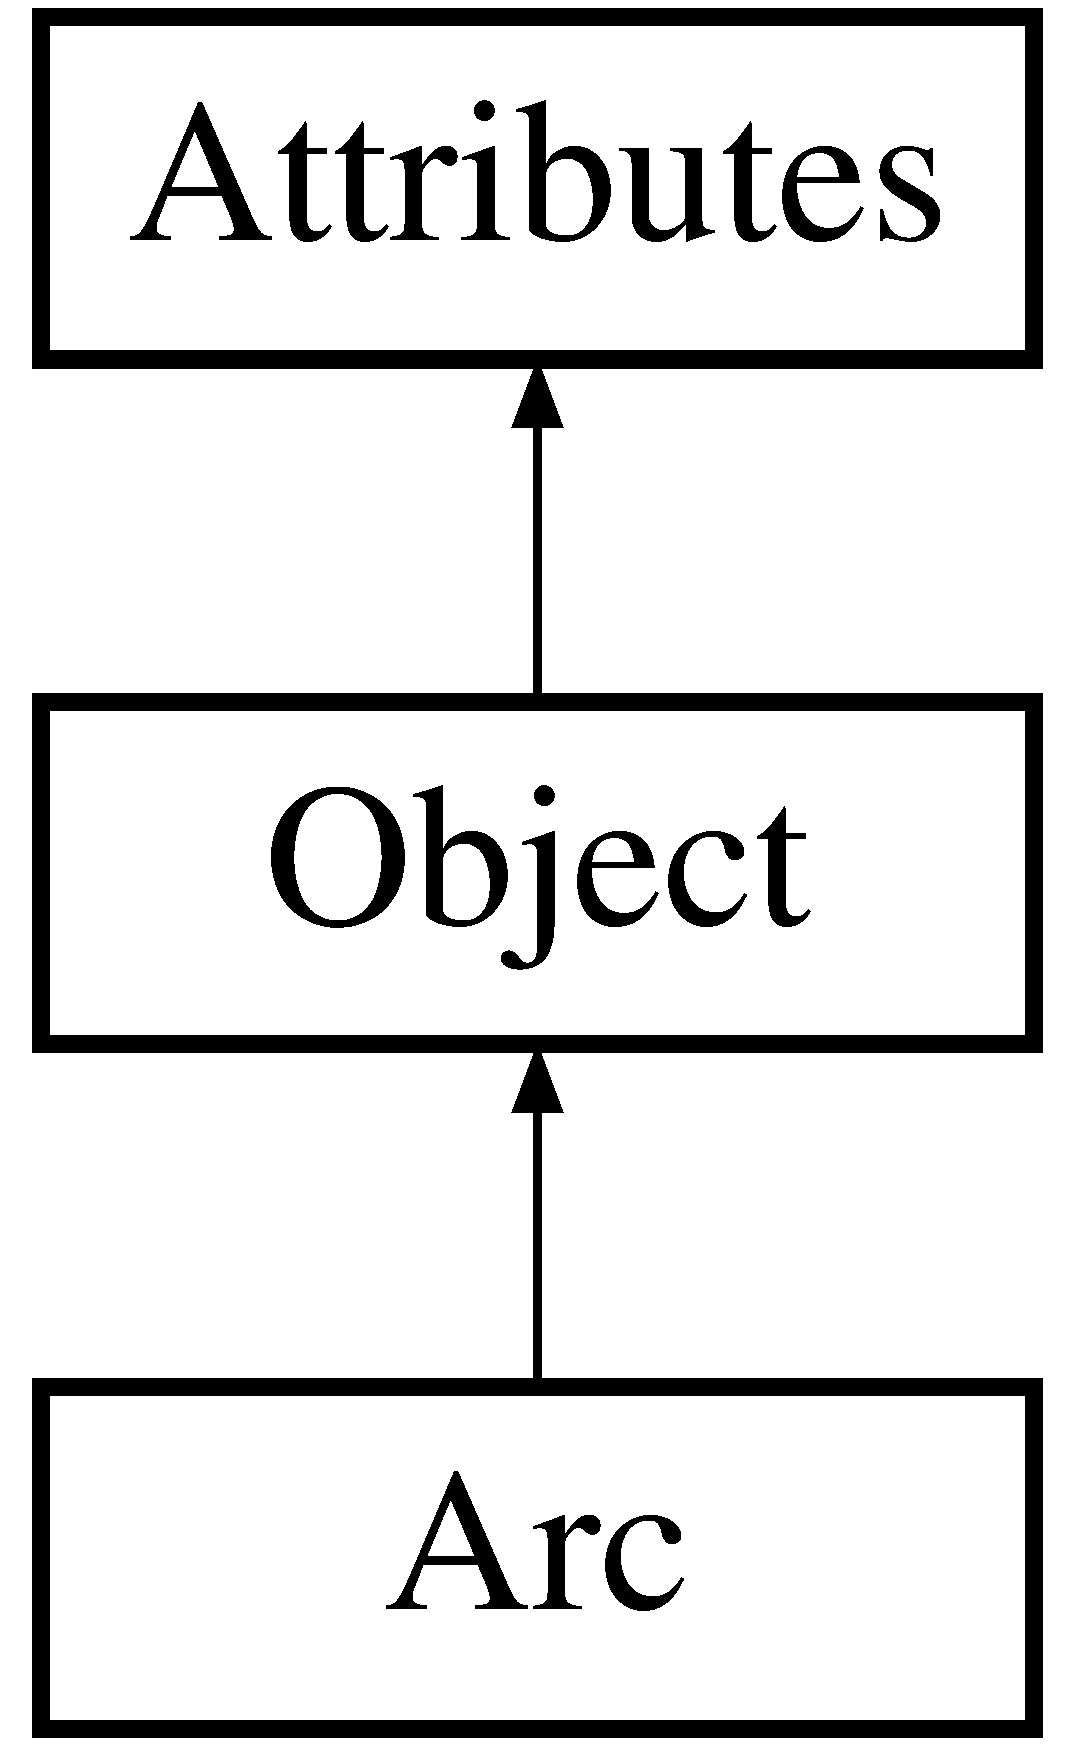
\includegraphics[height=3cm]{classArc}
\end{center}
\end{figure}
\subsection*{Public Types}
\begin{CompactItemize}
\item 
enum {\bf Directions} \{ {\bf Clockwise}, 
{\bf Counter\-Clockwise}
 \}
\item 
enum {\bf Arc\-Types} \{ {\bf Pie\-Wedged} =  0, 
{\bf Open\-Ended} =  1
 \}
\end{CompactItemize}
\subsection*{Public Methods}
\begin{CompactItemize}
\item 
{\bf Arc} ()
\item 
{\bf Arc} ({\bf Coordinate} $\ast$point1, {\bf Coordinate} $\ast$point2, {\bf Coordinate} $\ast$point3)
\item 
{\bf $\sim$Arc} ()
\item 
void {\bf set\-Arc\-Type} ({\bf Arc\-Types} {\bf arc\-Type})
\item 
{\bf Arc\-Types} {\bf get\-Arc\-Type} ()
\item 
{\bf Directions} {\bf get\-Direction} ()
\item 
void {\bf write} (std::ostream \&stream) const
\end{CompactItemize}
\subsection*{Protected Methods}
\begin{CompactItemize}
\item 
void {\bf set\-Direction} ({\bf Directions} {\bf direction})
\item 
double {\bf circum\-Center\-X} ()
\item 
double {\bf circum\-Center\-Y} ()
\item 
{\bf Directions} {\bf clockwise} ()
\item 
double {\bf determinant} (double a1, double a2, double a3, double b1, double b2, double b3, double c1, double c2, double c3)
\end{CompactItemize}
\subsection*{Protected Attributes}
\begin{CompactItemize}
\item 
{\bf Arc\-Types} {\bf arc\-Type}
\item 
{\bf Directions} {\bf direction}
\item 
double {\bf center\-X}
\item 
double {\bf center\-Y}
\item 
{\bf Coordinate} $\ast$ {\bf p1}
\item 
{\bf Coordinate} $\ast$ {\bf p2}
\item 
{\bf Coordinate} $\ast$ {\bf p3}
\end{CompactItemize}


\subsection{Detailed Description}
This class handles arc objects. This class is derived from {\bf Object} {\rm (p.\,\pageref{classObject})}. \begin{Desc}
\item[Author: ]\par
Anthony Liekens \end{Desc}




\subsection{Member Enumeration Documentation}
\index{Arc@{Arc}!ArcTypes@{ArcTypes}}
\index{ArcTypes@{ArcTypes}!Arc@{Arc}}
\subsubsection{\setlength{\rightskip}{0pt plus 5cm}enum Arc::Arc\-Types}\label{classArc_s5}


Enumeration of arc types. The following types can be used to set the type of an arc object : \{$\backslash$tt Pie\-Wedged, Open\-Ended\} \begin{Desc}
\item[Enumeration values: ]\par
\begin{description}
\index{PieWedged@{PieWedged}!Arc@{Arc}}\index{Arc@{Arc}!PieWedged@{PieWedged}}\item[{\em 
{\em Pie\-Wedged}\label{classArc_s5s2}
}]\index{OpenEnded@{OpenEnded}!Arc@{Arc}}\index{Arc@{Arc}!OpenEnded@{OpenEnded}}\item[{\em 
{\em Open\-Ended}\label{classArc_s5s3}
}]\end{description}
\end{Desc}

\index{Arc@{Arc}!Directions@{Directions}}
\index{Directions@{Directions}!Arc@{Arc}}
\subsubsection{\setlength{\rightskip}{0pt plus 5cm}enum Arc::Directions}\label{classArc_s4}


Enumeration of arc directions. The following directions can be used to set the direction of an arc object : \{$\backslash$tt Clockwise, Counter\-Clockwise\} \begin{Desc}
\item[Enumeration values: ]\par
\begin{description}
\index{Clockwise@{Clockwise}!Arc@{Arc}}\index{Arc@{Arc}!Clockwise@{Clockwise}}\item[{\em 
{\em Clockwise}\label{classArc_s4s0}
}]\index{CounterClockwise@{CounterClockwise}!Arc@{Arc}}\index{Arc@{Arc}!CounterClockwise@{CounterClockwise}}\item[{\em 
{\em Counter\-Clockwise}\label{classArc_s4s1}
}]\end{description}
\end{Desc}



\subsection{Constructor \& Destructor Documentation}
\index{Arc@{Arc}!Arc@{Arc}}
\index{Arc@{Arc}!Arc@{Arc}}
\subsubsection{\setlength{\rightskip}{0pt plus 5cm}Arc::Arc ()}\label{classArc_a0}


Constructor. Constructs an arc object. \index{Arc@{Arc}!Arc@{Arc}}
\index{Arc@{Arc}!Arc@{Arc}}
\subsubsection{\setlength{\rightskip}{0pt plus 5cm}Arc::Arc ({\bf Coordinate} $\ast$ {\em point1}, {\bf Coordinate} $\ast$ {\em point2}, {\bf Coordinate} $\ast$ {\em point3})}\label{classArc_a1}


Constructor. Constructs an arc object. An arc is defined by giving three points, a start point, an intermediate point and an end point. These three points lay on the arc. \begin{Desc}
\item[Parameters: ]\par
\begin{description}
\item[{\em 
point1}]First {\bf Coordinate} {\rm (p.\,\pageref{classCoordinate})} defining the arc \item[{\em 
point2}]Second {\bf Coordinate} {\rm (p.\,\pageref{classCoordinate})} defining the arc \item[{\em 
point3}]Third {\bf Coordinate} {\rm (p.\,\pageref{classCoordinate})} defining the arc \end{description}
\end{Desc}
\index{Arc@{Arc}!~Arc@{$\sim$Arc}}
\index{~Arc@{$\sim$Arc}!Arc@{Arc}}
\subsubsection{\setlength{\rightskip}{0pt plus 5cm}Arc::$\sim$Arc ()}\label{classArc_a2}


Destructor. Destructs an arc object. 

\subsection{Member Function Documentation}
\index{Arc@{Arc}!circumCenterX@{circumCenterX}}
\index{circumCenterX@{circumCenterX}!Arc@{Arc}}
\subsubsection{\setlength{\rightskip}{0pt plus 5cm}double Arc::circum\-Center\-X ()\hspace{0.3cm}{\tt  [protected]}}\label{classArc_b1}


Returns the x coordinate of the center of the arc object. \begin{Desc}
\item[Returns: ]\par
double \end{Desc}
\index{Arc@{Arc}!circumCenterY@{circumCenterY}}
\index{circumCenterY@{circumCenterY}!Arc@{Arc}}
\subsubsection{\setlength{\rightskip}{0pt plus 5cm}double Arc::circum\-Center\-Y ()\hspace{0.3cm}{\tt  [protected]}}\label{classArc_b2}


Returns the y coordinate of the center of the arc object. \begin{Desc}
\item[Returns: ]\par
double \end{Desc}
\index{Arc@{Arc}!clockwise@{clockwise}}
\index{clockwise@{clockwise}!Arc@{Arc}}
\subsubsection{\setlength{\rightskip}{0pt plus 5cm}{\bf Arc::Directions} Arc::clockwise ()\hspace{0.3cm}{\tt  [protected]}}\label{classArc_b3}


Calculates the direction of the arc object. \begin{Desc}
\item[Returns: ]\par
{\bf Directions} {\rm (p.\,\pageref{classArc_s4})} \end{Desc}
\index{Arc@{Arc}!determinant@{determinant}}
\index{determinant@{determinant}!Arc@{Arc}}
\subsubsection{\setlength{\rightskip}{0pt plus 5cm}double Arc::determinant (double {\em a1}, double {\em a2}, double {\em a3}, double {\em b1}, double {\em b2}, double {\em b3}, double {\em c1}, double {\em c2}, double {\em c3})\hspace{0.3cm}{\tt  [protected]}}\label{classArc_b4}


Returns the determinant of a 3 by 3 matrix. this function is needed for calculating the circumcenter of an arc, and the direction. \begin{Desc}
\item[Parameters: ]\par
\begin{description}
\item[{\em 
a1}]element on row 1, column 1 \item[{\em 
a2}]element on row 1, column 2 \item[{\em 
a3}]element on row 1, column 3 \item[{\em 
b1}]element on row 2, column 1 \item[{\em 
b2}]element on row 2, column 2 \item[{\em 
b3}]element on row 2, column 3 \item[{\em 
c1}]element on row 3, column 1 \item[{\em 
c2}]element on row 3, column 2 \item[{\em 
c3}]element on row 3, column 3 \end{description}
\end{Desc}
\begin{Desc}
\item[Returns: ]\par
double \end{Desc}
\index{Arc@{Arc}!getArcType@{getArcType}}
\index{getArcType@{getArcType}!Arc@{Arc}}
\subsubsection{\setlength{\rightskip}{0pt plus 5cm}{\bf Arc\-Types} Arc::get\-Arc\-Type ()\hspace{0.3cm}{\tt  [inline]}}\label{classArc_a4}


Returns the type of the arc object. \begin{Desc}
\item[Returns: ]\par
{\bf Arc\-Types} {\rm (p.\,\pageref{classArc_s5})} \end{Desc}
\index{Arc@{Arc}!getDirection@{getDirection}}
\index{getDirection@{getDirection}!Arc@{Arc}}
\subsubsection{\setlength{\rightskip}{0pt plus 5cm}{\bf Directions} Arc::get\-Direction ()\hspace{0.3cm}{\tt  [inline]}}\label{classArc_a5}


Returns the direction of the arc object. \begin{Desc}
\item[Returns: ]\par
{\bf Directions} {\rm (p.\,\pageref{classArc_s4})} \end{Desc}
\index{Arc@{Arc}!setArcType@{setArcType}}
\index{setArcType@{setArcType}!Arc@{Arc}}
\subsubsection{\setlength{\rightskip}{0pt plus 5cm}void Arc::set\-Arc\-Type ({\bf Arc\-Types} {\em arc\-Type})\hspace{0.3cm}{\tt  [inline]}}\label{classArc_a3}


Set the arc type \begin{Desc}
\item[Parameters: ]\par
\begin{description}
\item[{\em 
arc\-Type}]{\bf Arc\-Types} {\rm (p.\,\pageref{classArc_s5})} \end{description}
\end{Desc}
\begin{Desc}
\item[Returns: ]\par
void \end{Desc}
\index{Arc@{Arc}!setDirection@{setDirection}}
\index{setDirection@{setDirection}!Arc@{Arc}}
\subsubsection{\setlength{\rightskip}{0pt plus 5cm}void Arc::set\-Direction ({\bf Directions} {\em direction})\hspace{0.3cm}{\tt  [inline, protected]}}\label{classArc_b0}


Set the arc direction \begin{Desc}
\item[Parameters: ]\par
\begin{description}
\item[{\em 
direction}]{\bf Directions} {\rm (p.\,\pageref{classArc_s4})} \end{description}
\end{Desc}
\begin{Desc}
\item[Returns: ]\par
void \end{Desc}
\index{Arc@{Arc}!write@{write}}
\index{write@{write}!Arc@{Arc}}
\subsubsection{\setlength{\rightskip}{0pt plus 5cm}void Arc::write (std::ostream \& {\em stream}) const\hspace{0.3cm}{\tt  [virtual]}}\label{classArc_a6}


Write the arc object to a given outstream. \begin{Desc}
\item[Parameters: ]\par
\begin{description}
\item[{\em 
stream}]output stream \end{description}
\end{Desc}
\begin{Desc}
\item[Returns: ]\par
void \end{Desc}


Reimplemented from {\bf Object} {\rm (p.\,\pageref{classObject_a3})}.

\subsection{Member Data Documentation}
\index{Arc@{Arc}!arcType@{arcType}}
\index{arcType@{arcType}!Arc@{Arc}}
\subsubsection{\setlength{\rightskip}{0pt plus 5cm}{\bf Arc\-Types} Arc::arc\-Type\hspace{0.3cm}{\tt  [protected]}}\label{classArc_n0}


\index{Arc@{Arc}!centerX@{centerX}}
\index{centerX@{centerX}!Arc@{Arc}}
\subsubsection{\setlength{\rightskip}{0pt plus 5cm}double Arc::center\-X\hspace{0.3cm}{\tt  [protected]}}\label{classArc_n2}


\index{Arc@{Arc}!centerY@{centerY}}
\index{centerY@{centerY}!Arc@{Arc}}
\subsubsection{\setlength{\rightskip}{0pt plus 5cm}double Arc::center\-Y\hspace{0.3cm}{\tt  [protected]}}\label{classArc_n3}


\index{Arc@{Arc}!direction@{direction}}
\index{direction@{direction}!Arc@{Arc}}
\subsubsection{\setlength{\rightskip}{0pt plus 5cm}{\bf Directions} Arc::direction\hspace{0.3cm}{\tt  [protected]}}\label{classArc_n1}


\index{Arc@{Arc}!p1@{p1}}
\index{p1@{p1}!Arc@{Arc}}
\subsubsection{\setlength{\rightskip}{0pt plus 5cm}{\bf Coordinate}$\ast$ Arc::p1\hspace{0.3cm}{\tt  [protected]}}\label{classArc_n4}


\index{Arc@{Arc}!p2@{p2}}
\index{p2@{p2}!Arc@{Arc}}
\subsubsection{\setlength{\rightskip}{0pt plus 5cm}{\bf Coordinate} $\ast$ Arc::p2\hspace{0.3cm}{\tt  [protected]}}\label{classArc_n5}


\index{Arc@{Arc}!p3@{p3}}
\index{p3@{p3}!Arc@{Arc}}
\subsubsection{\setlength{\rightskip}{0pt plus 5cm}{\bf Coordinate} $\ast$ Arc::p3\hspace{0.3cm}{\tt  [protected]}}\label{classArc_n6}




The documentation for this class was generated from the following files:\begin{CompactItemize}
\item 
{\bf arc.h}\item 
{\bf arc.cpp}\end{CompactItemize}

\section{Arrow Class Reference}
\label{classArrow}\index{Arrow@{Arrow}}
{\tt \#include $<$arrow.h$>$}

\subsection*{Public Types}
\begin{CompactItemize}
\item 
enum {\bf Arrow\-Type} \{ {\bf Stick\-Arrow} =  0, 
{\bf Closed\-Triangle} =  1, 
{\bf Closed\-Intended} =  2, 
{\bf Closed\-Pointed} =  3
 \}
\item 
enum {\bf Arrow\-Style} \{ {\bf Hollow} =  0, 
{\bf Filled} =  1
 \}
\end{CompactItemize}
\subsection*{Public Methods}
\begin{CompactItemize}
\item 
{\bf Arrow} ()
\item 
{\bf $\sim$Arrow} ()
\item 
void {\bf set\-Type} ({\bf Arrow\-Type} {\bf type})
\item 
void {\bf set\-Style} ({\bf Arrow\-Style} {\bf style})
\item 
void {\bf set\-Thickness} (float {\bf thickness})
\item 
void {\bf set\-Width} (float {\bf width})
\item 
void {\bf set\-Height} (float {\bf height})
\item 
{\bf Arrow\-Type} {\bf get\-Type} ()
\item 
{\bf Arrow\-Style} {\bf get\-Style} ()
\item 
float {\bf get\-Thickness} ()
\item 
float {\bf get\-Width} ()
\item 
float {\bf get\-Height} ()
\item 
void {\bf write} (std::ostream \&stream) const
\end{CompactItemize}
\subsection*{Protected Attributes}
\begin{CompactItemize}
\item 
{\bf Arrow\-Type} {\bf type}
\item 
{\bf Arrow\-Style} {\bf style}
\item 
float {\bf thickness}
\item 
float {\bf width}
\item 
float {\bf height}
\end{CompactItemize}


\subsection{Detailed Description}
This class handles arrows objects. These arrows can be used at the start and end of {\bf Poly\-Line} {\rm (p.\,\pageref{classPolyLine})}, {\bf Arc} {\rm (p.\,\pageref{classArc})} and {\bf Spline} {\rm (p.\,\pageref{classSpline})} instances. See the {\bf Attributes::set\-Backward\-Arrow\-Bool} {\rm (p.\,\pageref{classAttributes_a14})}, {\bf Attributes::set\-Backward\-Arrow\-Bool} {\rm (p.\,\pageref{classAttributes_a14})}, {\bf Attributes::get\-Backward\-Arrow\-Bool} {\rm (p.\,\pageref{classAttributes_a36})}, {\bf Attributes::get\-Backward\-Arrow\-Bool} {\rm (p.\,\pageref{classAttributes_a36})}, {\bf Attributes::set\-Backward\-Arrow} {\rm (p.\,\pageref{classAttributes_a16})}, {\bf Attributes::set\-Backward\-Arrow} {\rm (p.\,\pageref{classAttributes_a16})}, {\bf Attributes::get\-Backward\-Arrow} {\rm (p.\,\pageref{classAttributes_a38})} and {\bf Attributes::get\-Backward\-Arrow} {\rm (p.\,\pageref{classAttributes_a38})} methods for how to use Arrow instances. \begin{Desc}
\item[Author: ]\par
Anthony Liekens \end{Desc}




\subsection{Member Enumeration Documentation}
\index{Arrow@{Arrow}!ArrowStyle@{ArrowStyle}}
\index{ArrowStyle@{ArrowStyle}!Arrow@{Arrow}}
\subsubsection{\setlength{\rightskip}{0pt plus 5cm}enum Arrow::Arrow\-Style}\label{classArrow_s7}


Enumeration of arrow styles. The following arrow styles can be used to set the style of an arrow object : \{$\backslash$tt Hollow, Filled\} \begin{Desc}
\item[Enumeration values: ]\par
\begin{description}
\index{Hollow@{Hollow}!Arrow@{Arrow}}\index{Arrow@{Arrow}!Hollow@{Hollow}}\item[{\em 
{\em Hollow}\label{classArrow_s7s4}
}]\index{Filled@{Filled}!Arrow@{Arrow}}\index{Arrow@{Arrow}!Filled@{Filled}}\item[{\em 
{\em Filled}\label{classArrow_s7s5}
}]\end{description}
\end{Desc}

\index{Arrow@{Arrow}!ArrowType@{ArrowType}}
\index{ArrowType@{ArrowType}!Arrow@{Arrow}}
\subsubsection{\setlength{\rightskip}{0pt plus 5cm}enum Arrow::Arrow\-Type}\label{classArrow_s6}


Enumeration of arrow types. The following arrow types can be used to set the type of an arrow object : \{$\backslash$tt Stick\-Arrow, Closed\-Triangle, Closed\-Intended, Closed\-Pointed\} \begin{Desc}
\item[Enumeration values: ]\par
\begin{description}
\index{StickArrow@{StickArrow}!Arrow@{Arrow}}\index{Arrow@{Arrow}!StickArrow@{StickArrow}}\item[{\em 
{\em Stick\-Arrow}\label{classArrow_s6s0}
}]\index{ClosedTriangle@{ClosedTriangle}!Arrow@{Arrow}}\index{Arrow@{Arrow}!ClosedTriangle@{ClosedTriangle}}\item[{\em 
{\em Closed\-Triangle}\label{classArrow_s6s1}
}]\index{ClosedIntended@{ClosedIntended}!Arrow@{Arrow}}\index{Arrow@{Arrow}!ClosedIntended@{ClosedIntended}}\item[{\em 
{\em Closed\-Intended}\label{classArrow_s6s2}
}]\index{ClosedPointed@{ClosedPointed}!Arrow@{Arrow}}\index{Arrow@{Arrow}!ClosedPointed@{ClosedPointed}}\item[{\em 
{\em Closed\-Pointed}\label{classArrow_s6s3}
}]\end{description}
\end{Desc}



\subsection{Constructor \& Destructor Documentation}
\index{Arrow@{Arrow}!Arrow@{Arrow}}
\index{Arrow@{Arrow}!Arrow@{Arrow}}
\subsubsection{\setlength{\rightskip}{0pt plus 5cm}Arrow::Arrow ()}\label{classArrow_a0}


Constructor. Constructs an Arrow instance \index{Arrow@{Arrow}!~Arrow@{$\sim$Arrow}}
\index{~Arrow@{$\sim$Arrow}!Arrow@{Arrow}}
\subsubsection{\setlength{\rightskip}{0pt plus 5cm}Arrow::$\sim$Arrow ()}\label{classArrow_a1}


Destructor. Destructs an Arrow instance 

\subsection{Member Function Documentation}
\index{Arrow@{Arrow}!getHeight@{getHeight}}
\index{getHeight@{getHeight}!Arrow@{Arrow}}
\subsubsection{\setlength{\rightskip}{0pt plus 5cm}float Arrow::get\-Height ()\hspace{0.3cm}{\tt  [inline]}}\label{classArrow_a11}


Returns the height. \begin{Desc}
\item[Returns: ]\par
float \end{Desc}
\index{Arrow@{Arrow}!getStyle@{getStyle}}
\index{getStyle@{getStyle}!Arrow@{Arrow}}
\subsubsection{\setlength{\rightskip}{0pt plus 5cm}{\bf Arrow\-Style} Arrow::get\-Style ()\hspace{0.3cm}{\tt  [inline]}}\label{classArrow_a8}


Returns the style. \begin{Desc}
\item[Returns: ]\par
{\bf Arrow\-Style} {\rm (p.\,\pageref{classArrow_s7})} \end{Desc}
\index{Arrow@{Arrow}!getThickness@{getThickness}}
\index{getThickness@{getThickness}!Arrow@{Arrow}}
\subsubsection{\setlength{\rightskip}{0pt plus 5cm}float Arrow::get\-Thickness ()\hspace{0.3cm}{\tt  [inline]}}\label{classArrow_a9}


Returns the thickness. \begin{Desc}
\item[Returns: ]\par
float \end{Desc}
\index{Arrow@{Arrow}!getType@{getType}}
\index{getType@{getType}!Arrow@{Arrow}}
\subsubsection{\setlength{\rightskip}{0pt plus 5cm}{\bf Arrow\-Type} Arrow::get\-Type ()\hspace{0.3cm}{\tt  [inline]}}\label{classArrow_a7}


Returns the type. \begin{Desc}
\item[Returns: ]\par
{\bf Arrow\-Type} {\rm (p.\,\pageref{classArrow_s6})} \end{Desc}
\index{Arrow@{Arrow}!getWidth@{getWidth}}
\index{getWidth@{getWidth}!Arrow@{Arrow}}
\subsubsection{\setlength{\rightskip}{0pt plus 5cm}float Arrow::get\-Width ()\hspace{0.3cm}{\tt  [inline]}}\label{classArrow_a10}


Returns the width. \begin{Desc}
\item[Returns: ]\par
float \end{Desc}
\index{Arrow@{Arrow}!setHeight@{setHeight}}
\index{setHeight@{setHeight}!Arrow@{Arrow}}
\subsubsection{\setlength{\rightskip}{0pt plus 5cm}void Arrow::set\-Height (float {\em height})\hspace{0.3cm}{\tt  [inline]}}\label{classArrow_a6}


Set the height. \begin{Desc}
\item[Parameters: ]\par
\begin{description}
\item[{\em 
heigt}]float \end{description}
\end{Desc}
\begin{Desc}
\item[Returns: ]\par
void \end{Desc}
\index{Arrow@{Arrow}!setStyle@{setStyle}}
\index{setStyle@{setStyle}!Arrow@{Arrow}}
\subsubsection{\setlength{\rightskip}{0pt plus 5cm}void Arrow::set\-Style ({\bf Arrow\-Style} {\em style})\hspace{0.3cm}{\tt  [inline]}}\label{classArrow_a3}


Set the style. \begin{Desc}
\item[Parameters: ]\par
\begin{description}
\item[{\em 
style}]{\bf Arrow\-Style} {\rm (p.\,\pageref{classArrow_s7})} \end{description}
\end{Desc}
\begin{Desc}
\item[Returns: ]\par
void \end{Desc}
\index{Arrow@{Arrow}!setThickness@{setThickness}}
\index{setThickness@{setThickness}!Arrow@{Arrow}}
\subsubsection{\setlength{\rightskip}{0pt plus 5cm}void Arrow::set\-Thickness (float {\em thickness})\hspace{0.3cm}{\tt  [inline]}}\label{classArrow_a4}


Set the thickness. \begin{Desc}
\item[Parameters: ]\par
\begin{description}
\item[{\em 
thickness}]float \end{description}
\end{Desc}
\begin{Desc}
\item[Returns: ]\par
void \end{Desc}
\index{Arrow@{Arrow}!setType@{setType}}
\index{setType@{setType}!Arrow@{Arrow}}
\subsubsection{\setlength{\rightskip}{0pt plus 5cm}void Arrow::set\-Type ({\bf Arrow\-Type} {\em type})\hspace{0.3cm}{\tt  [inline]}}\label{classArrow_a2}


Set the type. \begin{Desc}
\item[Parameters: ]\par
\begin{description}
\item[{\em 
type}]{\bf Arrow\-Type} {\rm (p.\,\pageref{classArrow_s6})} \end{description}
\end{Desc}
\begin{Desc}
\item[Returns: ]\par
void \end{Desc}
\index{Arrow@{Arrow}!setWidth@{setWidth}}
\index{setWidth@{setWidth}!Arrow@{Arrow}}
\subsubsection{\setlength{\rightskip}{0pt plus 5cm}void Arrow::set\-Width (float {\em width})\hspace{0.3cm}{\tt  [inline]}}\label{classArrow_a5}


Set the width. \begin{Desc}
\item[Parameters: ]\par
\begin{description}
\item[{\em 
width}]float \end{description}
\end{Desc}
\begin{Desc}
\item[Returns: ]\par
void \end{Desc}
\index{Arrow@{Arrow}!write@{write}}
\index{write@{write}!Arrow@{Arrow}}
\subsubsection{\setlength{\rightskip}{0pt plus 5cm}void Arrow::write (std::ostream \& {\em stream}) const}\label{classArrow_a12}


Write the coordinate object to a given outstream. \begin{Desc}
\item[Parameters: ]\par
\begin{description}
\item[{\em 
stream}]output stream \end{description}
\end{Desc}
\begin{Desc}
\item[Returns: ]\par
void \end{Desc}


\subsection{Member Data Documentation}
\index{Arrow@{Arrow}!height@{height}}
\index{height@{height}!Arrow@{Arrow}}
\subsubsection{\setlength{\rightskip}{0pt plus 5cm}float Arrow::height\hspace{0.3cm}{\tt  [protected]}}\label{classArrow_n4}


\index{Arrow@{Arrow}!style@{style}}
\index{style@{style}!Arrow@{Arrow}}
\subsubsection{\setlength{\rightskip}{0pt plus 5cm}{\bf Arrow\-Style} Arrow::style\hspace{0.3cm}{\tt  [protected]}}\label{classArrow_n1}


\index{Arrow@{Arrow}!thickness@{thickness}}
\index{thickness@{thickness}!Arrow@{Arrow}}
\subsubsection{\setlength{\rightskip}{0pt plus 5cm}float Arrow::thickness\hspace{0.3cm}{\tt  [protected]}}\label{classArrow_n2}


\index{Arrow@{Arrow}!type@{type}}
\index{type@{type}!Arrow@{Arrow}}
\subsubsection{\setlength{\rightskip}{0pt plus 5cm}{\bf Arrow\-Type} Arrow::type\hspace{0.3cm}{\tt  [protected]}}\label{classArrow_n0}


\index{Arrow@{Arrow}!width@{width}}
\index{width@{width}!Arrow@{Arrow}}
\subsubsection{\setlength{\rightskip}{0pt plus 5cm}float Arrow::width\hspace{0.3cm}{\tt  [protected]}}\label{classArrow_n3}




The documentation for this class was generated from the following files:\begin{CompactItemize}
\item 
{\bf arrow.h}\item 
{\bf arrow.cpp}\end{CompactItemize}

\section{Attributes Class Reference}
\label{classAttributes}\index{Attributes@{Attributes}}
{\tt \#include $<$attributes.h$>$}

Inheritance diagram for Attributes::\begin{figure}[H]
\begin{center}
\leavevmode
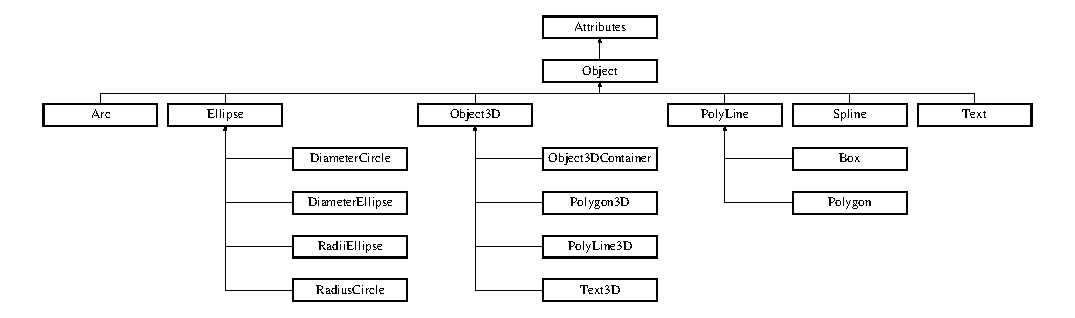
\includegraphics[height=3.82812cm]{classAttributes}
\end{center}
\end{figure}
\subsection*{Public Types}
\begin{CompactItemize}
\item 
enum {\bf Line\-Styles} \{ {\bf Default\-Line\-Style} =  -1, 
{\bf Solid} =  0, 
{\bf Dashed} =  1, 
{\bf Dotted} =  2, 
{\bf Dash\-Dotted} =  3, 
{\bf Dash\-Double\-Dotted} =  4, 
{\bf Dash\-Triple\-Dotted} =  5
 \}
\item 
enum {\bf Colors} \{ {\bf Default\-Color} =  -1, 
{\bf Black} =  0, 
{\bf Blue} =  1, 
{\bf Green} =  2, 
{\bf Cyan} =  3, 
{\bf Red} =  4, 
{\bf Magenta} =  5, 
{\bf Yellow} =  6, 
{\bf White} =  7, 
{\bf Gold} =  31
 \}
\item 
enum {\bf Fonts} \{ {\bf Default\-Latex} =  0, 
{\bf Roman} =  1, 
{\bf Bold} =  2, 
{\bf Italic} =  3, 
{\bf Sans\-Serif} =  4, 
{\bf Type\-Writer} =  5, 
{\bf Default\-Post\-Script} =  -1, 
{\bf Times\-Roman} =  0, 
{\bf Times\-Italic} =  1, 
{\bf Times\-Bold} =  2, 
{\bf Times\-Bold\-Italic} =  3, 
{\bf Avant\-Garde\-Book} =  4, 
{\bf Avant\-Garde\-Book\-Oblique} =  5, 
{\bf Avant\-Garde\-Demi} =  6, 
{\bf Avant\-Garde\-Demi\-Oblique} =  7, 
{\bf Bookman\-Light} =  8, 
{\bf Bookman\-Light\-Italic} =  9, 
{\bf Bookman\-Demi} =  10, 
{\bf Bookman\-Demi\-Italic} =  11, 
{\bf Courier} =  12, 
{\bf Courier\-Oblique} =  13, 
{\bf Courier\-Bold} =  14, 
{\bf Courier\-Bold\-Oblique} =  15, 
{\bf Helvetica} =  16, 
{\bf Helvetica\-Oblique} =  17, 
{\bf Helvetica\-Bold} =  18, 
{\bf Helvetica\-Bold\-Oblique} =  19, 
{\bf Helvetica\-Narrow} =  20, 
{\bf Helvetica\-Narrow\-Oblique} =  21, 
{\bf Helvetica\-Narrow\-Bold} =  22, 
{\bf Helvetica\-Narrow\-Bold\-Oblique} =  23, 
{\bf New\-Century\-Schoolbook\-Roman} =  24, 
{\bf New\-Century\-Schoolbook\-Italic} =  25, 
{\bf New\-Century\-Schoolbook\-Bold} =  26, 
{\bf New\-Century\-Schoolbook\-Bold\-Italic} =  27, 
{\bf Palatino\-Roman} =  28, 
{\bf Palatino\-Italic} =  29, 
{\bf Palatino\-Bold} =  30, 
{\bf Palatino\-Bold\-Italic} =  31, 
{\bf Symbol} =  32, 
{\bf Zapf\-Chancery\-Medium\-Italic} =  32, 
{\bf Zapf\-Dingbats} =  34
 \}
\item 
enum {\bf Font\-Flags} \{ {\bf Rigid} =  1, 
{\bf Latex} =  2, 
{\bf Rigid\-Latex} =  3, 
{\bf Post\-Script} =  4, 
{\bf Rigid\-Post\-Script} =  5, 
{\bf Latex\-Post\-Script} =  6, 
{\bf Rigid\-Latex\-Post\-Script} =  7, 
{\bf Hidden} =  8, 
{\bf Rigid\-Hidden} =  9, 
{\bf Latex\-Hidden} =  10, 
{\bf Rigid\-Latex\-Hidden} =  11, 
{\bf Post\-Script\-Hidden} =  12, 
{\bf Rigid\-Post\-Script\-Hidden} =  13, 
{\bf Latex\-Post\-Script\-Hidden} =  14, 
{\bf Rigid\-Latex\-Post\-Script\-Hidden} =  15
 \}
\end{CompactItemize}
\subsection*{Public Methods}
\begin{CompactItemize}
\item 
{\bf Attributes} ()
\item 
{\bf $\sim$Attributes} ()
\item 
void {\bf set\-Line\-Style} ({\bf Line\-Styles} {\bf line\-Style})
\item 
void {\bf set\-Thickness} (int {\bf thickness})
\item 
void {\bf set\-Pen\-Color} ({\bf Colors} {\bf pen\-Color})
\item 
void {\bf set\-Fill\-Color} ({\bf Colors} {\bf fill\-Color})
\item 
void {\bf set\-Depth} (int {\bf depth})
\item 
void {\bf set\-Pen\-Style} (int {\bf pen\-Style})
\item 
void {\bf set\-Area\-Fill} (int {\bf area\-Fill})
\item 
void {\bf set\-Style\-Val} (float {\bf style\-Val})
\item 
void {\bf set\-Join\-Style} (int {\bf join\-Style})
\item 
void {\bf set\-Cap\-Style} (int {\bf cap\-Style})
\item 
void {\bf set\-Radius} (int {\bf radius})
\item 
void {\bf set\-Forward\-Arrow\-Bool} (int {\bf forward\-Arrow\-Bool})
\item 
void {\bf set\-Backward\-Arrow\-Bool} (int {\bf backward\-Arrow\-Bool})
\item 
void {\bf set\-Forward\-Arrow} ({\bf Arrow} {\bf forward\-Arrow})
\item 
void {\bf set\-Backward\-Arrow} ({\bf Arrow} {\bf backward\-Arrow})
\item 
void {\bf set\-Angle} (float {\bf angle})
\item 
void {\bf set\-Font} ({\bf Fonts} {\bf font})
\item 
void {\bf set\-Font\-Size} (float {\bf font\-Size})
\item 
void {\bf set\-Font\-Flags} ({\bf Font\-Flags} {\bf font\-Flags})
\item 
void {\bf set\-Height} (float {\bf height})
\item 
void {\bf set\-Length} (float {\bf length})
\item 
void {\bf set\-Attributes} (Attributes attributes)
\item 
{\bf Line\-Styles} {\bf get\-Line\-Style} ()
\item 
int {\bf get\-Thickness} ()
\item 
{\bf Colors} {\bf get\-Pen\-Color} ()
\item 
{\bf Colors} {\bf get\-Fill\-Color} ()
\item 
int {\bf get\-Depth} ()
\item 
int {\bf get\-Pen\-Style} ()
\item 
int {\bf get\-Area\-Fill} ()
\item 
float {\bf get\-Style\-Val} ()
\item 
int {\bf get\-Join\-Style} ()
\item 
int {\bf get\-Cap\-Style} ()
\item 
int {\bf get\-Radius} ()
\item 
int {\bf get\-Forward\-Arrow\-Bool} ()
\item 
int {\bf get\-Backward\-Arrow\-Bool} ()
\item 
{\bf Arrow} {\bf get\-Forward\-Arrow} ()
\item 
{\bf Arrow} {\bf get\-Backward\-Arrow} ()
\item 
float {\bf get\-Angle} ()
\item 
{\bf Fonts} {\bf get\-Font} ()
\item 
float {\bf get\-Font\-Size} ()
\item 
{\bf Font\-Flags} {\bf get\-Font\-Flags} ()
\item 
float {\bf get\-Height} ()
\item 
float {\bf get\-Length} ()
\item 
Attributes {\bf get\-Attributes} ()
\end{CompactItemize}
\subsection*{Protected Attributes}
\begin{CompactItemize}
\item 
{\bf Line\-Styles} {\bf line\-Style}
\item 
int {\bf thickness}
\item 
{\bf Colors} {\bf pen\-Color}
\item 
{\bf Colors} {\bf fill\-Color}
\item 
int {\bf depth}
\item 
int {\bf pen\-Style}
\item 
int {\bf area\-Fill}
\item 
float {\bf style\-Val}
\item 
int {\bf join\-Style}
\item 
int {\bf cap\-Style}
\item 
int {\bf radius}
\item 
int {\bf forward\-Arrow\-Bool}
\item 
int {\bf backward\-Arrow\-Bool}
\item 
float {\bf angle}
\item 
{\bf Fonts} {\bf font}
\item 
float {\bf font\-Size}
\item 
{\bf Font\-Flags} {\bf font\-Flags}
\item 
float {\bf height}
\item 
float {\bf length}
\item 
{\bf Arrow} {\bf forward\-Arrow}
\item 
{\bf Arrow} {\bf backward\-Arrow}
\end{CompactItemize}


\subsection{Detailed Description}
Generic class to handle the attributes of objects. \begin{Desc}
\item[Author: ]\par
Anthony Liekens \end{Desc}




\subsection{Member Enumeration Documentation}
\index{Attributes@{Attributes}!Colors@{Colors}}
\index{Colors@{Colors}!Attributes@{Attributes}}
\subsubsection{\setlength{\rightskip}{0pt plus 5cm}enum Attributes::Colors}\label{classAttributes_s75}


\begin{Desc}
\item[Enumeration values: ]\par
\begin{description}
\index{DefaultColor@{DefaultColor}!Attributes@{Attributes}}\index{Attributes@{Attributes}!DefaultColor@{DefaultColor}}\item[{\em 
{\em Default\-Color}\label{classAttributes_s75s7}
}]\index{Black@{Black}!Attributes@{Attributes}}\index{Attributes@{Attributes}!Black@{Black}}\item[{\em 
{\em Black}\label{classAttributes_s75s8}
}]\index{Blue@{Blue}!Attributes@{Attributes}}\index{Attributes@{Attributes}!Blue@{Blue}}\item[{\em 
{\em Blue}\label{classAttributes_s75s9}
}]\index{Green@{Green}!Attributes@{Attributes}}\index{Attributes@{Attributes}!Green@{Green}}\item[{\em 
{\em Green}\label{classAttributes_s75s10}
}]\index{Cyan@{Cyan}!Attributes@{Attributes}}\index{Attributes@{Attributes}!Cyan@{Cyan}}\item[{\em 
{\em Cyan}\label{classAttributes_s75s11}
}]\index{Red@{Red}!Attributes@{Attributes}}\index{Attributes@{Attributes}!Red@{Red}}\item[{\em 
{\em Red}\label{classAttributes_s75s12}
}]\index{Magenta@{Magenta}!Attributes@{Attributes}}\index{Attributes@{Attributes}!Magenta@{Magenta}}\item[{\em 
{\em Magenta}\label{classAttributes_s75s13}
}]\index{Yellow@{Yellow}!Attributes@{Attributes}}\index{Attributes@{Attributes}!Yellow@{Yellow}}\item[{\em 
{\em Yellow}\label{classAttributes_s75s14}
}]\index{White@{White}!Attributes@{Attributes}}\index{Attributes@{Attributes}!White@{White}}\item[{\em 
{\em White}\label{classAttributes_s75s15}
}]\index{Gold@{Gold}!Attributes@{Attributes}}\index{Attributes@{Attributes}!Gold@{Gold}}\item[{\em 
{\em Gold}\label{classAttributes_s75s16}
}]\end{description}
\end{Desc}

\index{Attributes@{Attributes}!FontFlags@{FontFlags}}
\index{FontFlags@{FontFlags}!Attributes@{Attributes}}
\subsubsection{\setlength{\rightskip}{0pt plus 5cm}enum Attributes::Font\-Flags}\label{classAttributes_s77}


\begin{Desc}
\item[Enumeration values: ]\par
\begin{description}
\index{Rigid@{Rigid}!Attributes@{Attributes}}\index{Attributes@{Attributes}!Rigid@{Rigid}}\item[{\em 
{\em Rigid}\label{classAttributes_s77s59}
}]\index{Latex@{Latex}!Attributes@{Attributes}}\index{Attributes@{Attributes}!Latex@{Latex}}\item[{\em 
{\em Latex}\label{classAttributes_s77s60}
}]\index{RigidLatex@{RigidLatex}!Attributes@{Attributes}}\index{Attributes@{Attributes}!RigidLatex@{RigidLatex}}\item[{\em 
{\em Rigid\-Latex}\label{classAttributes_s77s61}
}]\index{PostScript@{PostScript}!Attributes@{Attributes}}\index{Attributes@{Attributes}!PostScript@{PostScript}}\item[{\em 
{\em Post\-Script}\label{classAttributes_s77s62}
}]\index{RigidPostScript@{RigidPostScript}!Attributes@{Attributes}}\index{Attributes@{Attributes}!RigidPostScript@{RigidPostScript}}\item[{\em 
{\em Rigid\-Post\-Script}\label{classAttributes_s77s63}
}]\index{LatexPostScript@{LatexPostScript}!Attributes@{Attributes}}\index{Attributes@{Attributes}!LatexPostScript@{LatexPostScript}}\item[{\em 
{\em Latex\-Post\-Script}\label{classAttributes_s77s64}
}]\index{RigidLatexPostScript@{RigidLatexPostScript}!Attributes@{Attributes}}\index{Attributes@{Attributes}!RigidLatexPostScript@{RigidLatexPostScript}}\item[{\em 
{\em Rigid\-Latex\-Post\-Script}\label{classAttributes_s77s65}
}]\index{Hidden@{Hidden}!Attributes@{Attributes}}\index{Attributes@{Attributes}!Hidden@{Hidden}}\item[{\em 
{\em Hidden}\label{classAttributes_s77s66}
}]\index{RigidHidden@{RigidHidden}!Attributes@{Attributes}}\index{Attributes@{Attributes}!RigidHidden@{RigidHidden}}\item[{\em 
{\em Rigid\-Hidden}\label{classAttributes_s77s67}
}]\index{LatexHidden@{LatexHidden}!Attributes@{Attributes}}\index{Attributes@{Attributes}!LatexHidden@{LatexHidden}}\item[{\em 
{\em Latex\-Hidden}\label{classAttributes_s77s68}
}]\index{RigidLatexHidden@{RigidLatexHidden}!Attributes@{Attributes}}\index{Attributes@{Attributes}!RigidLatexHidden@{RigidLatexHidden}}\item[{\em 
{\em Rigid\-Latex\-Hidden}\label{classAttributes_s77s69}
}]\index{PostScriptHidden@{PostScriptHidden}!Attributes@{Attributes}}\index{Attributes@{Attributes}!PostScriptHidden@{PostScriptHidden}}\item[{\em 
{\em Post\-Script\-Hidden}\label{classAttributes_s77s70}
}]\index{RigidPostScriptHidden@{RigidPostScriptHidden}!Attributes@{Attributes}}\index{Attributes@{Attributes}!RigidPostScriptHidden@{RigidPostScriptHidden}}\item[{\em 
{\em Rigid\-Post\-Script\-Hidden}\label{classAttributes_s77s71}
}]\index{LatexPostScriptHidden@{LatexPostScriptHidden}!Attributes@{Attributes}}\index{Attributes@{Attributes}!LatexPostScriptHidden@{LatexPostScriptHidden}}\item[{\em 
{\em Latex\-Post\-Script\-Hidden}\label{classAttributes_s77s72}
}]\index{RigidLatexPostScriptHidden@{RigidLatexPostScriptHidden}!Attributes@{Attributes}}\index{Attributes@{Attributes}!RigidLatexPostScriptHidden@{RigidLatexPostScriptHidden}}\item[{\em 
{\em Rigid\-Latex\-Post\-Script\-Hidden}\label{classAttributes_s77s73}
}]\end{description}
\end{Desc}

\index{Attributes@{Attributes}!Fonts@{Fonts}}
\index{Fonts@{Fonts}!Attributes@{Attributes}}
\subsubsection{\setlength{\rightskip}{0pt plus 5cm}enum Attributes::Fonts}\label{classAttributes_s76}


Enumeration of font faces. The following fonts can be used to set the font face of an object : \{$\backslash$tt Default\-Latex, Roman, Bold, Italic, Sans\-Serif, Type\-Writer, Default\-Post\-Script, Times\-Roman, Times\-Italic, Times\-Bold, Times\-Bold\-Italic, Avant\-Garde\-Book, Avant\-Garde\-Book\-Oblique, Avant\-Garde\-Demi, Avant\-Garde\-Demi\-Oblique, Bookman\-Light, Bookman\-Light\-Italic, Bookman\-Demi, Bookman\-Demi\-Italic, Courier, Courier\-Oblique, Courier\-Bold, Courier\-Bold\-Oblique, Helvetica, Helvetica\-Oblique, Helvetica\-Bold, Helvetica\-Bold\-Oblique, Helvetica\-Narrow, Helvetica\-Narrow\-Oblique, Helvetica\-Narrow\-Bold, Helvetica\-Narrow\-Bold\-Oblique, New\-Century\-Schoolbook\-Roman, New\-Century\-Schoolbook\-Italic, New\-Century\-Schoolbook\-Bold, New\-Century\-Schoolbook\-Bold\-Italic, Palatino\-Roman, Palatino\-Italic, Palatino\-Bold, Palatino\-Bold\-Italic, Symbol, Zapf\-Chancery\-Medium\-Italic, Zapf\-Dingbats\} \begin{Desc}
\item[Enumeration values: ]\par
\begin{description}
\index{DefaultLatex@{DefaultLatex}!Attributes@{Attributes}}\index{Attributes@{Attributes}!DefaultLatex@{DefaultLatex}}\item[{\em 
{\em Default\-Latex}\label{classAttributes_s76s17}
}]\index{Roman@{Roman}!Attributes@{Attributes}}\index{Attributes@{Attributes}!Roman@{Roman}}\item[{\em 
{\em Roman}\label{classAttributes_s76s18}
}]\index{Bold@{Bold}!Attributes@{Attributes}}\index{Attributes@{Attributes}!Bold@{Bold}}\item[{\em 
{\em Bold}\label{classAttributes_s76s19}
}]\index{Italic@{Italic}!Attributes@{Attributes}}\index{Attributes@{Attributes}!Italic@{Italic}}\item[{\em 
{\em Italic}\label{classAttributes_s76s20}
}]\index{SansSerif@{SansSerif}!Attributes@{Attributes}}\index{Attributes@{Attributes}!SansSerif@{SansSerif}}\item[{\em 
{\em Sans\-Serif}\label{classAttributes_s76s21}
}]\index{TypeWriter@{TypeWriter}!Attributes@{Attributes}}\index{Attributes@{Attributes}!TypeWriter@{TypeWriter}}\item[{\em 
{\em Type\-Writer}\label{classAttributes_s76s22}
}]\index{DefaultPostScript@{DefaultPostScript}!Attributes@{Attributes}}\index{Attributes@{Attributes}!DefaultPostScript@{DefaultPostScript}}\item[{\em 
{\em Default\-Post\-Script}\label{classAttributes_s76s23}
}]\index{TimesRoman@{TimesRoman}!Attributes@{Attributes}}\index{Attributes@{Attributes}!TimesRoman@{TimesRoman}}\item[{\em 
{\em Times\-Roman}\label{classAttributes_s76s24}
}]\index{TimesItalic@{TimesItalic}!Attributes@{Attributes}}\index{Attributes@{Attributes}!TimesItalic@{TimesItalic}}\item[{\em 
{\em Times\-Italic}\label{classAttributes_s76s25}
}]\index{TimesBold@{TimesBold}!Attributes@{Attributes}}\index{Attributes@{Attributes}!TimesBold@{TimesBold}}\item[{\em 
{\em Times\-Bold}\label{classAttributes_s76s26}
}]\index{TimesBoldItalic@{TimesBoldItalic}!Attributes@{Attributes}}\index{Attributes@{Attributes}!TimesBoldItalic@{TimesBoldItalic}}\item[{\em 
{\em Times\-Bold\-Italic}\label{classAttributes_s76s27}
}]\index{AvantGardeBook@{AvantGardeBook}!Attributes@{Attributes}}\index{Attributes@{Attributes}!AvantGardeBook@{AvantGardeBook}}\item[{\em 
{\em Avant\-Garde\-Book}\label{classAttributes_s76s28}
}]\index{AvantGardeBookOblique@{AvantGardeBookOblique}!Attributes@{Attributes}}\index{Attributes@{Attributes}!AvantGardeBookOblique@{AvantGardeBookOblique}}\item[{\em 
{\em Avant\-Garde\-Book\-Oblique}\label{classAttributes_s76s29}
}]\index{AvantGardeDemi@{AvantGardeDemi}!Attributes@{Attributes}}\index{Attributes@{Attributes}!AvantGardeDemi@{AvantGardeDemi}}\item[{\em 
{\em Avant\-Garde\-Demi}\label{classAttributes_s76s30}
}]\index{AvantGardeDemiOblique@{AvantGardeDemiOblique}!Attributes@{Attributes}}\index{Attributes@{Attributes}!AvantGardeDemiOblique@{AvantGardeDemiOblique}}\item[{\em 
{\em Avant\-Garde\-Demi\-Oblique}\label{classAttributes_s76s31}
}]\index{BookmanLight@{BookmanLight}!Attributes@{Attributes}}\index{Attributes@{Attributes}!BookmanLight@{BookmanLight}}\item[{\em 
{\em Bookman\-Light}\label{classAttributes_s76s32}
}]\index{BookmanLightItalic@{BookmanLightItalic}!Attributes@{Attributes}}\index{Attributes@{Attributes}!BookmanLightItalic@{BookmanLightItalic}}\item[{\em 
{\em Bookman\-Light\-Italic}\label{classAttributes_s76s33}
}]\index{BookmanDemi@{BookmanDemi}!Attributes@{Attributes}}\index{Attributes@{Attributes}!BookmanDemi@{BookmanDemi}}\item[{\em 
{\em Bookman\-Demi}\label{classAttributes_s76s34}
}]\index{BookmanDemiItalic@{BookmanDemiItalic}!Attributes@{Attributes}}\index{Attributes@{Attributes}!BookmanDemiItalic@{BookmanDemiItalic}}\item[{\em 
{\em Bookman\-Demi\-Italic}\label{classAttributes_s76s35}
}]\index{Courier@{Courier}!Attributes@{Attributes}}\index{Attributes@{Attributes}!Courier@{Courier}}\item[{\em 
{\em Courier}\label{classAttributes_s76s36}
}]\index{CourierOblique@{CourierOblique}!Attributes@{Attributes}}\index{Attributes@{Attributes}!CourierOblique@{CourierOblique}}\item[{\em 
{\em Courier\-Oblique}\label{classAttributes_s76s37}
}]\index{CourierBold@{CourierBold}!Attributes@{Attributes}}\index{Attributes@{Attributes}!CourierBold@{CourierBold}}\item[{\em 
{\em Courier\-Bold}\label{classAttributes_s76s38}
}]\index{CourierBoldOblique@{CourierBoldOblique}!Attributes@{Attributes}}\index{Attributes@{Attributes}!CourierBoldOblique@{CourierBoldOblique}}\item[{\em 
{\em Courier\-Bold\-Oblique}\label{classAttributes_s76s39}
}]\index{Helvetica@{Helvetica}!Attributes@{Attributes}}\index{Attributes@{Attributes}!Helvetica@{Helvetica}}\item[{\em 
{\em Helvetica}\label{classAttributes_s76s40}
}]\index{HelveticaOblique@{HelveticaOblique}!Attributes@{Attributes}}\index{Attributes@{Attributes}!HelveticaOblique@{HelveticaOblique}}\item[{\em 
{\em Helvetica\-Oblique}\label{classAttributes_s76s41}
}]\index{HelveticaBold@{HelveticaBold}!Attributes@{Attributes}}\index{Attributes@{Attributes}!HelveticaBold@{HelveticaBold}}\item[{\em 
{\em Helvetica\-Bold}\label{classAttributes_s76s42}
}]\index{HelveticaBoldOblique@{HelveticaBoldOblique}!Attributes@{Attributes}}\index{Attributes@{Attributes}!HelveticaBoldOblique@{HelveticaBoldOblique}}\item[{\em 
{\em Helvetica\-Bold\-Oblique}\label{classAttributes_s76s43}
}]\index{HelveticaNarrow@{HelveticaNarrow}!Attributes@{Attributes}}\index{Attributes@{Attributes}!HelveticaNarrow@{HelveticaNarrow}}\item[{\em 
{\em Helvetica\-Narrow}\label{classAttributes_s76s44}
}]\index{HelveticaNarrowOblique@{HelveticaNarrowOblique}!Attributes@{Attributes}}\index{Attributes@{Attributes}!HelveticaNarrowOblique@{HelveticaNarrowOblique}}\item[{\em 
{\em Helvetica\-Narrow\-Oblique}\label{classAttributes_s76s45}
}]\index{HelveticaNarrowBold@{HelveticaNarrowBold}!Attributes@{Attributes}}\index{Attributes@{Attributes}!HelveticaNarrowBold@{HelveticaNarrowBold}}\item[{\em 
{\em Helvetica\-Narrow\-Bold}\label{classAttributes_s76s46}
}]\index{HelveticaNarrowBoldOblique@{HelveticaNarrowBoldOblique}!Attributes@{Attributes}}\index{Attributes@{Attributes}!HelveticaNarrowBoldOblique@{HelveticaNarrowBoldOblique}}\item[{\em 
{\em Helvetica\-Narrow\-Bold\-Oblique}\label{classAttributes_s76s47}
}]\index{NewCenturySchoolbookRoman@{NewCenturySchoolbookRoman}!Attributes@{Attributes}}\index{Attributes@{Attributes}!NewCenturySchoolbookRoman@{NewCenturySchoolbookRoman}}\item[{\em 
{\em New\-Century\-Schoolbook\-Roman}\label{classAttributes_s76s48}
}]\index{NewCenturySchoolbookItalic@{NewCenturySchoolbookItalic}!Attributes@{Attributes}}\index{Attributes@{Attributes}!NewCenturySchoolbookItalic@{NewCenturySchoolbookItalic}}\item[{\em 
{\em New\-Century\-Schoolbook\-Italic}\label{classAttributes_s76s49}
}]\index{NewCenturySchoolbookBold@{NewCenturySchoolbookBold}!Attributes@{Attributes}}\index{Attributes@{Attributes}!NewCenturySchoolbookBold@{NewCenturySchoolbookBold}}\item[{\em 
{\em New\-Century\-Schoolbook\-Bold}\label{classAttributes_s76s50}
}]\index{NewCenturySchoolbookBoldItalic@{NewCenturySchoolbookBoldItalic}!Attributes@{Attributes}}\index{Attributes@{Attributes}!NewCenturySchoolbookBoldItalic@{NewCenturySchoolbookBoldItalic}}\item[{\em 
{\em New\-Century\-Schoolbook\-Bold\-Italic}\label{classAttributes_s76s51}
}]\index{PalatinoRoman@{PalatinoRoman}!Attributes@{Attributes}}\index{Attributes@{Attributes}!PalatinoRoman@{PalatinoRoman}}\item[{\em 
{\em Palatino\-Roman}\label{classAttributes_s76s52}
}]\index{PalatinoItalic@{PalatinoItalic}!Attributes@{Attributes}}\index{Attributes@{Attributes}!PalatinoItalic@{PalatinoItalic}}\item[{\em 
{\em Palatino\-Italic}\label{classAttributes_s76s53}
}]\index{PalatinoBold@{PalatinoBold}!Attributes@{Attributes}}\index{Attributes@{Attributes}!PalatinoBold@{PalatinoBold}}\item[{\em 
{\em Palatino\-Bold}\label{classAttributes_s76s54}
}]\index{PalatinoBoldItalic@{PalatinoBoldItalic}!Attributes@{Attributes}}\index{Attributes@{Attributes}!PalatinoBoldItalic@{PalatinoBoldItalic}}\item[{\em 
{\em Palatino\-Bold\-Italic}\label{classAttributes_s76s55}
}]\index{Symbol@{Symbol}!Attributes@{Attributes}}\index{Attributes@{Attributes}!Symbol@{Symbol}}\item[{\em 
{\em Symbol}\label{classAttributes_s76s56}
}]\index{ZapfChanceryMediumItalic@{ZapfChanceryMediumItalic}!Attributes@{Attributes}}\index{Attributes@{Attributes}!ZapfChanceryMediumItalic@{ZapfChanceryMediumItalic}}\item[{\em 
{\em Zapf\-Chancery\-Medium\-Italic}\label{classAttributes_s76s57}
}]\index{ZapfDingbats@{ZapfDingbats}!Attributes@{Attributes}}\index{Attributes@{Attributes}!ZapfDingbats@{ZapfDingbats}}\item[{\em 
{\em Zapf\-Dingbats}\label{classAttributes_s76s58}
}]\end{description}
\end{Desc}

\index{Attributes@{Attributes}!LineStyles@{LineStyles}}
\index{LineStyles@{LineStyles}!Attributes@{Attributes}}
\subsubsection{\setlength{\rightskip}{0pt plus 5cm}enum Attributes::Line\-Styles}\label{classAttributes_s74}


Enumeration of line styles. The following line styles can be used to set the line style of an object : \{$\backslash$tt Default\-Line\-Style, Solid, Dashed, Dotted, Dash\-Dotted, Dash\-Dotted, Dash\-Double\-Dotted, Dash\-Triple\-Dotted\} \begin{Desc}
\item[Enumeration values: ]\par
\begin{description}
\index{DefaultLineStyle@{DefaultLineStyle}!Attributes@{Attributes}}\index{Attributes@{Attributes}!DefaultLineStyle@{DefaultLineStyle}}\item[{\em 
{\em Default\-Line\-Style}\label{classAttributes_s74s0}
}]\index{Solid@{Solid}!Attributes@{Attributes}}\index{Attributes@{Attributes}!Solid@{Solid}}\item[{\em 
{\em Solid}\label{classAttributes_s74s1}
}]\index{Dashed@{Dashed}!Attributes@{Attributes}}\index{Attributes@{Attributes}!Dashed@{Dashed}}\item[{\em 
{\em Dashed}\label{classAttributes_s74s2}
}]\index{Dotted@{Dotted}!Attributes@{Attributes}}\index{Attributes@{Attributes}!Dotted@{Dotted}}\item[{\em 
{\em Dotted}\label{classAttributes_s74s3}
}]\index{DashDotted@{DashDotted}!Attributes@{Attributes}}\index{Attributes@{Attributes}!DashDotted@{DashDotted}}\item[{\em 
{\em Dash\-Dotted}\label{classAttributes_s74s4}
}]\index{DashDoubleDotted@{DashDoubleDotted}!Attributes@{Attributes}}\index{Attributes@{Attributes}!DashDoubleDotted@{DashDoubleDotted}}\item[{\em 
{\em Dash\-Double\-Dotted}\label{classAttributes_s74s5}
}]\index{DashTripleDotted@{DashTripleDotted}!Attributes@{Attributes}}\index{Attributes@{Attributes}!DashTripleDotted@{DashTripleDotted}}\item[{\em 
{\em Dash\-Triple\-Dotted}\label{classAttributes_s74s6}
}]\end{description}
\end{Desc}



\subsection{Constructor \& Destructor Documentation}
\index{Attributes@{Attributes}!Attributes@{Attributes}}
\index{Attributes@{Attributes}!Attributes@{Attributes}}
\subsubsection{\setlength{\rightskip}{0pt plus 5cm}Attributes::Attributes ()}\label{classAttributes_a0}


Constructor. Sets default values for all attributes. \index{Attributes@{Attributes}!~Attributes@{$\sim$Attributes}}
\index{~Attributes@{$\sim$Attributes}!Attributes@{Attributes}}
\subsubsection{\setlength{\rightskip}{0pt plus 5cm}Attributes::$\sim$Attributes ()}\label{classAttributes_a1}


Destructor. 

\subsection{Member Function Documentation}
\index{Attributes@{Attributes}!getAngle@{getAngle}}
\index{getAngle@{getAngle}!Attributes@{Attributes}}
\subsubsection{\setlength{\rightskip}{0pt plus 5cm}float Attributes::get\-Angle ()\hspace{0.3cm}{\tt  [inline]}}\label{classAttributes_a39}


Returns the angle. \begin{Desc}
\item[Returns: ]\par
float \end{Desc}


Reimplemented in {\bf Ellipse} {\rm (p.\,\pageref{classEllipse_a4})}.\index{Attributes@{Attributes}!getAreaFill@{getAreaFill}}
\index{getAreaFill@{getAreaFill}!Attributes@{Attributes}}
\subsubsection{\setlength{\rightskip}{0pt plus 5cm}int Attributes::get\-Area\-Fill ()\hspace{0.3cm}{\tt  [inline]}}\label{classAttributes_a30}


Returns the area fill. \begin{Desc}
\item[Returns: ]\par
int \end{Desc}
\index{Attributes@{Attributes}!getAttributes@{getAttributes}}
\index{getAttributes@{getAttributes}!Attributes@{Attributes}}
\subsubsection{\setlength{\rightskip}{0pt plus 5cm}Attributes Attributes::get\-Attributes ()\hspace{0.3cm}{\tt  [inline]}}\label{classAttributes_a45}


Returns itself. This method can be used to extract attributes out of {\bf Object} {\rm (p.\,\pageref{classObject})} instances. \begin{Desc}
\item[Returns: ]\par
Instance of Attributes \end{Desc}
\index{Attributes@{Attributes}!getBackwardArrow@{getBackwardArrow}}
\index{getBackwardArrow@{getBackwardArrow}!Attributes@{Attributes}}
\subsubsection{\setlength{\rightskip}{0pt plus 5cm}{\bf Arrow} Attributes::get\-Backward\-Arrow ()\hspace{0.3cm}{\tt  [inline]}}\label{classAttributes_a38}


Returns the backward arrow. \begin{Desc}
\item[Returns: ]\par
Instance of {\bf Arrow} {\rm (p.\,\pageref{classArrow})} \end{Desc}
\index{Attributes@{Attributes}!getBackwardArrowBool@{getBackwardArrowBool}}
\index{getBackwardArrowBool@{getBackwardArrowBool}!Attributes@{Attributes}}
\subsubsection{\setlength{\rightskip}{0pt plus 5cm}int Attributes::get\-Backward\-Arrow\-Bool ()\hspace{0.3cm}{\tt  [inline]}}\label{classAttributes_a36}


Returns the backward arrow bool value (0 = do not draw an arrow, 1 = draw an arrow). \begin{Desc}
\item[Returns: ]\par
int \end{Desc}
\index{Attributes@{Attributes}!getCapStyle@{getCapStyle}}
\index{getCapStyle@{getCapStyle}!Attributes@{Attributes}}
\subsubsection{\setlength{\rightskip}{0pt plus 5cm}int Attributes::get\-Cap\-Style ()\hspace{0.3cm}{\tt  [inline]}}\label{classAttributes_a33}


Returns the cap style. \begin{Desc}
\item[Returns: ]\par
int \end{Desc}
\index{Attributes@{Attributes}!getDepth@{getDepth}}
\index{getDepth@{getDepth}!Attributes@{Attributes}}
\subsubsection{\setlength{\rightskip}{0pt plus 5cm}int Attributes::get\-Depth ()\hspace{0.3cm}{\tt  [inline]}}\label{classAttributes_a28}


Returns the depth (layer depth). \begin{Desc}
\item[Returns: ]\par
int \end{Desc}
\index{Attributes@{Attributes}!getFillColor@{getFillColor}}
\index{getFillColor@{getFillColor}!Attributes@{Attributes}}
\subsubsection{\setlength{\rightskip}{0pt plus 5cm}{\bf Colors} Attributes::get\-Fill\-Color ()\hspace{0.3cm}{\tt  [inline]}}\label{classAttributes_a27}


Returns the fill color. \begin{Desc}
\item[Returns: ]\par
Instance of {\bf Attributes::Colors} {\rm (p.\,\pageref{classAttributes_s75})} \end{Desc}
\index{Attributes@{Attributes}!getFont@{getFont}}
\index{getFont@{getFont}!Attributes@{Attributes}}
\subsubsection{\setlength{\rightskip}{0pt plus 5cm}{\bf Fonts} Attributes::get\-Font ()\hspace{0.3cm}{\tt  [inline]}}\label{classAttributes_a40}


Returns the font face. \begin{Desc}
\item[Returns: ]\par
Instance of {\bf Attributes::Fonts} {\rm (p.\,\pageref{classAttributes_s76})} \end{Desc}
\index{Attributes@{Attributes}!getFontFlags@{getFontFlags}}
\index{getFontFlags@{getFontFlags}!Attributes@{Attributes}}
\subsubsection{\setlength{\rightskip}{0pt plus 5cm}{\bf Font\-Flags} Attributes::get\-Font\-Flags ()\hspace{0.3cm}{\tt  [inline]}}\label{classAttributes_a42}


Returns the font flags. \begin{Desc}
\item[Returns: ]\par
Instance of {\bf Attributes::Font\-Flags} {\rm (p.\,\pageref{classAttributes_s77})} \end{Desc}
\index{Attributes@{Attributes}!getFontSize@{getFontSize}}
\index{getFontSize@{getFontSize}!Attributes@{Attributes}}
\subsubsection{\setlength{\rightskip}{0pt plus 5cm}float Attributes::get\-Font\-Size ()\hspace{0.3cm}{\tt  [inline]}}\label{classAttributes_a41}


Returns the font size. \begin{Desc}
\item[Returns: ]\par
float \end{Desc}
\index{Attributes@{Attributes}!getForwardArrow@{getForwardArrow}}
\index{getForwardArrow@{getForwardArrow}!Attributes@{Attributes}}
\subsubsection{\setlength{\rightskip}{0pt plus 5cm}{\bf Arrow} Attributes::get\-Forward\-Arrow ()\hspace{0.3cm}{\tt  [inline]}}\label{classAttributes_a37}


Returns the forward arrow. \begin{Desc}
\item[Returns: ]\par
Instance of {\bf Arrow} {\rm (p.\,\pageref{classArrow})} \end{Desc}
\index{Attributes@{Attributes}!getForwardArrowBool@{getForwardArrowBool}}
\index{getForwardArrowBool@{getForwardArrowBool}!Attributes@{Attributes}}
\subsubsection{\setlength{\rightskip}{0pt plus 5cm}int Attributes::get\-Forward\-Arrow\-Bool ()\hspace{0.3cm}{\tt  [inline]}}\label{classAttributes_a35}


Returns the forward arrow bool value (0 = do not draw an arrow, 1 = draw an arrow). \begin{Desc}
\item[Returns: ]\par
int \end{Desc}
\index{Attributes@{Attributes}!getHeight@{getHeight}}
\index{getHeight@{getHeight}!Attributes@{Attributes}}
\subsubsection{\setlength{\rightskip}{0pt plus 5cm}float Attributes::get\-Height ()\hspace{0.3cm}{\tt  [inline]}}\label{classAttributes_a43}


Returns the font height (of bounding box). \begin{Desc}
\item[Returns: ]\par
float \end{Desc}
\index{Attributes@{Attributes}!getJoinStyle@{getJoinStyle}}
\index{getJoinStyle@{getJoinStyle}!Attributes@{Attributes}}
\subsubsection{\setlength{\rightskip}{0pt plus 5cm}int Attributes::get\-Join\-Style ()\hspace{0.3cm}{\tt  [inline]}}\label{classAttributes_a32}


Returns the join style. \begin{Desc}
\item[Returns: ]\par
int \end{Desc}
\index{Attributes@{Attributes}!getLength@{getLength}}
\index{getLength@{getLength}!Attributes@{Attributes}}
\subsubsection{\setlength{\rightskip}{0pt plus 5cm}float Attributes::get\-Length ()\hspace{0.3cm}{\tt  [inline]}}\label{classAttributes_a44}


Returns the font length (of bounding box). \begin{Desc}
\item[Returns: ]\par
float \end{Desc}
\index{Attributes@{Attributes}!getLineStyle@{getLineStyle}}
\index{getLineStyle@{getLineStyle}!Attributes@{Attributes}}
\subsubsection{\setlength{\rightskip}{0pt plus 5cm}{\bf Line\-Styles} Attributes::get\-Line\-Style ()\hspace{0.3cm}{\tt  [inline]}}\label{classAttributes_a24}


Returns the line style. \begin{Desc}
\item[Returns: ]\par
Instance of {\bf Attributes::Line\-Styles} {\rm (p.\,\pageref{classAttributes_s74})} \end{Desc}
\index{Attributes@{Attributes}!getPenColor@{getPenColor}}
\index{getPenColor@{getPenColor}!Attributes@{Attributes}}
\subsubsection{\setlength{\rightskip}{0pt plus 5cm}{\bf Colors} Attributes::get\-Pen\-Color ()\hspace{0.3cm}{\tt  [inline]}}\label{classAttributes_a26}


Returns the pen color. \begin{Desc}
\item[Returns: ]\par
Instance of {\bf Attributes::Colors} {\rm (p.\,\pageref{classAttributes_s75})} \end{Desc}
\index{Attributes@{Attributes}!getPenStyle@{getPenStyle}}
\index{getPenStyle@{getPenStyle}!Attributes@{Attributes}}
\subsubsection{\setlength{\rightskip}{0pt plus 5cm}int Attributes::get\-Pen\-Style ()\hspace{0.3cm}{\tt  [inline]}}\label{classAttributes_a29}


Returns the pen style. \begin{Desc}
\item[Returns: ]\par
int \end{Desc}
\index{Attributes@{Attributes}!getRadius@{getRadius}}
\index{getRadius@{getRadius}!Attributes@{Attributes}}
\subsubsection{\setlength{\rightskip}{0pt plus 5cm}int Attributes::get\-Radius ()\hspace{0.3cm}{\tt  [inline]}}\label{classAttributes_a34}


Returns the radius. \begin{Desc}
\item[Returns: ]\par
int \end{Desc}
\index{Attributes@{Attributes}!getStyleVal@{getStyleVal}}
\index{getStyleVal@{getStyleVal}!Attributes@{Attributes}}
\subsubsection{\setlength{\rightskip}{0pt plus 5cm}float Attributes::get\-Style\-Val ()\hspace{0.3cm}{\tt  [inline]}}\label{classAttributes_a31}


Returns the style value. \begin{Desc}
\item[Returns: ]\par
float \end{Desc}
\index{Attributes@{Attributes}!getThickness@{getThickness}}
\index{getThickness@{getThickness}!Attributes@{Attributes}}
\subsubsection{\setlength{\rightskip}{0pt plus 5cm}int Attributes::get\-Thickness ()\hspace{0.3cm}{\tt  [inline]}}\label{classAttributes_a25}


Returns the thickness. \begin{Desc}
\item[Returns: ]\par
int \end{Desc}
\index{Attributes@{Attributes}!setAngle@{setAngle}}
\index{setAngle@{setAngle}!Attributes@{Attributes}}
\subsubsection{\setlength{\rightskip}{0pt plus 5cm}void Attributes::set\-Angle (float {\em angle})\hspace{0.3cm}{\tt  [inline]}}\label{classAttributes_a17}


Set the angle. \begin{Desc}
\item[Parameters: ]\par
\begin{description}
\item[{\em 
angle}]float value \end{description}
\end{Desc}
\begin{Desc}
\item[Returns: ]\par
void \end{Desc}


Reimplemented in {\bf Ellipse} {\rm (p.\,\pageref{classEllipse_a3})}.\index{Attributes@{Attributes}!setAreaFill@{setAreaFill}}
\index{setAreaFill@{setAreaFill}!Attributes@{Attributes}}
\subsubsection{\setlength{\rightskip}{0pt plus 5cm}void Attributes::set\-Area\-Fill (int {\em area\-Fill})\hspace{0.3cm}{\tt  [inline]}}\label{classAttributes_a8}


Set the area fill. \begin{Desc}
\item[Parameters: ]\par
\begin{description}
\item[{\em 
area\-Fill}]integer value \end{description}
\end{Desc}
\begin{Desc}
\item[Returns: ]\par
void \end{Desc}
\index{Attributes@{Attributes}!setAttributes@{setAttributes}}
\index{setAttributes@{setAttributes}!Attributes@{Attributes}}
\subsubsection{\setlength{\rightskip}{0pt plus 5cm}void Attributes::set\-Attributes (Attributes {\em attributes})}\label{classAttributes_a23}


Set all values of an instance of Attributes. \begin{Desc}
\item[Parameters: ]\par
\begin{description}
\item[{\em 
attributes}]instance of Attributes \end{description}
\end{Desc}
\begin{Desc}
\item[Returns: ]\par
void \end{Desc}
\index{Attributes@{Attributes}!setBackwardArrow@{setBackwardArrow}}
\index{setBackwardArrow@{setBackwardArrow}!Attributes@{Attributes}}
\subsubsection{\setlength{\rightskip}{0pt plus 5cm}void Attributes::set\-Backward\-Arrow ({\bf Arrow} {\em backward\-Arrow})\hspace{0.3cm}{\tt  [inline]}}\label{classAttributes_a16}


Set the backward arrow. \begin{Desc}
\item[Parameters: ]\par
\begin{description}
\item[{\em 
backward\-Arrow}]{\bf Arrow} {\rm (p.\,\pageref{classArrow})} \end{description}
\end{Desc}
\begin{Desc}
\item[Returns: ]\par
void \end{Desc}
\index{Attributes@{Attributes}!setBackwardArrowBool@{setBackwardArrowBool}}
\index{setBackwardArrowBool@{setBackwardArrowBool}!Attributes@{Attributes}}
\subsubsection{\setlength{\rightskip}{0pt plus 5cm}void Attributes::set\-Backward\-Arrow\-Bool (int {\em backward\-Arrow\-Bool})\hspace{0.3cm}{\tt  [inline]}}\label{classAttributes_a14}


Set the backward arrow bool value (0 = do not draw an arrow, 1 = draw an arrow). \begin{Desc}
\item[Parameters: ]\par
\begin{description}
\item[{\em 
backward\-Arrow\-Bool}]integer value \end{description}
\end{Desc}
\begin{Desc}
\item[Returns: ]\par
void \end{Desc}
\index{Attributes@{Attributes}!setCapStyle@{setCapStyle}}
\index{setCapStyle@{setCapStyle}!Attributes@{Attributes}}
\subsubsection{\setlength{\rightskip}{0pt plus 5cm}void Attributes::set\-Cap\-Style (int {\em cap\-Style})\hspace{0.3cm}{\tt  [inline]}}\label{classAttributes_a11}


Set the cap style. \begin{Desc}
\item[Parameters: ]\par
\begin{description}
\item[{\em 
cap\-Style}]integer value \end{description}
\end{Desc}
\begin{Desc}
\item[Returns: ]\par
void \end{Desc}
\index{Attributes@{Attributes}!setDepth@{setDepth}}
\index{setDepth@{setDepth}!Attributes@{Attributes}}
\subsubsection{\setlength{\rightskip}{0pt plus 5cm}void Attributes::set\-Depth (int {\em depth})\hspace{0.3cm}{\tt  [inline]}}\label{classAttributes_a6}


Set the depth (layer depth). \begin{Desc}
\item[Parameters: ]\par
\begin{description}
\item[{\em 
depth}]integer value \end{description}
\end{Desc}
\begin{Desc}
\item[Returns: ]\par
void \end{Desc}
\index{Attributes@{Attributes}!setFillColor@{setFillColor}}
\index{setFillColor@{setFillColor}!Attributes@{Attributes}}
\subsubsection{\setlength{\rightskip}{0pt plus 5cm}void Attributes::set\-Fill\-Color ({\bf Colors} {\em fill\-Color})\hspace{0.3cm}{\tt  [inline]}}\label{classAttributes_a5}


Set the fill color. \begin{Desc}
\item[Parameters: ]\par
\begin{description}
\item[{\em 
fill\-Color}]{\bf Colors} {\rm (p.\,\pageref{classAttributes_s75})} \end{description}
\end{Desc}
\begin{Desc}
\item[Returns: ]\par
void \end{Desc}
\index{Attributes@{Attributes}!setFont@{setFont}}
\index{setFont@{setFont}!Attributes@{Attributes}}
\subsubsection{\setlength{\rightskip}{0pt plus 5cm}void Attributes::set\-Font ({\bf Fonts} {\em font})\hspace{0.3cm}{\tt  [inline]}}\label{classAttributes_a18}


Set the font face. \begin{Desc}
\item[Parameters: ]\par
\begin{description}
\item[{\em 
font}]{\bf Fonts} {\rm (p.\,\pageref{classAttributes_s76})} \end{description}
\end{Desc}
\begin{Desc}
\item[Returns: ]\par
void \end{Desc}
\index{Attributes@{Attributes}!setFontFlags@{setFontFlags}}
\index{setFontFlags@{setFontFlags}!Attributes@{Attributes}}
\subsubsection{\setlength{\rightskip}{0pt plus 5cm}void Attributes::set\-Font\-Flags ({\bf Font\-Flags} {\em font\-Flags})\hspace{0.3cm}{\tt  [inline]}}\label{classAttributes_a20}


Set the font flags. \begin{Desc}
\item[Parameters: ]\par
\begin{description}
\item[{\em 
font}]{\bf Font\-Flags} {\rm (p.\,\pageref{classAttributes_s77})} \end{description}
\end{Desc}
\begin{Desc}
\item[Returns: ]\par
void \end{Desc}
\index{Attributes@{Attributes}!setFontSize@{setFontSize}}
\index{setFontSize@{setFontSize}!Attributes@{Attributes}}
\subsubsection{\setlength{\rightskip}{0pt plus 5cm}void Attributes::set\-Font\-Size (float {\em font\-Size})\hspace{0.3cm}{\tt  [inline]}}\label{classAttributes_a19}


Set the font size. \begin{Desc}
\item[Parameters: ]\par
\begin{description}
\item[{\em 
font\-Size}]float value \end{description}
\end{Desc}
\begin{Desc}
\item[Returns: ]\par
void \end{Desc}
\index{Attributes@{Attributes}!setForwardArrow@{setForwardArrow}}
\index{setForwardArrow@{setForwardArrow}!Attributes@{Attributes}}
\subsubsection{\setlength{\rightskip}{0pt plus 5cm}void Attributes::set\-Forward\-Arrow ({\bf Arrow} {\em forward\-Arrow})\hspace{0.3cm}{\tt  [inline]}}\label{classAttributes_a15}


Set the forward arrow. \begin{Desc}
\item[Parameters: ]\par
\begin{description}
\item[{\em 
forward\-Arrow}]{\bf Arrow} {\rm (p.\,\pageref{classArrow})} \end{description}
\end{Desc}
\begin{Desc}
\item[Returns: ]\par
void \end{Desc}
\index{Attributes@{Attributes}!setForwardArrowBool@{setForwardArrowBool}}
\index{setForwardArrowBool@{setForwardArrowBool}!Attributes@{Attributes}}
\subsubsection{\setlength{\rightskip}{0pt plus 5cm}void Attributes::set\-Forward\-Arrow\-Bool (int {\em forward\-Arrow\-Bool})\hspace{0.3cm}{\tt  [inline]}}\label{classAttributes_a13}


Set the forward arrow bool value (0 = do not draw an arrow, 1 = draw an arrow). \begin{Desc}
\item[Parameters: ]\par
\begin{description}
\item[{\em 
forward\-Arrow\-Bool}]integer value \end{description}
\end{Desc}
\begin{Desc}
\item[Returns: ]\par
void \end{Desc}
\index{Attributes@{Attributes}!setHeight@{setHeight}}
\index{setHeight@{setHeight}!Attributes@{Attributes}}
\subsubsection{\setlength{\rightskip}{0pt plus 5cm}void Attributes::set\-Height (float {\em height})\hspace{0.3cm}{\tt  [inline]}}\label{classAttributes_a21}


Set the font height (of bounding box). \begin{Desc}
\item[Parameters: ]\par
\begin{description}
\item[{\em 
height}]float value \end{description}
\end{Desc}
\begin{Desc}
\item[Returns: ]\par
void \end{Desc}
\index{Attributes@{Attributes}!setJoinStyle@{setJoinStyle}}
\index{setJoinStyle@{setJoinStyle}!Attributes@{Attributes}}
\subsubsection{\setlength{\rightskip}{0pt plus 5cm}void Attributes::set\-Join\-Style (int {\em join\-Style})\hspace{0.3cm}{\tt  [inline]}}\label{classAttributes_a10}


Set the join style. \begin{Desc}
\item[Parameters: ]\par
\begin{description}
\item[{\em 
join\-Style}]integer value \end{description}
\end{Desc}
\begin{Desc}
\item[Returns: ]\par
void \end{Desc}
\index{Attributes@{Attributes}!setLength@{setLength}}
\index{setLength@{setLength}!Attributes@{Attributes}}
\subsubsection{\setlength{\rightskip}{0pt plus 5cm}void Attributes::set\-Length (float {\em length})\hspace{0.3cm}{\tt  [inline]}}\label{classAttributes_a22}


Set the font length (of bounding box). \begin{Desc}
\item[Parameters: ]\par
\begin{description}
\item[{\em 
lenght}]float value \end{description}
\end{Desc}
\begin{Desc}
\item[Returns: ]\par
void \end{Desc}
\index{Attributes@{Attributes}!setLineStyle@{setLineStyle}}
\index{setLineStyle@{setLineStyle}!Attributes@{Attributes}}
\subsubsection{\setlength{\rightskip}{0pt plus 5cm}void Attributes::set\-Line\-Style ({\bf Line\-Styles} {\em line\-Style})\hspace{0.3cm}{\tt  [inline]}}\label{classAttributes_a2}


Set the linestyle. \begin{Desc}
\item[Parameters: ]\par
\begin{description}
\item[{\em 
line\-Style}]{\bf Line\-Styles} {\rm (p.\,\pageref{classAttributes_s74})} \end{description}
\end{Desc}
\begin{Desc}
\item[Returns: ]\par
void \end{Desc}
\index{Attributes@{Attributes}!setPenColor@{setPenColor}}
\index{setPenColor@{setPenColor}!Attributes@{Attributes}}
\subsubsection{\setlength{\rightskip}{0pt plus 5cm}void Attributes::set\-Pen\-Color ({\bf Colors} {\em pen\-Color})\hspace{0.3cm}{\tt  [inline]}}\label{classAttributes_a4}


Set the pen color. \begin{Desc}
\item[Parameters: ]\par
\begin{description}
\item[{\em 
pen\-Color}]{\bf Colors} {\rm (p.\,\pageref{classAttributes_s75})} \end{description}
\end{Desc}
\begin{Desc}
\item[Returns: ]\par
void \end{Desc}
\index{Attributes@{Attributes}!setPenStyle@{setPenStyle}}
\index{setPenStyle@{setPenStyle}!Attributes@{Attributes}}
\subsubsection{\setlength{\rightskip}{0pt plus 5cm}void Attributes::set\-Pen\-Style (int {\em pen\-Style})\hspace{0.3cm}{\tt  [inline]}}\label{classAttributes_a7}


Set the pen style. \begin{Desc}
\item[Parameters: ]\par
\begin{description}
\item[{\em 
pen\-Style}]integer value \end{description}
\end{Desc}
\begin{Desc}
\item[Returns: ]\par
void \end{Desc}
\index{Attributes@{Attributes}!setRadius@{setRadius}}
\index{setRadius@{setRadius}!Attributes@{Attributes}}
\subsubsection{\setlength{\rightskip}{0pt plus 5cm}void Attributes::set\-Radius (int {\em radius})\hspace{0.3cm}{\tt  [inline]}}\label{classAttributes_a12}


Set the radius. \begin{Desc}
\item[Parameters: ]\par
\begin{description}
\item[{\em 
radius}]integer value \end{description}
\end{Desc}
\begin{Desc}
\item[Returns: ]\par
void \end{Desc}
\index{Attributes@{Attributes}!setStyleVal@{setStyleVal}}
\index{setStyleVal@{setStyleVal}!Attributes@{Attributes}}
\subsubsection{\setlength{\rightskip}{0pt plus 5cm}void Attributes::set\-Style\-Val (float {\em style\-Val})\hspace{0.3cm}{\tt  [inline]}}\label{classAttributes_a9}


Set the style value. \begin{Desc}
\item[Parameters: ]\par
\begin{description}
\item[{\em 
style\-Val}]float value \end{description}
\end{Desc}
\begin{Desc}
\item[Returns: ]\par
void \end{Desc}
\index{Attributes@{Attributes}!setThickness@{setThickness}}
\index{setThickness@{setThickness}!Attributes@{Attributes}}
\subsubsection{\setlength{\rightskip}{0pt plus 5cm}void Attributes::set\-Thickness (int {\em thickness})\hspace{0.3cm}{\tt  [inline]}}\label{classAttributes_a3}


Set the thickness. \begin{Desc}
\item[Parameters: ]\par
\begin{description}
\item[{\em 
thickness}]integer value \end{description}
\end{Desc}
\begin{Desc}
\item[Returns: ]\par
void \end{Desc}


\subsection{Member Data Documentation}
\index{Attributes@{Attributes}!angle@{angle}}
\index{angle@{angle}!Attributes@{Attributes}}
\subsubsection{\setlength{\rightskip}{0pt plus 5cm}float Attributes::angle\hspace{0.3cm}{\tt  [protected]}}\label{classAttributes_n13}




Reimplemented in {\bf Ellipse} {\rm (p.\,\pageref{classEllipse_n2})}.\index{Attributes@{Attributes}!areaFill@{areaFill}}
\index{areaFill@{areaFill}!Attributes@{Attributes}}
\subsubsection{\setlength{\rightskip}{0pt plus 5cm}int Attributes::area\-Fill\hspace{0.3cm}{\tt  [protected]}}\label{classAttributes_n6}


\index{Attributes@{Attributes}!backwardArrow@{backwardArrow}}
\index{backwardArrow@{backwardArrow}!Attributes@{Attributes}}
\subsubsection{\setlength{\rightskip}{0pt plus 5cm}{\bf Arrow} Attributes::backward\-Arrow\hspace{0.3cm}{\tt  [protected]}}\label{classAttributes_n20}


\index{Attributes@{Attributes}!backwardArrowBool@{backwardArrowBool}}
\index{backwardArrowBool@{backwardArrowBool}!Attributes@{Attributes}}
\subsubsection{\setlength{\rightskip}{0pt plus 5cm}int Attributes::backward\-Arrow\-Bool\hspace{0.3cm}{\tt  [protected]}}\label{classAttributes_n12}


\index{Attributes@{Attributes}!capStyle@{capStyle}}
\index{capStyle@{capStyle}!Attributes@{Attributes}}
\subsubsection{\setlength{\rightskip}{0pt plus 5cm}int Attributes::cap\-Style\hspace{0.3cm}{\tt  [protected]}}\label{classAttributes_n9}


\index{Attributes@{Attributes}!depth@{depth}}
\index{depth@{depth}!Attributes@{Attributes}}
\subsubsection{\setlength{\rightskip}{0pt plus 5cm}int Attributes::depth\hspace{0.3cm}{\tt  [protected]}}\label{classAttributes_n4}


\index{Attributes@{Attributes}!fillColor@{fillColor}}
\index{fillColor@{fillColor}!Attributes@{Attributes}}
\subsubsection{\setlength{\rightskip}{0pt plus 5cm}{\bf Colors} Attributes::fill\-Color\hspace{0.3cm}{\tt  [protected]}}\label{classAttributes_n3}


\index{Attributes@{Attributes}!font@{font}}
\index{font@{font}!Attributes@{Attributes}}
\subsubsection{\setlength{\rightskip}{0pt plus 5cm}{\bf Fonts} Attributes::font\hspace{0.3cm}{\tt  [protected]}}\label{classAttributes_n14}


\index{Attributes@{Attributes}!fontFlags@{fontFlags}}
\index{fontFlags@{fontFlags}!Attributes@{Attributes}}
\subsubsection{\setlength{\rightskip}{0pt plus 5cm}{\bf Font\-Flags} Attributes::font\-Flags\hspace{0.3cm}{\tt  [protected]}}\label{classAttributes_n16}


\index{Attributes@{Attributes}!fontSize@{fontSize}}
\index{fontSize@{fontSize}!Attributes@{Attributes}}
\subsubsection{\setlength{\rightskip}{0pt plus 5cm}float Attributes::font\-Size\hspace{0.3cm}{\tt  [protected]}}\label{classAttributes_n15}


\index{Attributes@{Attributes}!forwardArrow@{forwardArrow}}
\index{forwardArrow@{forwardArrow}!Attributes@{Attributes}}
\subsubsection{\setlength{\rightskip}{0pt plus 5cm}{\bf Arrow} Attributes::forward\-Arrow\hspace{0.3cm}{\tt  [protected]}}\label{classAttributes_n19}


\index{Attributes@{Attributes}!forwardArrowBool@{forwardArrowBool}}
\index{forwardArrowBool@{forwardArrowBool}!Attributes@{Attributes}}
\subsubsection{\setlength{\rightskip}{0pt plus 5cm}int Attributes::forward\-Arrow\-Bool\hspace{0.3cm}{\tt  [protected]}}\label{classAttributes_n11}


\index{Attributes@{Attributes}!height@{height}}
\index{height@{height}!Attributes@{Attributes}}
\subsubsection{\setlength{\rightskip}{0pt plus 5cm}float Attributes::height\hspace{0.3cm}{\tt  [protected]}}\label{classAttributes_n17}


\index{Attributes@{Attributes}!joinStyle@{joinStyle}}
\index{joinStyle@{joinStyle}!Attributes@{Attributes}}
\subsubsection{\setlength{\rightskip}{0pt plus 5cm}int Attributes::join\-Style\hspace{0.3cm}{\tt  [protected]}}\label{classAttributes_n8}


\index{Attributes@{Attributes}!length@{length}}
\index{length@{length}!Attributes@{Attributes}}
\subsubsection{\setlength{\rightskip}{0pt plus 5cm}float Attributes::length\hspace{0.3cm}{\tt  [protected]}}\label{classAttributes_n18}


\index{Attributes@{Attributes}!lineStyle@{lineStyle}}
\index{lineStyle@{lineStyle}!Attributes@{Attributes}}
\subsubsection{\setlength{\rightskip}{0pt plus 5cm}{\bf Line\-Styles} Attributes::line\-Style\hspace{0.3cm}{\tt  [protected]}}\label{classAttributes_n0}


\index{Attributes@{Attributes}!penColor@{penColor}}
\index{penColor@{penColor}!Attributes@{Attributes}}
\subsubsection{\setlength{\rightskip}{0pt plus 5cm}{\bf Colors} Attributes::pen\-Color\hspace{0.3cm}{\tt  [protected]}}\label{classAttributes_n2}


\index{Attributes@{Attributes}!penStyle@{penStyle}}
\index{penStyle@{penStyle}!Attributes@{Attributes}}
\subsubsection{\setlength{\rightskip}{0pt plus 5cm}int Attributes::pen\-Style\hspace{0.3cm}{\tt  [protected]}}\label{classAttributes_n5}


\index{Attributes@{Attributes}!radius@{radius}}
\index{radius@{radius}!Attributes@{Attributes}}
\subsubsection{\setlength{\rightskip}{0pt plus 5cm}int Attributes::radius\hspace{0.3cm}{\tt  [protected]}}\label{classAttributes_n10}


\index{Attributes@{Attributes}!styleVal@{styleVal}}
\index{styleVal@{styleVal}!Attributes@{Attributes}}
\subsubsection{\setlength{\rightskip}{0pt plus 5cm}float Attributes::style\-Val\hspace{0.3cm}{\tt  [protected]}}\label{classAttributes_n7}


\index{Attributes@{Attributes}!thickness@{thickness}}
\index{thickness@{thickness}!Attributes@{Attributes}}
\subsubsection{\setlength{\rightskip}{0pt plus 5cm}int Attributes::thickness\hspace{0.3cm}{\tt  [protected]}}\label{classAttributes_n1}




The documentation for this class was generated from the following files:\begin{CompactItemize}
\item 
{\bf attributes.h}\item 
{\bf attributes.cpp}\end{CompactItemize}

\section{Box Class Reference}
\label{classBox}\index{Box@{Box}}
{\tt \#include $<$box.h$>$}

Inheritance diagram for Box::\begin{figure}[H]
\begin{center}
\leavevmode
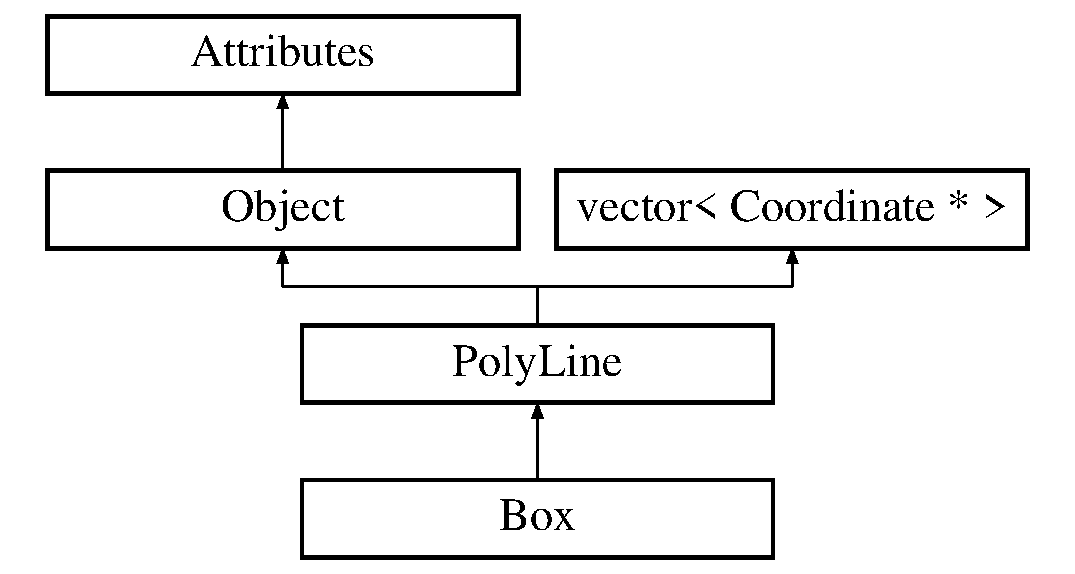
\includegraphics[height=4cm]{classBox}
\end{center}
\end{figure}
\subsection*{Public Methods}
\begin{CompactItemize}
\item 
{\bf Box} ()
\item 
{\bf Box} ({\bf Coordinate} $\ast$coordinate1, {\bf Coordinate} $\ast$coordinate2)
\item 
{\bf $\sim$Box} ()
\end{CompactItemize}


\subsection{Detailed Description}
This class handles box objects. This class is derived from {\bf Poly\-Line} {\rm (p.\,\pageref{classPolyLine})}. \begin{Desc}
\item[Author: ]\par
Anthony Liekens \end{Desc}




\subsection{Constructor \& Destructor Documentation}
\index{Box@{Box}!Box@{Box}}
\index{Box@{Box}!Box@{Box}}
\subsubsection{\setlength{\rightskip}{0pt plus 5cm}Box::Box ()}\label{classBox_a0}


Constructor. Constructs a box object. \index{Box@{Box}!Box@{Box}}
\index{Box@{Box}!Box@{Box}}
\subsubsection{\setlength{\rightskip}{0pt plus 5cm}Box::Box ({\bf Coordinate} $\ast$ {\em coordinate1}, {\bf Coordinate} $\ast$ {\em coordinate2})}\label{classBox_a1}


Constructor. Constructs a box object. \begin{Desc}
\item[Parameters: ]\par
\begin{description}
\item[{\em 
coordinate1}]One corner of the box \item[{\em 
coordinate2}]Opposite corner of the box \end{description}
\end{Desc}
\index{Box@{Box}!~Box@{$\sim$Box}}
\index{~Box@{$\sim$Box}!Box@{Box}}
\subsubsection{\setlength{\rightskip}{0pt plus 5cm}Box::$\sim$Box ()}\label{classBox_a2}


Destructor. Destructs a box object. 

The documentation for this class was generated from the following files:\begin{CompactItemize}
\item 
{\bf box.h}\item 
{\bf box.cpp}\end{CompactItemize}

\section{Coordinate Class Reference}
\label{classCoordinate}\index{Coordinate@{Coordinate}}
{\tt \#include $<$coordinate.h$>$}

Inheritance diagram for Coordinate::\begin{figure}[H]
\begin{center}
\leavevmode
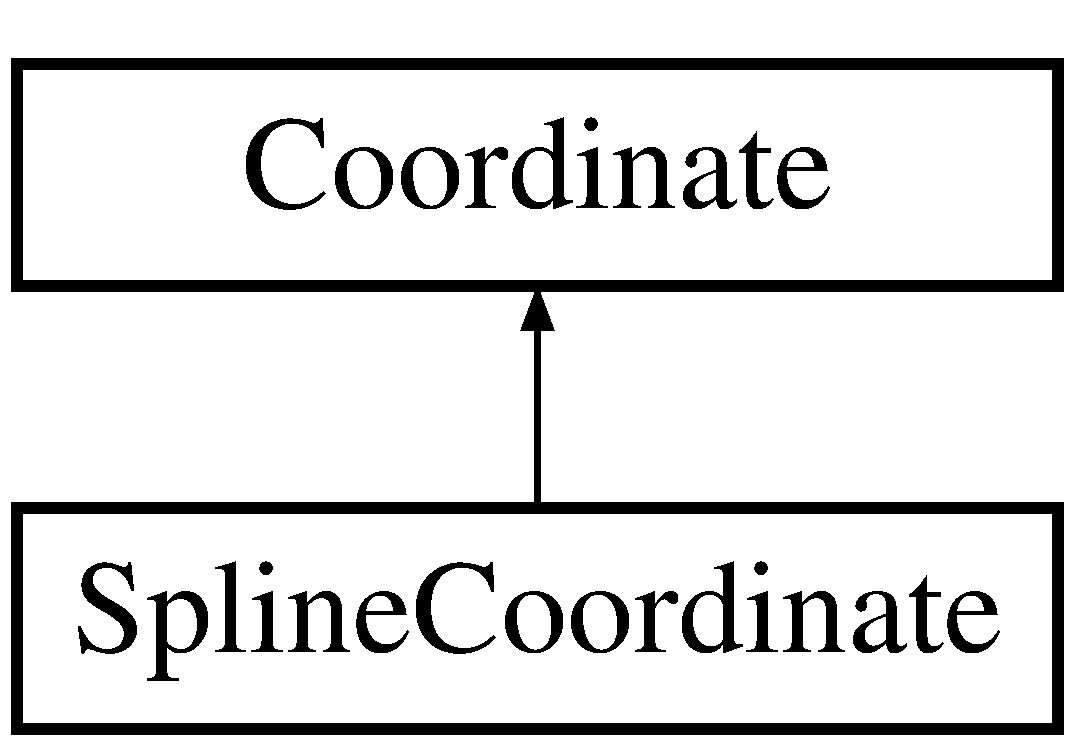
\includegraphics[height=2cm]{classCoordinate}
\end{center}
\end{figure}
\subsection*{Public Methods}
\begin{CompactItemize}
\item 
{\bf Coordinate} ()
\item 
{\bf Coordinate} (double {\bf x}, double {\bf y})
\item 
{\bf $\sim$Coordinate} ()
\item 
void {\bf set\-X} (double {\bf x})
\item 
void {\bf set\-Y} (double {\bf y})
\item 
double {\bf get\-X} ()
\item 
double {\bf get\-Y} ()
\item 
double {\bf distance} (Coordinate $\ast$c)
\item 
void {\bf write} (std::ostream \&stream) const
\end{CompactItemize}
\subsection*{Protected Attributes}
\begin{CompactItemize}
\item 
double {\bf x}
\item 
double {\bf y}
\end{CompactItemize}


\subsection{Detailed Description}
This class handles coordinates. Remember that computers use coordinate systems that are upside-down. This means that the origin of the coordinate system lays in the top-left corner, so the Y axis is upside-down... You will notice that a lot of objects use pointers to Coordinates in constructors, etc. This is because the library needs to be generic, so you can use inherited Coordinates as Coordinates too (for example {\bf Spline\-Coordinate} {\rm (p.\,\pageref{classSplineCoordinate})} instances). \begin{Desc}
\item[Author: ]\par
Anthony Liekens \end{Desc}




\subsection{Constructor \& Destructor Documentation}
\index{Coordinate@{Coordinate}!Coordinate@{Coordinate}}
\index{Coordinate@{Coordinate}!Coordinate@{Coordinate}}
\subsubsection{\setlength{\rightskip}{0pt plus 5cm}Coordinate::Coordinate ()}\label{classCoordinate_a0}


Constructor. Constructs a coordinate. \index{Coordinate@{Coordinate}!Coordinate@{Coordinate}}
\index{Coordinate@{Coordinate}!Coordinate@{Coordinate}}
\subsubsection{\setlength{\rightskip}{0pt plus 5cm}Coordinate::Coordinate (double {\em x}, double {\em y})}\label{classCoordinate_a1}


Constructor. Constructs a coordinate. \begin{Desc}
\item[Parameters: ]\par
\begin{description}
\item[{\em 
x}]Integer X-axis value of the coordinate (0 = leftmost point) \item[{\em 
y}]Integer Y-axis value of the coordinate (0 = top) \end{description}
\end{Desc}
\index{Coordinate@{Coordinate}!~Coordinate@{$\sim$Coordinate}}
\index{~Coordinate@{$\sim$Coordinate}!Coordinate@{Coordinate}}
\subsubsection{\setlength{\rightskip}{0pt plus 5cm}Coordinate::$\sim$Coordinate ()}\label{classCoordinate_a2}


Destructor. Destructs a coordinate. 

\subsection{Member Function Documentation}
\index{Coordinate@{Coordinate}!distance@{distance}}
\index{distance@{distance}!Coordinate@{Coordinate}}
\subsubsection{\setlength{\rightskip}{0pt plus 5cm}double Coordinate::distance (Coordinate $\ast$ {\em c})\hspace{0.3cm}{\tt  [inline]}}\label{classCoordinate_a7}


Returns the distance between this coordinate and another point. \begin{Desc}
\item[Parameters: ]\par
\begin{description}
\item[{\em 
c}]Coordinate of that other point \end{description}
\end{Desc}
\begin{Desc}
\item[Returns: ]\par
int \end{Desc}
\index{Coordinate@{Coordinate}!getX@{getX}}
\index{getX@{getX}!Coordinate@{Coordinate}}
\subsubsection{\setlength{\rightskip}{0pt plus 5cm}double Coordinate::get\-X ()\hspace{0.3cm}{\tt  [inline]}}\label{classCoordinate_a5}


Returns the X-axis value of the coordinate. \begin{Desc}
\item[Returns: ]\par
double \end{Desc}
\index{Coordinate@{Coordinate}!getY@{getY}}
\index{getY@{getY}!Coordinate@{Coordinate}}
\subsubsection{\setlength{\rightskip}{0pt plus 5cm}double Coordinate::get\-Y ()\hspace{0.3cm}{\tt  [inline]}}\label{classCoordinate_a6}


Returns the Y-axis value of the coordinate. \begin{Desc}
\item[Returns: ]\par
double \end{Desc}
\index{Coordinate@{Coordinate}!setX@{setX}}
\index{setX@{setX}!Coordinate@{Coordinate}}
\subsubsection{\setlength{\rightskip}{0pt plus 5cm}void Coordinate::set\-X (double {\em x})\hspace{0.3cm}{\tt  [inline]}}\label{classCoordinate_a3}


Set the X-axis value. \begin{Desc}
\item[Parameters: ]\par
\begin{description}
\item[{\em 
x}]double value \end{description}
\end{Desc}
\begin{Desc}
\item[Returns: ]\par
void \end{Desc}
\index{Coordinate@{Coordinate}!setY@{setY}}
\index{setY@{setY}!Coordinate@{Coordinate}}
\subsubsection{\setlength{\rightskip}{0pt plus 5cm}void Coordinate::set\-Y (double {\em y})\hspace{0.3cm}{\tt  [inline]}}\label{classCoordinate_a4}


Set the Y-axis value. \begin{Desc}
\item[Parameters: ]\par
\begin{description}
\item[{\em 
y}]double value \end{description}
\end{Desc}
\begin{Desc}
\item[Returns: ]\par
void \end{Desc}
\index{Coordinate@{Coordinate}!write@{write}}
\index{write@{write}!Coordinate@{Coordinate}}
\subsubsection{\setlength{\rightskip}{0pt plus 5cm}void Coordinate::write (std::ostream \& {\em stream}) const}\label{classCoordinate_a8}


Write the coordinate object to a given outstream. \begin{Desc}
\item[Parameters: ]\par
\begin{description}
\item[{\em 
stream}]output stream \end{description}
\end{Desc}
\begin{Desc}
\item[Returns: ]\par
void \end{Desc}


\subsection{Member Data Documentation}
\index{Coordinate@{Coordinate}!x@{x}}
\index{x@{x}!Coordinate@{Coordinate}}
\subsubsection{\setlength{\rightskip}{0pt plus 5cm}double Coordinate::x\hspace{0.3cm}{\tt  [protected]}}\label{classCoordinate_n0}


\index{Coordinate@{Coordinate}!y@{y}}
\index{y@{y}!Coordinate@{Coordinate}}
\subsubsection{\setlength{\rightskip}{0pt plus 5cm}double Coordinate::y\hspace{0.3cm}{\tt  [protected]}}\label{classCoordinate_n1}




The documentation for this class was generated from the following files:\begin{CompactItemize}
\item 
{\bf coordinate.h}\item 
{\bf coordinate.cpp}\end{CompactItemize}

\section{Coordinate3D Class Reference}
\label{classCoordinate3D}\index{Coordinate3D@{Coordinate3D}}
{\tt \#include $<$coordinate3d.h$>$}

\subsection*{Public Methods}
\begin{CompactItemize}
\item 
{\bf Coordinate3D} ()
\item 
{\bf Coordinate3D} (double {\bf x}, double {\bf y}, double {\bf z})
\item 
{\bf $\sim$Coordinate3D} ()
\item 
void {\bf set\-X} (double {\bf x})
\item 
void {\bf set\-Y} (double {\bf y})
\item 
void {\bf set\-Z} (double {\bf z})
\item 
double {\bf get\-X} ()
\item 
double {\bf get\-Y} ()
\item 
double {\bf get\-Z} ()
\item 
double {\bf distance} (Coordinate3D $\ast$c)
\item 
{\bf Coordinate} $\ast$ {\bf projection} (double x\-Offset, double y\-Offset, double scale, double distance)
\item 
void {\bf apply\-Matrix} ({\bf Matrix}$<$ double $>$ $\ast$)
\item 
void {\bf translate} (Coordinate3D $\ast$)
\item 
void {\bf write} (std::ostream \&stream) const
\end{CompactItemize}
\subsection*{Protected Attributes}
\begin{CompactItemize}
\item 
double {\bf x}
\item 
double {\bf y}
\item 
double {\bf z}
\end{CompactItemize}


\subsection{Detailed Description}
This class handles coordinates. Remember that computers use coordinate systems that are upside-down. This means that the origin of the coordinate system lays in the top-left corner, so the Y axis is upside-down... You will notice that a lot of objects use pointers to Coordinates in constructors, etc. This is because the library needs to be generic, so you can use inherited Coordinates as Coordinates too (for example {\bf Spline\-Coordinate} {\rm (p.\,\pageref{classSplineCoordinate})} instances). \begin{Desc}
\item[Author: ]\par
Anthony Liekens \end{Desc}




\subsection{Constructor \& Destructor Documentation}
\index{Coordinate3D@{Coordinate3D}!Coordinate3D@{Coordinate3D}}
\index{Coordinate3D@{Coordinate3D}!Coordinate3D@{Coordinate3D}}
\subsubsection{\setlength{\rightskip}{0pt plus 5cm}Coordinate3D::Coordinate3D ()}\label{classCoordinate3D_a0}


Constructor. Constructs a coordinate. \index{Coordinate3D@{Coordinate3D}!Coordinate3D@{Coordinate3D}}
\index{Coordinate3D@{Coordinate3D}!Coordinate3D@{Coordinate3D}}
\subsubsection{\setlength{\rightskip}{0pt plus 5cm}Coordinate3D::Coordinate3D (double {\em x}, double {\em y}, double {\em z})}\label{classCoordinate3D_a1}


Constructor. Constructs a coordinate. \begin{Desc}
\item[Parameters: ]\par
\begin{description}
\item[{\em 
x}]Integer X-axis value of the coordinate (0 = leftmost point) \item[{\em 
y}]Integer Y-axis value of the coordinate (0 = top) \end{description}
\end{Desc}
\index{Coordinate3D@{Coordinate3D}!~Coordinate3D@{$\sim$Coordinate3D}}
\index{~Coordinate3D@{$\sim$Coordinate3D}!Coordinate3D@{Coordinate3D}}
\subsubsection{\setlength{\rightskip}{0pt plus 5cm}Coordinate3D::$\sim$Coordinate3D ()}\label{classCoordinate3D_a2}


Destructor. Destructs a coordinate. 

\subsection{Member Function Documentation}
\index{Coordinate3D@{Coordinate3D}!applyMatrix@{applyMatrix}}
\index{applyMatrix@{applyMatrix}!Coordinate3D@{Coordinate3D}}
\subsubsection{\setlength{\rightskip}{0pt plus 5cm}void Coordinate3D::apply\-Matrix ({\bf Matrix}$<$ double $>$ $\ast$)}\label{classCoordinate3D_a11}


\index{Coordinate3D@{Coordinate3D}!distance@{distance}}
\index{distance@{distance}!Coordinate3D@{Coordinate3D}}
\subsubsection{\setlength{\rightskip}{0pt plus 5cm}double Coordinate3D::distance (Coordinate3D $\ast$ {\em c})\hspace{0.3cm}{\tt  [inline]}}\label{classCoordinate3D_a9}


Returns the distance between this coordinate and another point. \begin{Desc}
\item[Parameters: ]\par
\begin{description}
\item[{\em 
c}]Coordinate3D of that other point \end{description}
\end{Desc}
\begin{Desc}
\item[Returns: ]\par
double \end{Desc}
\index{Coordinate3D@{Coordinate3D}!getX@{getX}}
\index{getX@{getX}!Coordinate3D@{Coordinate3D}}
\subsubsection{\setlength{\rightskip}{0pt plus 5cm}double Coordinate3D::get\-X ()\hspace{0.3cm}{\tt  [inline]}}\label{classCoordinate3D_a6}


Returns the X-axis value of the coordinate. \begin{Desc}
\item[Returns: ]\par
double \end{Desc}
\index{Coordinate3D@{Coordinate3D}!getY@{getY}}
\index{getY@{getY}!Coordinate3D@{Coordinate3D}}
\subsubsection{\setlength{\rightskip}{0pt plus 5cm}double Coordinate3D::get\-Y ()\hspace{0.3cm}{\tt  [inline]}}\label{classCoordinate3D_a7}


Returns the Y-axis value of the coordinate. \begin{Desc}
\item[Returns: ]\par
double \end{Desc}
\index{Coordinate3D@{Coordinate3D}!getZ@{getZ}}
\index{getZ@{getZ}!Coordinate3D@{Coordinate3D}}
\subsubsection{\setlength{\rightskip}{0pt plus 5cm}double Coordinate3D::get\-Z ()\hspace{0.3cm}{\tt  [inline]}}\label{classCoordinate3D_a8}


Returns the Y-axis value of the coordinate. \begin{Desc}
\item[Returns: ]\par
double \end{Desc}
\index{Coordinate3D@{Coordinate3D}!projection@{projection}}
\index{projection@{projection}!Coordinate3D@{Coordinate3D}}
\subsubsection{\setlength{\rightskip}{0pt plus 5cm}{\bf Coordinate} $\ast$ Coordinate3D::projection (double {\em x\-Offset}, double {\em y\-Offset}, double {\em scale}, double {\em distance})}\label{classCoordinate3D_a10}


\index{Coordinate3D@{Coordinate3D}!setX@{setX}}
\index{setX@{setX}!Coordinate3D@{Coordinate3D}}
\subsubsection{\setlength{\rightskip}{0pt plus 5cm}void Coordinate3D::set\-X (double {\em x})\hspace{0.3cm}{\tt  [inline]}}\label{classCoordinate3D_a3}


Set the X-axis value. \begin{Desc}
\item[Parameters: ]\par
\begin{description}
\item[{\em 
x}]double value \end{description}
\end{Desc}
\begin{Desc}
\item[Returns: ]\par
void \end{Desc}
\index{Coordinate3D@{Coordinate3D}!setY@{setY}}
\index{setY@{setY}!Coordinate3D@{Coordinate3D}}
\subsubsection{\setlength{\rightskip}{0pt plus 5cm}void Coordinate3D::set\-Y (double {\em y})\hspace{0.3cm}{\tt  [inline]}}\label{classCoordinate3D_a4}


Set the Y-axis value. \begin{Desc}
\item[Parameters: ]\par
\begin{description}
\item[{\em 
y}]double value \end{description}
\end{Desc}
\begin{Desc}
\item[Returns: ]\par
void \end{Desc}
\index{Coordinate3D@{Coordinate3D}!setZ@{setZ}}
\index{setZ@{setZ}!Coordinate3D@{Coordinate3D}}
\subsubsection{\setlength{\rightskip}{0pt plus 5cm}void Coordinate3D::set\-Z (double {\em z})\hspace{0.3cm}{\tt  [inline]}}\label{classCoordinate3D_a5}


Set the Z-axis value. \begin{Desc}
\item[Parameters: ]\par
\begin{description}
\item[{\em 
z}]double value \end{description}
\end{Desc}
\begin{Desc}
\item[Returns: ]\par
void \end{Desc}
\index{Coordinate3D@{Coordinate3D}!translate@{translate}}
\index{translate@{translate}!Coordinate3D@{Coordinate3D}}
\subsubsection{\setlength{\rightskip}{0pt plus 5cm}void Coordinate3D::translate (Coordinate3D $\ast$)}\label{classCoordinate3D_a12}


\index{Coordinate3D@{Coordinate3D}!write@{write}}
\index{write@{write}!Coordinate3D@{Coordinate3D}}
\subsubsection{\setlength{\rightskip}{0pt plus 5cm}void Coordinate3D::write (std::ostream \& {\em stream}) const}\label{classCoordinate3D_a13}


Write the coordinate object to a given outstream. \begin{Desc}
\item[Parameters: ]\par
\begin{description}
\item[{\em 
stream}]output stream \end{description}
\end{Desc}
\begin{Desc}
\item[Returns: ]\par
void \end{Desc}


\subsection{Member Data Documentation}
\index{Coordinate3D@{Coordinate3D}!x@{x}}
\index{x@{x}!Coordinate3D@{Coordinate3D}}
\subsubsection{\setlength{\rightskip}{0pt plus 5cm}double Coordinate3D::x\hspace{0.3cm}{\tt  [protected]}}\label{classCoordinate3D_n0}


\index{Coordinate3D@{Coordinate3D}!y@{y}}
\index{y@{y}!Coordinate3D@{Coordinate3D}}
\subsubsection{\setlength{\rightskip}{0pt plus 5cm}double Coordinate3D::y\hspace{0.3cm}{\tt  [protected]}}\label{classCoordinate3D_n1}


\index{Coordinate3D@{Coordinate3D}!z@{z}}
\index{z@{z}!Coordinate3D@{Coordinate3D}}
\subsubsection{\setlength{\rightskip}{0pt plus 5cm}double Coordinate3D::z\hspace{0.3cm}{\tt  [protected]}}\label{classCoordinate3D_n2}




The documentation for this class was generated from the following files:\begin{CompactItemize}
\item 
{\bf coordinate3d.h}\item 
{\bf coordinate3d.cpp}\end{CompactItemize}

\section{Diameter\-Circle Class Reference}
\label{classDiameterCircle}\index{DiameterCircle@{DiameterCircle}}
{\tt \#include $<$diametercircle.h$>$}

Inheritance diagram for Diameter\-Circle::\begin{figure}[H]
\begin{center}
\leavevmode
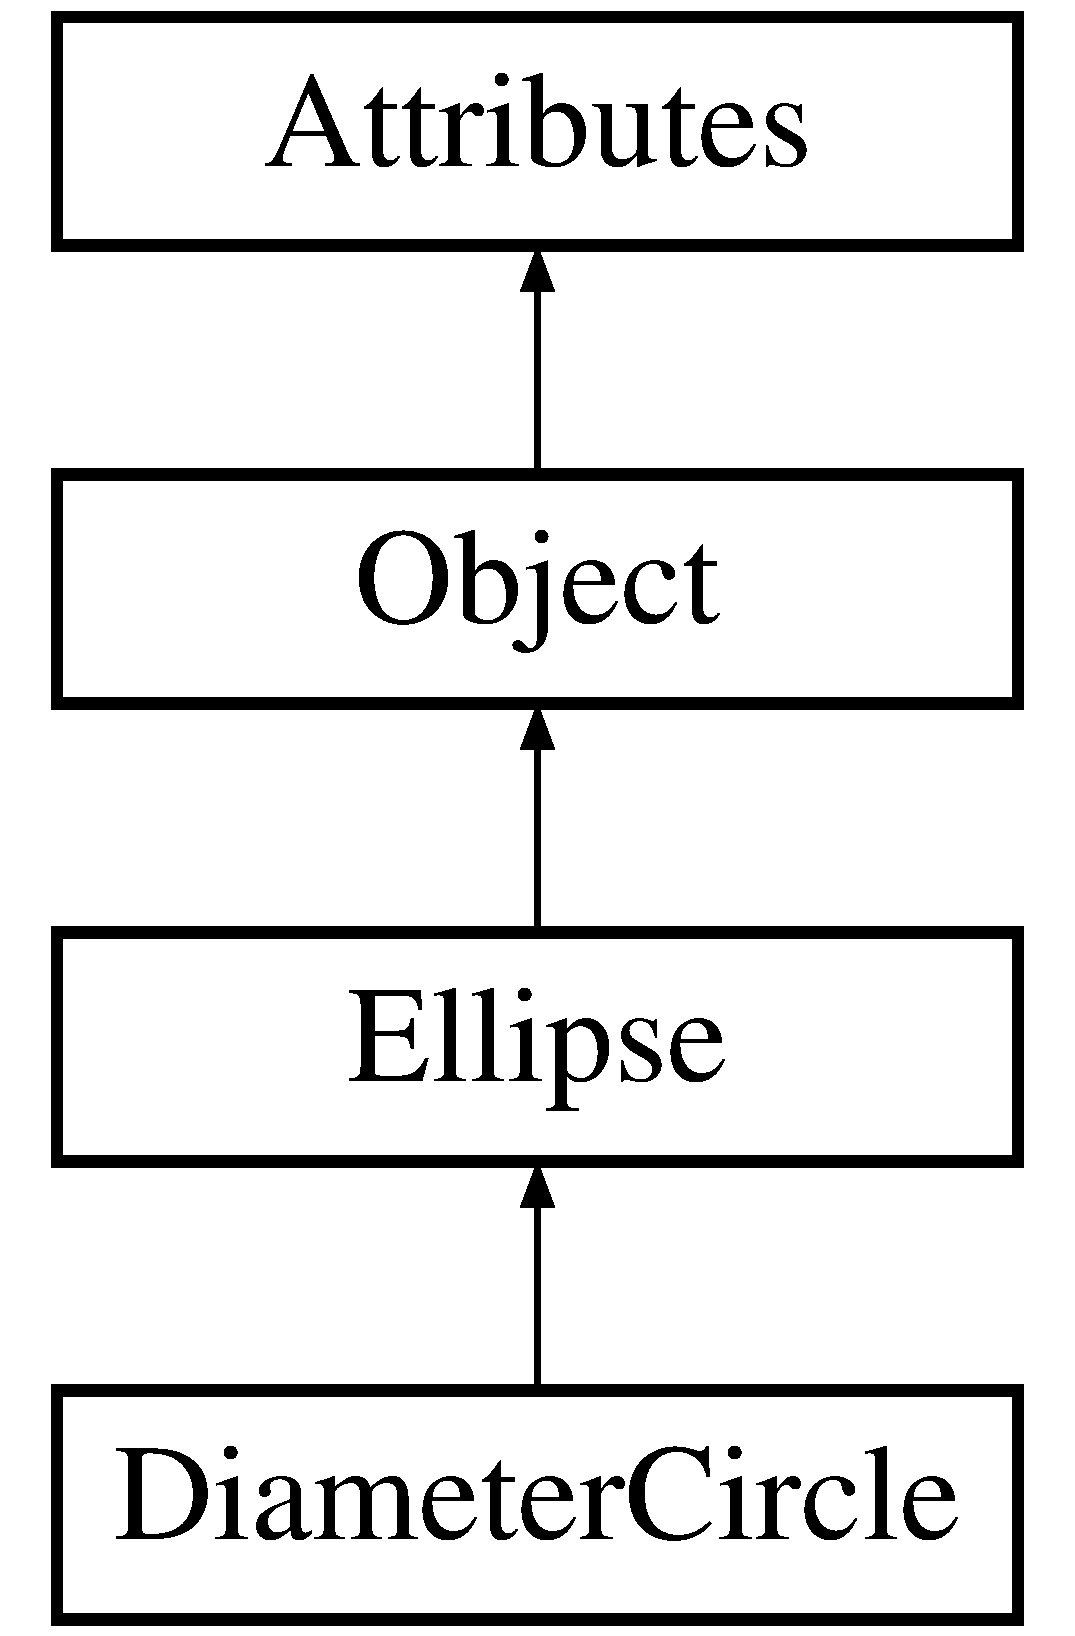
\includegraphics[height=4cm]{classDiameterCircle}
\end{center}
\end{figure}
\subsection*{Public Methods}
\begin{CompactItemize}
\item 
{\bf Diameter\-Circle} ()
\item 
{\bf Diameter\-Circle} ({\bf Coordinate} $\ast$, {\bf Coordinate} $\ast$)
\item 
{\bf $\sim$Diameter\-Circle} ()
\end{CompactItemize}


\subsection{Detailed Description}
This class handles circles defined by their diameter. This class is derived from {\bf Ellipse} {\rm (p.\,\pageref{classEllipse})}. \begin{Desc}
\item[Author: ]\par
Anthony Liekens \end{Desc}




\subsection{Constructor \& Destructor Documentation}
\index{DiameterCircle@{Diameter\-Circle}!DiameterCircle@{DiameterCircle}}
\index{DiameterCircle@{DiameterCircle}!DiameterCircle@{Diameter\-Circle}}
\subsubsection{\setlength{\rightskip}{0pt plus 5cm}Diameter\-Circle::Diameter\-Circle ()}\label{classDiameterCircle_a0}


\index{DiameterCircle@{Diameter\-Circle}!DiameterCircle@{DiameterCircle}}
\index{DiameterCircle@{DiameterCircle}!DiameterCircle@{Diameter\-Circle}}
\subsubsection{\setlength{\rightskip}{0pt plus 5cm}Diameter\-Circle::Diameter\-Circle ({\bf Coordinate} $\ast$, {\bf Coordinate} $\ast$)}\label{classDiameterCircle_a1}


\index{DiameterCircle@{Diameter\-Circle}!~DiameterCircle@{$\sim$DiameterCircle}}
\index{~DiameterCircle@{$\sim$DiameterCircle}!DiameterCircle@{Diameter\-Circle}}
\subsubsection{\setlength{\rightskip}{0pt plus 5cm}Diameter\-Circle::$\sim$Diameter\-Circle ()}\label{classDiameterCircle_a2}




The documentation for this class was generated from the following files:\begin{CompactItemize}
\item 
{\bf diametercircle.h}\item 
{\bf diametercircle.cpp}\end{CompactItemize}

\section{Diameter\-Ellipse Class Reference}
\label{classDiameterEllipse}\index{DiameterEllipse@{DiameterEllipse}}
{\tt \#include $<$diameterellipse.h$>$}

Inheritance diagram for Diameter\-Ellipse::\begin{figure}[H]
\begin{center}
\leavevmode
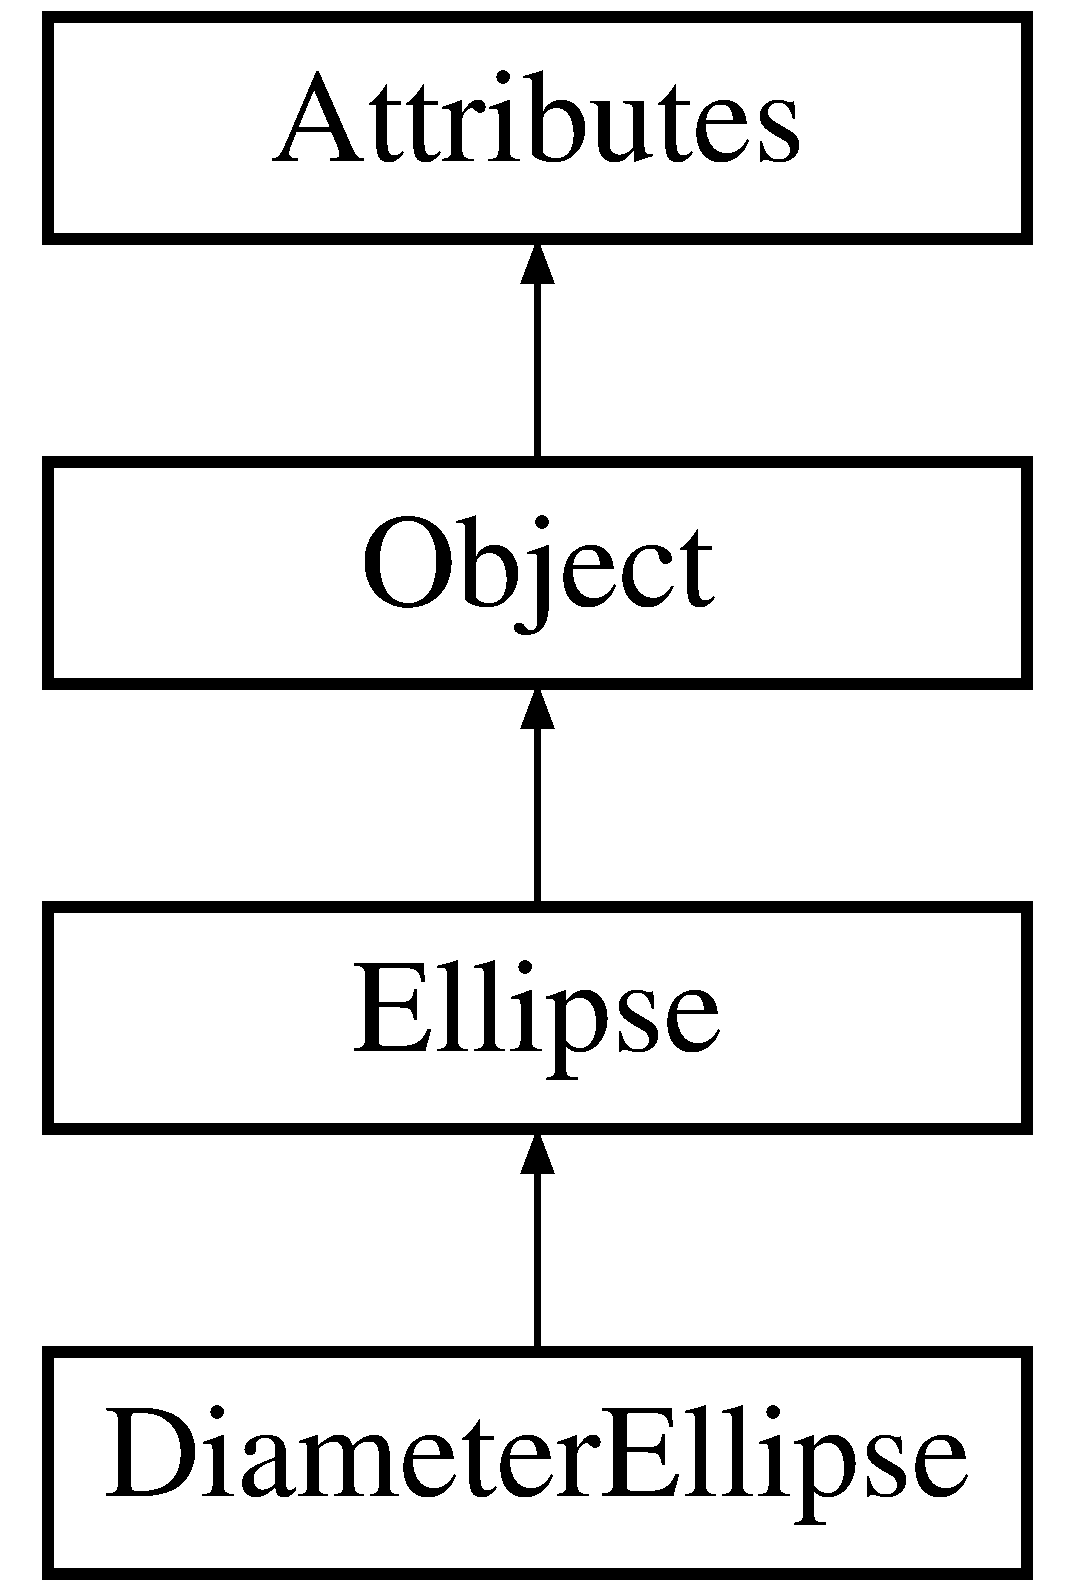
\includegraphics[height=4cm]{classDiameterEllipse}
\end{center}
\end{figure}
\subsection*{Public Methods}
\begin{CompactItemize}
\item 
{\bf Diameter\-Ellipse} ()
\item 
{\bf Diameter\-Ellipse} ({\bf Coordinate} $\ast$, {\bf Coordinate} $\ast$)
\item 
{\bf $\sim$Diameter\-Ellipse} ()
\end{CompactItemize}


\subsection{Detailed Description}
This class handles ellipses defined by their bounding box. This class is derived from {\bf Ellipse} {\rm (p.\,\pageref{classEllipse})}. \begin{Desc}
\item[Author: ]\par
Anthony Liekens \end{Desc}




\subsection{Constructor \& Destructor Documentation}
\index{DiameterEllipse@{Diameter\-Ellipse}!DiameterEllipse@{DiameterEllipse}}
\index{DiameterEllipse@{DiameterEllipse}!DiameterEllipse@{Diameter\-Ellipse}}
\subsubsection{\setlength{\rightskip}{0pt plus 5cm}Diameter\-Ellipse::Diameter\-Ellipse ()}\label{classDiameterEllipse_a0}


\index{DiameterEllipse@{Diameter\-Ellipse}!DiameterEllipse@{DiameterEllipse}}
\index{DiameterEllipse@{DiameterEllipse}!DiameterEllipse@{Diameter\-Ellipse}}
\subsubsection{\setlength{\rightskip}{0pt plus 5cm}Diameter\-Ellipse::Diameter\-Ellipse ({\bf Coordinate} $\ast$, {\bf Coordinate} $\ast$)}\label{classDiameterEllipse_a1}


\index{DiameterEllipse@{Diameter\-Ellipse}!~DiameterEllipse@{$\sim$DiameterEllipse}}
\index{~DiameterEllipse@{$\sim$DiameterEllipse}!DiameterEllipse@{Diameter\-Ellipse}}
\subsubsection{\setlength{\rightskip}{0pt plus 5cm}Diameter\-Ellipse::$\sim$Diameter\-Ellipse ()}\label{classDiameterEllipse_a2}




The documentation for this class was generated from the following files:\begin{CompactItemize}
\item 
{\bf diameterellipse.h}\item 
{\bf diameterellipse.cpp}\end{CompactItemize}

\section{Ellipse Class Reference}
\label{classEllipse}\index{Ellipse@{Ellipse}}
{\tt \#include $<$ellipse.h$>$}

Inheritance diagram for Ellipse::\begin{figure}[H]
\begin{center}
\leavevmode
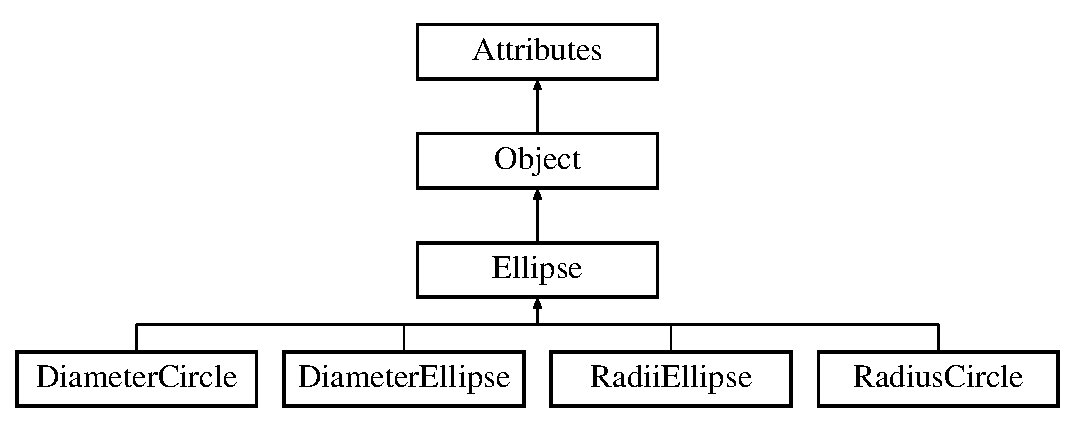
\includegraphics[height=4cm]{classEllipse}
\end{center}
\end{figure}
\subsection*{Public Methods}
\begin{CompactItemize}
\item 
{\bf Ellipse} ()
\item 
{\bf $\sim$Ellipse} ()
\item 
int {\bf get\-Sub\-Type} ()
\item 
void {\bf set\-Angle} (float {\bf angle})
\item 
float {\bf get\-Angle} ()
\item 
void {\bf set\-Center} ({\bf Coordinate} $\ast${\bf center})
\item 
{\bf Coordinate} $\ast$ {\bf get\-Center} ()
\item 
void {\bf set\-Radii} ({\bf Coordinate} $\ast${\bf radius})
\item 
{\bf Coordinate} $\ast$ {\bf get\-Radii} ()
\item 
void {\bf set\-Start} ({\bf Coordinate} $\ast${\bf start})
\item 
{\bf Coordinate} $\ast$ {\bf get\-Start} ()
\item 
void {\bf set\-End} ({\bf Coordinate} $\ast${\bf end})
\item 
{\bf Coordinate} $\ast$ {\bf get\-End} ()
\item 
void {\bf write} (std::ostream \&stream) const
\end{CompactItemize}
\subsection*{Protected Methods}
\begin{CompactItemize}
\item 
void {\bf set\-Sub\-Type} (int {\bf sub\-Type})
\end{CompactItemize}
\subsection*{Protected Attributes}
\begin{CompactItemize}
\item 
int {\bf sub\-Type}
\item 
int {\bf direction}
\item 
float {\bf angle}
\item 
{\bf Coordinate} $\ast$ {\bf center}
\item 
{\bf Coordinate} $\ast$ {\bf radii}
\item 
{\bf Coordinate} $\ast$ {\bf start}
\item 
{\bf Coordinate} $\ast$ {\bf end}
\end{CompactItemize}


\subsection{Detailed Description}
This class handles ellipses and circles. This class is derived from {\bf Object} {\rm (p.\,\pageref{classObject})}. \begin{Desc}
\item[Author: ]\par
Anthony Liekens \end{Desc}




\subsection{Constructor \& Destructor Documentation}
\index{Ellipse@{Ellipse}!Ellipse@{Ellipse}}
\index{Ellipse@{Ellipse}!Ellipse@{Ellipse}}
\subsubsection{\setlength{\rightskip}{0pt plus 5cm}Ellipse::Ellipse ()}\label{classEllipse_a0}


\index{Ellipse@{Ellipse}!~Ellipse@{$\sim$Ellipse}}
\index{~Ellipse@{$\sim$Ellipse}!Ellipse@{Ellipse}}
\subsubsection{\setlength{\rightskip}{0pt plus 5cm}Ellipse::$\sim$Ellipse ()}\label{classEllipse_a1}




\subsection{Member Function Documentation}
\index{Ellipse@{Ellipse}!getAngle@{getAngle}}
\index{getAngle@{getAngle}!Ellipse@{Ellipse}}
\subsubsection{\setlength{\rightskip}{0pt plus 5cm}float Ellipse::get\-Angle ()\hspace{0.3cm}{\tt  [inline]}}\label{classEllipse_a4}


Returns the angle. \begin{Desc}
\item[Returns: ]\par
float \end{Desc}


Reimplemented from {\bf Attributes} {\rm (p.\,\pageref{classAttributes_a39})}.\index{Ellipse@{Ellipse}!getCenter@{getCenter}}
\index{getCenter@{getCenter}!Ellipse@{Ellipse}}
\subsubsection{\setlength{\rightskip}{0pt plus 5cm}{\bf Coordinate}$\ast$ Ellipse::get\-Center ()\hspace{0.3cm}{\tt  [inline]}}\label{classEllipse_a6}


\index{Ellipse@{Ellipse}!getEnd@{getEnd}}
\index{getEnd@{getEnd}!Ellipse@{Ellipse}}
\subsubsection{\setlength{\rightskip}{0pt plus 5cm}{\bf Coordinate}$\ast$ Ellipse::get\-End ()\hspace{0.3cm}{\tt  [inline]}}\label{classEllipse_a12}


\index{Ellipse@{Ellipse}!getRadii@{getRadii}}
\index{getRadii@{getRadii}!Ellipse@{Ellipse}}
\subsubsection{\setlength{\rightskip}{0pt plus 5cm}{\bf Coordinate}$\ast$ Ellipse::get\-Radii ()\hspace{0.3cm}{\tt  [inline]}}\label{classEllipse_a8}


\index{Ellipse@{Ellipse}!getStart@{getStart}}
\index{getStart@{getStart}!Ellipse@{Ellipse}}
\subsubsection{\setlength{\rightskip}{0pt plus 5cm}{\bf Coordinate}$\ast$ Ellipse::get\-Start ()\hspace{0.3cm}{\tt  [inline]}}\label{classEllipse_a10}


\index{Ellipse@{Ellipse}!getSubType@{getSubType}}
\index{getSubType@{getSubType}!Ellipse@{Ellipse}}
\subsubsection{\setlength{\rightskip}{0pt plus 5cm}int Ellipse::get\-Sub\-Type ()\hspace{0.3cm}{\tt  [inline]}}\label{classEllipse_a2}


\index{Ellipse@{Ellipse}!setAngle@{setAngle}}
\index{setAngle@{setAngle}!Ellipse@{Ellipse}}
\subsubsection{\setlength{\rightskip}{0pt plus 5cm}void Ellipse::set\-Angle (float {\em angle})\hspace{0.3cm}{\tt  [inline]}}\label{classEllipse_a3}


Set the angle. \begin{Desc}
\item[Parameters: ]\par
\begin{description}
\item[{\em 
angle}]float value \end{description}
\end{Desc}
\begin{Desc}
\item[Returns: ]\par
void \end{Desc}


Reimplemented from {\bf Attributes} {\rm (p.\,\pageref{classAttributes_a17})}.\index{Ellipse@{Ellipse}!setCenter@{setCenter}}
\index{setCenter@{setCenter}!Ellipse@{Ellipse}}
\subsubsection{\setlength{\rightskip}{0pt plus 5cm}void Ellipse::set\-Center ({\bf Coordinate} $\ast$ {\em center})\hspace{0.3cm}{\tt  [inline]}}\label{classEllipse_a5}


\index{Ellipse@{Ellipse}!setEnd@{setEnd}}
\index{setEnd@{setEnd}!Ellipse@{Ellipse}}
\subsubsection{\setlength{\rightskip}{0pt plus 5cm}void Ellipse::set\-End ({\bf Coordinate} $\ast$ {\em end})\hspace{0.3cm}{\tt  [inline]}}\label{classEllipse_a11}


\index{Ellipse@{Ellipse}!setRadii@{setRadii}}
\index{setRadii@{setRadii}!Ellipse@{Ellipse}}
\subsubsection{\setlength{\rightskip}{0pt plus 5cm}void Ellipse::set\-Radii ({\bf Coordinate} $\ast$ {\em radius})\hspace{0.3cm}{\tt  [inline]}}\label{classEllipse_a7}


\index{Ellipse@{Ellipse}!setStart@{setStart}}
\index{setStart@{setStart}!Ellipse@{Ellipse}}
\subsubsection{\setlength{\rightskip}{0pt plus 5cm}void Ellipse::set\-Start ({\bf Coordinate} $\ast$ {\em start})\hspace{0.3cm}{\tt  [inline]}}\label{classEllipse_a9}


\index{Ellipse@{Ellipse}!setSubType@{setSubType}}
\index{setSubType@{setSubType}!Ellipse@{Ellipse}}
\subsubsection{\setlength{\rightskip}{0pt plus 5cm}void Ellipse::set\-Sub\-Type (int {\em sub\-Type})\hspace{0.3cm}{\tt  [inline, protected]}}\label{classEllipse_b0}


\index{Ellipse@{Ellipse}!write@{write}}
\index{write@{write}!Ellipse@{Ellipse}}
\subsubsection{\setlength{\rightskip}{0pt plus 5cm}void Ellipse::write (std::ostream \& {\em stream}) const\hspace{0.3cm}{\tt  [virtual]}}\label{classEllipse_a13}


Write the object to a given outstream. All inherited classes of object should provide this method, since it's called by {\bf Figure} {\rm (p.\,\pageref{classFigure})} (the object container) to output objects to a given stream. \begin{Desc}
\item[Parameters: ]\par
\begin{description}
\item[{\em 
stream}]output stream \end{description}
\end{Desc}
\begin{Desc}
\item[Returns: ]\par
void \end{Desc}


Reimplemented from {\bf Object} {\rm (p.\,\pageref{classObject_a3})}.

\subsection{Member Data Documentation}
\index{Ellipse@{Ellipse}!angle@{angle}}
\index{angle@{angle}!Ellipse@{Ellipse}}
\subsubsection{\setlength{\rightskip}{0pt plus 5cm}float Ellipse::angle\hspace{0.3cm}{\tt  [protected]}}\label{classEllipse_n2}




Reimplemented from {\bf Attributes} {\rm (p.\,\pageref{classAttributes_n13})}.\index{Ellipse@{Ellipse}!center@{center}}
\index{center@{center}!Ellipse@{Ellipse}}
\subsubsection{\setlength{\rightskip}{0pt plus 5cm}{\bf Coordinate}$\ast$ Ellipse::center\hspace{0.3cm}{\tt  [protected]}}\label{classEllipse_n3}


\index{Ellipse@{Ellipse}!direction@{direction}}
\index{direction@{direction}!Ellipse@{Ellipse}}
\subsubsection{\setlength{\rightskip}{0pt plus 5cm}int Ellipse::direction\hspace{0.3cm}{\tt  [protected]}}\label{classEllipse_n1}


\index{Ellipse@{Ellipse}!end@{end}}
\index{end@{end}!Ellipse@{Ellipse}}
\subsubsection{\setlength{\rightskip}{0pt plus 5cm}{\bf Coordinate} $\ast$ Ellipse::end\hspace{0.3cm}{\tt  [protected]}}\label{classEllipse_n6}


\index{Ellipse@{Ellipse}!radii@{radii}}
\index{radii@{radii}!Ellipse@{Ellipse}}
\subsubsection{\setlength{\rightskip}{0pt plus 5cm}{\bf Coordinate}$\ast$ Ellipse::radii\hspace{0.3cm}{\tt  [protected]}}\label{classEllipse_n4}


\index{Ellipse@{Ellipse}!start@{start}}
\index{start@{start}!Ellipse@{Ellipse}}
\subsubsection{\setlength{\rightskip}{0pt plus 5cm}{\bf Coordinate}$\ast$ Ellipse::start\hspace{0.3cm}{\tt  [protected]}}\label{classEllipse_n5}


\index{Ellipse@{Ellipse}!subType@{subType}}
\index{subType@{subType}!Ellipse@{Ellipse}}
\subsubsection{\setlength{\rightskip}{0pt plus 5cm}int Ellipse::sub\-Type\hspace{0.3cm}{\tt  [protected]}}\label{classEllipse_n0}




The documentation for this class was generated from the following files:\begin{CompactItemize}
\item 
{\bf ellipse.h}\item 
{\bf ellipse.cpp}\end{CompactItemize}

\section{Figure Class Reference}
\label{classFigure}\index{Figure@{Figure}}
{\tt \#include $<$figure.h$>$}

Inheritance diagram for Figure::\begin{figure}[H]
\begin{center}
\leavevmode
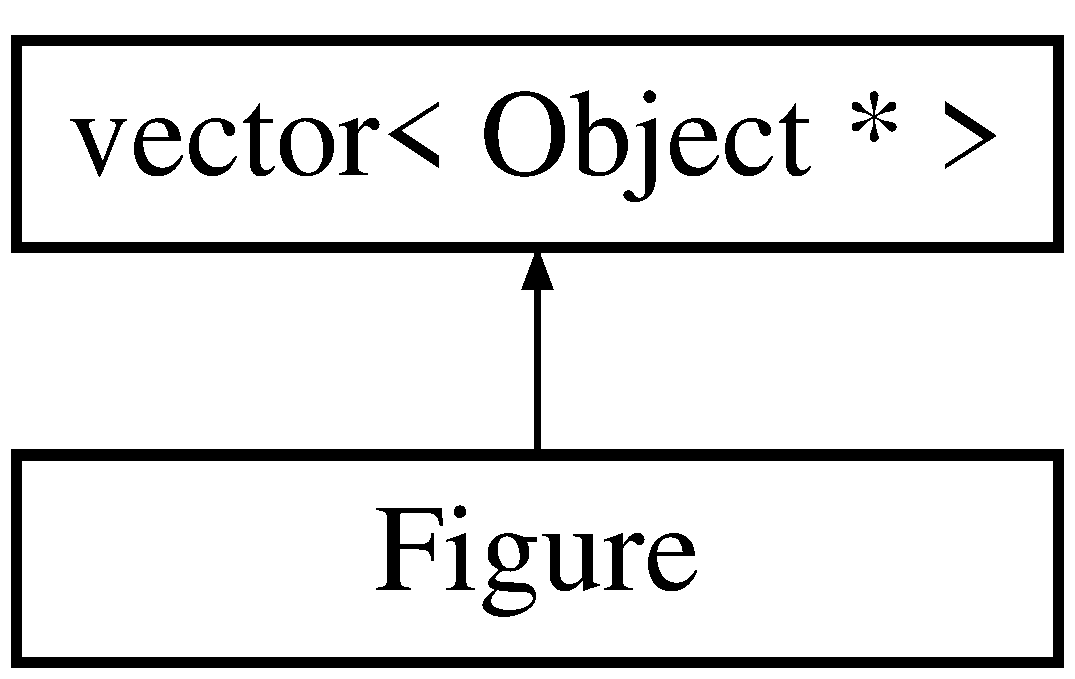
\includegraphics[height=2cm]{classFigure}
\end{center}
\end{figure}
\subsection*{Public Types}
\begin{CompactItemize}
\item 
enum {\bf Orientations} \{ {\bf Landscape} =  0, 
{\bf Portrait} =  1
 \}
\item 
enum {\bf Justifications} \{ {\bf Center} =  0, 
{\bf Flush\-Left} =  1
 \}
\item 
enum {\bf Units} \{ {\bf Metric} =  0, 
{\bf Inches} =  1
 \}
\item 
enum {\bf Papersizes} \{ {\bf Letter} =  0, 
{\bf Legal} =  1, 
{\bf Ledger} =  2, 
{\bf Tabloid} =  3, 
{\bf A} =  4, 
{\bf B} =  5, 
{\bf C} =  6, 
{\bf D} =  7, 
{\bf E} =  8, 
{\bf A4} =  9, 
{\bf A3} =  10, 
{\bf A2} =  11, 
{\bf A1} =  12, 
{\bf A0} =  13, 
{\bf B5} =  14
 \}
\item 
enum {\bf Multiple\-Pages} \{ {\bf Single} =  0, 
{\bf Multiple} =  1
 \}
\end{CompactItemize}
\subsection*{Public Methods}
\begin{CompactItemize}
\item 
{\bf Figure} ()
\item 
{\bf $\sim$Figure} ()
\item 
void {\bf set\-Orientation} ({\bf Orientations} {\bf orientation})
\item 
void {\bf set\-Justification} ({\bf Justifications} {\bf justification})
\item 
void {\bf set\-Units} ({\bf Units} {\bf units})
\item 
void {\bf set\-Papersize} ({\bf Papersizes} {\bf papersize})
\item 
void {\bf set\-Magnification} (float {\bf magnification})
\item 
void {\bf set\-Multiple\-Page} ({\bf Multiple\-Pages} {\bf multiple\-Page})
\item 
void {\bf set\-Transparent\-Color} (int {\bf transparent\-Color})
\item 
void {\bf set\-Resolution} (int {\bf resolution})
\item 
void {\bf set\-Coord\-System} (int {\bf coord\-System})
\item 
{\bf Orientations} {\bf get\-Orientation} ()
\item 
{\bf Justifications} {\bf get\-Justification} ()
\item 
{\bf Units} {\bf get\-Units} ()
\item 
{\bf Papersizes} {\bf get\-Papersize} ()
\item 
float {\bf get\-Magnification} ()
\item 
{\bf Multiple\-Pages} {\bf get\-Multiple\-Page} ()
\item 
int {\bf get\-Transparent\-Color} ()
\item 
int {\bf get\-Resolution} ()
\item 
int {\bf get\-Coord\-System} ()
\item 
void {\bf write} (std::ostream \&stream) const
\item 
void {\bf write} (std::ostream \&stream, {\bf Orientations} orientations) const
\item 
void {\bf write} (std::ostream \&stream, {\bf Justifications} justifications) const
\item 
void {\bf write} (std::ostream \&stream, {\bf Papersizes} paparesizes) const
\item 
void {\bf write} (std::ostream \&stream, {\bf Units} {\bf units}) const
\item 
void {\bf write} (std::ostream \&stream, {\bf Multiple\-Pages} multiplepages) const
\end{CompactItemize}
\subsection*{Private Attributes}
\begin{CompactItemize}
\item 
{\bf Orientations} {\bf orientation}
\item 
{\bf Justifications} {\bf justification}
\item 
{\bf Units} {\bf units}
\item 
{\bf Papersizes} {\bf papersize}
\item 
float {\bf magnification}
\item 
{\bf Multiple\-Pages} {\bf multiple\-Page}
\item 
int {\bf transparent\-Color}
\item 
int {\bf resolution}
\item 
int {\bf coord\-System}
\end{CompactItemize}


\subsection{Detailed Description}
This class handles figures, and can output them in .fig format. \begin{Desc}
\item[Author: ]\par
Anthony Liekens \end{Desc}




\subsection{Member Enumeration Documentation}
\index{Figure@{Figure}!Justifications@{Justifications}}
\index{Justifications@{Justifications}!Figure@{Figure}}
\subsubsection{\setlength{\rightskip}{0pt plus 5cm}enum Figure::Justifications}\label{classFigure_s24}


Enumeration of justifications. The following justifications can be used to set the justification of a figure object : \{$\backslash$tt Center, Flush\-Left\} \begin{Desc}
\item[Enumeration values: ]\par
\begin{description}
\index{Center@{Center}!Figure@{Figure}}\index{Figure@{Figure}!Center@{Center}}\item[{\em 
{\em Center}\label{classFigure_s24s2}
}]\index{FlushLeft@{FlushLeft}!Figure@{Figure}}\index{Figure@{Figure}!FlushLeft@{FlushLeft}}\item[{\em 
{\em Flush\-Left}\label{classFigure_s24s3}
}]\end{description}
\end{Desc}

\index{Figure@{Figure}!MultiplePages@{MultiplePages}}
\index{MultiplePages@{MultiplePages}!Figure@{Figure}}
\subsubsection{\setlength{\rightskip}{0pt plus 5cm}enum Figure::Multiple\-Pages}\label{classFigure_s27}


Enumeration of multiple pages types. The following types can be used to set the multiple page property of a figure object : \{$\backslash$tt Single, Multiple\} \begin{Desc}
\item[Enumeration values: ]\par
\begin{description}
\index{Single@{Single}!Figure@{Figure}}\index{Figure@{Figure}!Single@{Single}}\item[{\em 
{\em Single}\label{classFigure_s27s21}
}]\index{Multiple@{Multiple}!Figure@{Figure}}\index{Figure@{Figure}!Multiple@{Multiple}}\item[{\em 
{\em Multiple}\label{classFigure_s27s22}
}]\end{description}
\end{Desc}

\index{Figure@{Figure}!Orientations@{Orientations}}
\index{Orientations@{Orientations}!Figure@{Figure}}
\subsubsection{\setlength{\rightskip}{0pt plus 5cm}enum Figure::Orientations}\label{classFigure_s23}


Enumeration of orientations. The following orientations can be used to set the orientation of a figure object : \{$\backslash$tt Landscape, Portrait\} \begin{Desc}
\item[Enumeration values: ]\par
\begin{description}
\index{Landscape@{Landscape}!Figure@{Figure}}\index{Figure@{Figure}!Landscape@{Landscape}}\item[{\em 
{\em Landscape}\label{classFigure_s23s0}
}]\index{Portrait@{Portrait}!Figure@{Figure}}\index{Figure@{Figure}!Portrait@{Portrait}}\item[{\em 
{\em Portrait}\label{classFigure_s23s1}
}]\end{description}
\end{Desc}

\index{Figure@{Figure}!Papersizes@{Papersizes}}
\index{Papersizes@{Papersizes}!Figure@{Figure}}
\subsubsection{\setlength{\rightskip}{0pt plus 5cm}enum Figure::Papersizes}\label{classFigure_s26}


Enumeration of papersizes. The following papersizes can be used to set the papersize of a figure object : \{$\backslash$tt Letter, Legal, Ledger, Tabloid, A, B, C, D, E, A4, A3, A2, A1, A0, B5\} \begin{Desc}
\item[Enumeration values: ]\par
\begin{description}
\index{Letter@{Letter}!Figure@{Figure}}\index{Figure@{Figure}!Letter@{Letter}}\item[{\em 
{\em Letter}\label{classFigure_s26s6}
}]\index{Legal@{Legal}!Figure@{Figure}}\index{Figure@{Figure}!Legal@{Legal}}\item[{\em 
{\em Legal}\label{classFigure_s26s7}
}]\index{Ledger@{Ledger}!Figure@{Figure}}\index{Figure@{Figure}!Ledger@{Ledger}}\item[{\em 
{\em Ledger}\label{classFigure_s26s8}
}]\index{Tabloid@{Tabloid}!Figure@{Figure}}\index{Figure@{Figure}!Tabloid@{Tabloid}}\item[{\em 
{\em Tabloid}\label{classFigure_s26s9}
}]\index{A@{A}!Figure@{Figure}}\index{Figure@{Figure}!A@{A}}\item[{\em 
{\em A}\label{classFigure_s26s10}
}]\index{B@{B}!Figure@{Figure}}\index{Figure@{Figure}!B@{B}}\item[{\em 
{\em B}\label{classFigure_s26s11}
}]\index{C@{C}!Figure@{Figure}}\index{Figure@{Figure}!C@{C}}\item[{\em 
{\em C}\label{classFigure_s26s12}
}]\index{D@{D}!Figure@{Figure}}\index{Figure@{Figure}!D@{D}}\item[{\em 
{\em D}\label{classFigure_s26s13}
}]\index{E@{E}!Figure@{Figure}}\index{Figure@{Figure}!E@{E}}\item[{\em 
{\em E}\label{classFigure_s26s14}
}]\index{A4@{A4}!Figure@{Figure}}\index{Figure@{Figure}!A4@{A4}}\item[{\em 
{\em A4}\label{classFigure_s26s15}
}]\index{A3@{A3}!Figure@{Figure}}\index{Figure@{Figure}!A3@{A3}}\item[{\em 
{\em A3}\label{classFigure_s26s16}
}]\index{A2@{A2}!Figure@{Figure}}\index{Figure@{Figure}!A2@{A2}}\item[{\em 
{\em A2}\label{classFigure_s26s17}
}]\index{A1@{A1}!Figure@{Figure}}\index{Figure@{Figure}!A1@{A1}}\item[{\em 
{\em A1}\label{classFigure_s26s18}
}]\index{A0@{A0}!Figure@{Figure}}\index{Figure@{Figure}!A0@{A0}}\item[{\em 
{\em A0}\label{classFigure_s26s19}
}]\index{B5@{B5}!Figure@{Figure}}\index{Figure@{Figure}!B5@{B5}}\item[{\em 
{\em B5}\label{classFigure_s26s20}
}]\end{description}
\end{Desc}

\index{Figure@{Figure}!Units@{Units}}
\index{Units@{Units}!Figure@{Figure}}
\subsubsection{\setlength{\rightskip}{0pt plus 5cm}enum Figure::Units}\label{classFigure_s25}


Enumeration of units. The following units can be used to set the units of a figure object : \{$\backslash$tt Metric, Inches\} \begin{Desc}
\item[Enumeration values: ]\par
\begin{description}
\index{Metric@{Metric}!Figure@{Figure}}\index{Figure@{Figure}!Metric@{Metric}}\item[{\em 
{\em Metric}\label{classFigure_s25s4}
}]\index{Inches@{Inches}!Figure@{Figure}}\index{Figure@{Figure}!Inches@{Inches}}\item[{\em 
{\em Inches}\label{classFigure_s25s5}
}]\end{description}
\end{Desc}



\subsection{Constructor \& Destructor Documentation}
\index{Figure@{Figure}!Figure@{Figure}}
\index{Figure@{Figure}!Figure@{Figure}}
\subsubsection{\setlength{\rightskip}{0pt plus 5cm}Figure::Figure ()}\label{classFigure_a0}


Constructor. Constructs an empty figure object and sets the figure attributes to their defaults. \index{Figure@{Figure}!~Figure@{$\sim$Figure}}
\index{~Figure@{$\sim$Figure}!Figure@{Figure}}
\subsubsection{\setlength{\rightskip}{0pt plus 5cm}Figure::$\sim$Figure ()}\label{classFigure_a1}


Destructor. Destructs a figure object 

\subsection{Member Function Documentation}
\index{Figure@{Figure}!getCoordSystem@{getCoordSystem}}
\index{getCoordSystem@{getCoordSystem}!Figure@{Figure}}
\subsubsection{\setlength{\rightskip}{0pt plus 5cm}int Figure::get\-Coord\-System ()\hspace{0.3cm}{\tt  [inline]}}\label{classFigure_a19}


Returns the coordination system. \begin{Desc}
\item[Returns: ]\par
int \end{Desc}
\index{Figure@{Figure}!getJustification@{getJustification}}
\index{getJustification@{getJustification}!Figure@{Figure}}
\subsubsection{\setlength{\rightskip}{0pt plus 5cm}{\bf Justifications} Figure::get\-Justification ()\hspace{0.3cm}{\tt  [inline]}}\label{classFigure_a12}


Returns the justification. \begin{Desc}
\item[Returns: ]\par
{\bf Justifications} {\rm (p.\,\pageref{classFigure_s24})} \end{Desc}
\index{Figure@{Figure}!getMagnification@{getMagnification}}
\index{getMagnification@{getMagnification}!Figure@{Figure}}
\subsubsection{\setlength{\rightskip}{0pt plus 5cm}float Figure::get\-Magnification ()\hspace{0.3cm}{\tt  [inline]}}\label{classFigure_a15}


Returns the magnification. \begin{Desc}
\item[Returns: ]\par
float \end{Desc}
\index{Figure@{Figure}!getMultiplePage@{getMultiplePage}}
\index{getMultiplePage@{getMultiplePage}!Figure@{Figure}}
\subsubsection{\setlength{\rightskip}{0pt plus 5cm}{\bf Multiple\-Pages} Figure::get\-Multiple\-Page ()\hspace{0.3cm}{\tt  [inline]}}\label{classFigure_a16}


Returns the multiple page property. \begin{Desc}
\item[Returns: ]\par
{\bf Multiple\-Pages} {\rm (p.\,\pageref{classFigure_s27})} \end{Desc}
\index{Figure@{Figure}!getOrientation@{getOrientation}}
\index{getOrientation@{getOrientation}!Figure@{Figure}}
\subsubsection{\setlength{\rightskip}{0pt plus 5cm}{\bf Orientations} Figure::get\-Orientation ()\hspace{0.3cm}{\tt  [inline]}}\label{classFigure_a11}


Returns the orientation. \begin{Desc}
\item[Returns: ]\par
{\bf Orientations} {\rm (p.\,\pageref{classFigure_s23})} \end{Desc}
\index{Figure@{Figure}!getPapersize@{getPapersize}}
\index{getPapersize@{getPapersize}!Figure@{Figure}}
\subsubsection{\setlength{\rightskip}{0pt plus 5cm}{\bf Papersizes} Figure::get\-Papersize ()\hspace{0.3cm}{\tt  [inline]}}\label{classFigure_a14}


Returns the paper size. \begin{Desc}
\item[Returns: ]\par
{\bf Papersizes} {\rm (p.\,\pageref{classFigure_s26})} \end{Desc}
\index{Figure@{Figure}!getResolution@{getResolution}}
\index{getResolution@{getResolution}!Figure@{Figure}}
\subsubsection{\setlength{\rightskip}{0pt plus 5cm}int Figure::get\-Resolution ()\hspace{0.3cm}{\tt  [inline]}}\label{classFigure_a18}


Returns the resolution. \begin{Desc}
\item[Returns: ]\par
int \end{Desc}
\index{Figure@{Figure}!getTransparentColor@{getTransparentColor}}
\index{getTransparentColor@{getTransparentColor}!Figure@{Figure}}
\subsubsection{\setlength{\rightskip}{0pt plus 5cm}int Figure::get\-Transparent\-Color ()\hspace{0.3cm}{\tt  [inline]}}\label{classFigure_a17}


Returns the transparent color. \begin{Desc}
\item[Returns: ]\par
int \end{Desc}
\index{Figure@{Figure}!getUnits@{getUnits}}
\index{getUnits@{getUnits}!Figure@{Figure}}
\subsubsection{\setlength{\rightskip}{0pt plus 5cm}{\bf Units} Figure::get\-Units ()\hspace{0.3cm}{\tt  [inline]}}\label{classFigure_a13}


Returns the units. \begin{Desc}
\item[Returns: ]\par
{\bf Units} {\rm (p.\,\pageref{classFigure_s25})} \end{Desc}
\index{Figure@{Figure}!setCoordSystem@{setCoordSystem}}
\index{setCoordSystem@{setCoordSystem}!Figure@{Figure}}
\subsubsection{\setlength{\rightskip}{0pt plus 5cm}void Figure::set\-Coord\-System (int {\em coord\-System})\hspace{0.3cm}{\tt  [inline]}}\label{classFigure_a10}


Set the coordination system. \begin{Desc}
\item[Parameters: ]\par
\begin{description}
\item[{\em 
coord\-System}]integer value \end{description}
\end{Desc}
\begin{Desc}
\item[Returns: ]\par
void \end{Desc}
\index{Figure@{Figure}!setJustification@{setJustification}}
\index{setJustification@{setJustification}!Figure@{Figure}}
\subsubsection{\setlength{\rightskip}{0pt plus 5cm}void Figure::set\-Justification ({\bf Justifications} {\em justification})\hspace{0.3cm}{\tt  [inline]}}\label{classFigure_a3}


Set the justification. \begin{Desc}
\item[Parameters: ]\par
\begin{description}
\item[{\em 
justification}]{\bf Justifications} {\rm (p.\,\pageref{classFigure_s24})} \end{description}
\end{Desc}
\begin{Desc}
\item[Returns: ]\par
void \end{Desc}
\index{Figure@{Figure}!setMagnification@{setMagnification}}
\index{setMagnification@{setMagnification}!Figure@{Figure}}
\subsubsection{\setlength{\rightskip}{0pt plus 5cm}void Figure::set\-Magnification (float {\em magnification})\hspace{0.3cm}{\tt  [inline]}}\label{classFigure_a6}


Set the magnification. \begin{Desc}
\item[Parameters: ]\par
\begin{description}
\item[{\em 
magnification}]float value \end{description}
\end{Desc}
\begin{Desc}
\item[Returns: ]\par
void \end{Desc}
\index{Figure@{Figure}!setMultiplePage@{setMultiplePage}}
\index{setMultiplePage@{setMultiplePage}!Figure@{Figure}}
\subsubsection{\setlength{\rightskip}{0pt plus 5cm}void Figure::set\-Multiple\-Page ({\bf Multiple\-Pages} {\em multiple\-Page})\hspace{0.3cm}{\tt  [inline]}}\label{classFigure_a7}


Set the multiple page property. \begin{Desc}
\item[Parameters: ]\par
\begin{description}
\item[{\em 
multiple\-Page}]{\bf Multiple\-Pages} {\rm (p.\,\pageref{classFigure_s27})} \end{description}
\end{Desc}
\begin{Desc}
\item[Returns: ]\par
void \end{Desc}
\index{Figure@{Figure}!setOrientation@{setOrientation}}
\index{setOrientation@{setOrientation}!Figure@{Figure}}
\subsubsection{\setlength{\rightskip}{0pt plus 5cm}void Figure::set\-Orientation ({\bf Orientations} {\em orientation})\hspace{0.3cm}{\tt  [inline]}}\label{classFigure_a2}


Set the orientation. \begin{Desc}
\item[Parameters: ]\par
\begin{description}
\item[{\em 
orientation}]{\bf Orientations} {\rm (p.\,\pageref{classFigure_s23})} \end{description}
\end{Desc}
\begin{Desc}
\item[Returns: ]\par
void \end{Desc}
\index{Figure@{Figure}!setPapersize@{setPapersize}}
\index{setPapersize@{setPapersize}!Figure@{Figure}}
\subsubsection{\setlength{\rightskip}{0pt plus 5cm}void Figure::set\-Papersize ({\bf Papersizes} {\em papersize})\hspace{0.3cm}{\tt  [inline]}}\label{classFigure_a5}


Set the paper size. \begin{Desc}
\item[Parameters: ]\par
\begin{description}
\item[{\em 
papersize}]{\bf Papersizes} {\rm (p.\,\pageref{classFigure_s26})} \end{description}
\end{Desc}
\begin{Desc}
\item[Returns: ]\par
void \end{Desc}
\index{Figure@{Figure}!setResolution@{setResolution}}
\index{setResolution@{setResolution}!Figure@{Figure}}
\subsubsection{\setlength{\rightskip}{0pt plus 5cm}void Figure::set\-Resolution (int {\em resolution})\hspace{0.3cm}{\tt  [inline]}}\label{classFigure_a9}


Set the resolution. \begin{Desc}
\item[Parameters: ]\par
\begin{description}
\item[{\em 
resolution}]integer value \end{description}
\end{Desc}
\begin{Desc}
\item[Returns: ]\par
void \end{Desc}
\index{Figure@{Figure}!setTransparentColor@{setTransparentColor}}
\index{setTransparentColor@{setTransparentColor}!Figure@{Figure}}
\subsubsection{\setlength{\rightskip}{0pt plus 5cm}void Figure::set\-Transparent\-Color (int {\em transparent\-Color})\hspace{0.3cm}{\tt  [inline]}}\label{classFigure_a8}


Set the transparent color. \begin{Desc}
\item[Parameters: ]\par
\begin{description}
\item[{\em 
transparent\-Color}]integer value \end{description}
\end{Desc}
\begin{Desc}
\item[Returns: ]\par
void \end{Desc}
\index{Figure@{Figure}!setUnits@{setUnits}}
\index{setUnits@{setUnits}!Figure@{Figure}}
\subsubsection{\setlength{\rightskip}{0pt plus 5cm}void Figure::set\-Units ({\bf Units} {\em units})\hspace{0.3cm}{\tt  [inline]}}\label{classFigure_a4}


Set the units. \begin{Desc}
\item[Parameters: ]\par
\begin{description}
\item[{\em 
units}]{\bf Units} {\rm (p.\,\pageref{classFigure_s25})} \end{description}
\end{Desc}
\begin{Desc}
\item[Returns: ]\par
void \end{Desc}
\index{Figure@{Figure}!write@{write}}
\index{write@{write}!Figure@{Figure}}
\subsubsection{\setlength{\rightskip}{0pt plus 5cm}void Figure::write (std::ostream \& {\em stream}, {\bf Multiple\-Pages} {\em multiplepages}) const}\label{classFigure_a25}


Write a Multiple\-Pages object to a given outstream. \begin{Desc}
\item[Parameters: ]\par
\begin{description}
\item[{\em 
stream}]output stream \item[{\em 
multiplepages}]{\bf Multiple\-Pages} {\rm (p.\,\pageref{classFigure_s27})} \end{description}
\end{Desc}
\begin{Desc}
\item[Returns: ]\par
void \end{Desc}
\index{Figure@{Figure}!write@{write}}
\index{write@{write}!Figure@{Figure}}
\subsubsection{\setlength{\rightskip}{0pt plus 5cm}void Figure::write (std::ostream \& {\em stream}, {\bf Units} {\em units}) const}\label{classFigure_a24}


Write a Units object to a given outstream. \begin{Desc}
\item[Parameters: ]\par
\begin{description}
\item[{\em 
stream}]output stream \item[{\em 
papersizes}]{\bf Units} {\rm (p.\,\pageref{classFigure_s25})} \end{description}
\end{Desc}
\begin{Desc}
\item[Returns: ]\par
void \end{Desc}
\index{Figure@{Figure}!write@{write}}
\index{write@{write}!Figure@{Figure}}
\subsubsection{\setlength{\rightskip}{0pt plus 5cm}void Figure::write (std::ostream \& {\em stream}, {\bf Papersizes} {\em paparesizes}) const}\label{classFigure_a23}


Write a Papersizes object to a given outstream. \begin{Desc}
\item[Parameters: ]\par
\begin{description}
\item[{\em 
stream}]output stream \item[{\em 
papersizes}]{\bf Papersizes} {\rm (p.\,\pageref{classFigure_s26})} \end{description}
\end{Desc}
\begin{Desc}
\item[Returns: ]\par
void \end{Desc}
\index{Figure@{Figure}!write@{write}}
\index{write@{write}!Figure@{Figure}}
\subsubsection{\setlength{\rightskip}{0pt plus 5cm}void Figure::write (std::ostream \& {\em stream}, {\bf Justifications} {\em justifications}) const}\label{classFigure_a22}


Write a Justifications object to a given outstream. \begin{Desc}
\item[Parameters: ]\par
\begin{description}
\item[{\em 
stream}]output stream \item[{\em 
justifications}]{\bf Justifications} {\rm (p.\,\pageref{classFigure_s24})} \end{description}
\end{Desc}
\begin{Desc}
\item[Returns: ]\par
void \end{Desc}
\index{Figure@{Figure}!write@{write}}
\index{write@{write}!Figure@{Figure}}
\subsubsection{\setlength{\rightskip}{0pt plus 5cm}void Figure::write (std::ostream \& {\em stream}, {\bf Orientations} {\em orientations}) const}\label{classFigure_a21}


Write an Orientations object to a given outstream. \begin{Desc}
\item[Parameters: ]\par
\begin{description}
\item[{\em 
stream}]output stream \item[{\em 
orientations}]{\bf Orientations} {\rm (p.\,\pageref{classFigure_s23})} \end{description}
\end{Desc}
\begin{Desc}
\item[Returns: ]\par
void \end{Desc}
\index{Figure@{Figure}!write@{write}}
\index{write@{write}!Figure@{Figure}}
\subsubsection{\setlength{\rightskip}{0pt plus 5cm}void Figure::write (std::ostream \& {\em stream}) const}\label{classFigure_a20}


Write the figure object to a given outstream. \begin{Desc}
\item[Parameters: ]\par
\begin{description}
\item[{\em 
stream}]output stream \end{description}
\end{Desc}
\begin{Desc}
\item[Returns: ]\par
void \end{Desc}


\subsection{Member Data Documentation}
\index{Figure@{Figure}!coordSystem@{coordSystem}}
\index{coordSystem@{coordSystem}!Figure@{Figure}}
\subsubsection{\setlength{\rightskip}{0pt plus 5cm}int Figure::coord\-System\hspace{0.3cm}{\tt  [private]}}\label{classFigure_o8}


\index{Figure@{Figure}!justification@{justification}}
\index{justification@{justification}!Figure@{Figure}}
\subsubsection{\setlength{\rightskip}{0pt plus 5cm}{\bf Justifications} Figure::justification\hspace{0.3cm}{\tt  [private]}}\label{classFigure_o1}


\index{Figure@{Figure}!magnification@{magnification}}
\index{magnification@{magnification}!Figure@{Figure}}
\subsubsection{\setlength{\rightskip}{0pt plus 5cm}float Figure::magnification\hspace{0.3cm}{\tt  [private]}}\label{classFigure_o4}


\index{Figure@{Figure}!multiplePage@{multiplePage}}
\index{multiplePage@{multiplePage}!Figure@{Figure}}
\subsubsection{\setlength{\rightskip}{0pt plus 5cm}{\bf Multiple\-Pages} Figure::multiple\-Page\hspace{0.3cm}{\tt  [private]}}\label{classFigure_o5}


\index{Figure@{Figure}!orientation@{orientation}}
\index{orientation@{orientation}!Figure@{Figure}}
\subsubsection{\setlength{\rightskip}{0pt plus 5cm}{\bf Orientations} Figure::orientation\hspace{0.3cm}{\tt  [private]}}\label{classFigure_o0}


\index{Figure@{Figure}!papersize@{papersize}}
\index{papersize@{papersize}!Figure@{Figure}}
\subsubsection{\setlength{\rightskip}{0pt plus 5cm}{\bf Papersizes} Figure::papersize\hspace{0.3cm}{\tt  [private]}}\label{classFigure_o3}


\index{Figure@{Figure}!resolution@{resolution}}
\index{resolution@{resolution}!Figure@{Figure}}
\subsubsection{\setlength{\rightskip}{0pt plus 5cm}int Figure::resolution\hspace{0.3cm}{\tt  [private]}}\label{classFigure_o7}


\index{Figure@{Figure}!transparentColor@{transparentColor}}
\index{transparentColor@{transparentColor}!Figure@{Figure}}
\subsubsection{\setlength{\rightskip}{0pt plus 5cm}int Figure::transparent\-Color\hspace{0.3cm}{\tt  [private]}}\label{classFigure_o6}


\index{Figure@{Figure}!units@{units}}
\index{units@{units}!Figure@{Figure}}
\subsubsection{\setlength{\rightskip}{0pt plus 5cm}{\bf Units} Figure::units\hspace{0.3cm}{\tt  [private]}}\label{classFigure_o2}




The documentation for this class was generated from the following files:\begin{CompactItemize}
\item 
{\bf figure.h}\item 
{\bf figure.cpp}\end{CompactItemize}

\section{Matrix$<$ T $>$ Class Template Reference}
\label{classMatrix}\index{Matrix@{Matrix}}
{\tt \#include $<$matrix.h$>$}

Inheritance diagram for Matrix$<$ T $>$::\begin{figure}[H]
\begin{center}
\leavevmode
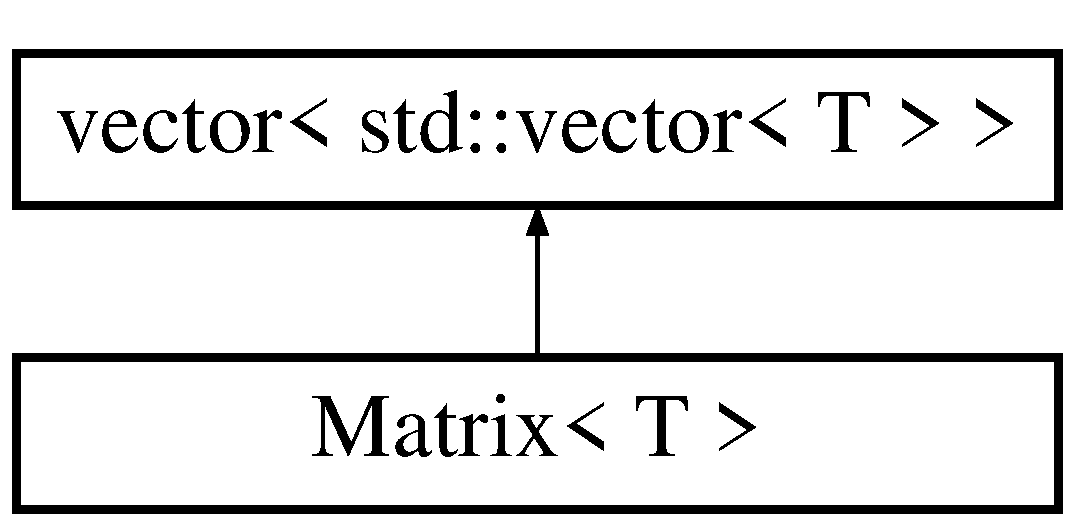
\includegraphics[height=2cm]{classMatrix}
\end{center}
\end{figure}
\subsection*{Public Methods}
\begin{CompactItemize}
\item 
{\bf Matrix} ()
\item 
{\bf Matrix} (const int \&)
\item 
{\bf Matrix} (const int \&, const int \&)
\item 
{\bf std::vector}$<$ T $>$ {\bf operator $\ast$} (const {\bf std::vector}$<$ T $>$ \&) const
\item 
{\bf std::vector}$<$ T $>$ {\bf get\-Column} (const int) const
\item 
Matrix$<$ T $>$ {\bf operator $\ast$} (const Matrix$<$ T $>$ \&) const
\item 
void {\bf print} ()
\end{CompactItemize}
\subsubsection*{template$<$class T$>$ class Matrix$<$ T $>$}



\subsection{Constructor \& Destructor Documentation}
\index{Matrix@{Matrix}!Matrix@{Matrix}}
\index{Matrix@{Matrix}!Matrix@{Matrix}}
\subsubsection{\setlength{\rightskip}{0pt plus 5cm}template$<$class T$>$ Matrix$<$ T $>$::Matrix ()}\label{classMatrix_a0}


\index{Matrix@{Matrix}!Matrix@{Matrix}}
\index{Matrix@{Matrix}!Matrix@{Matrix}}
\subsubsection{\setlength{\rightskip}{0pt plus 5cm}template$<$class T$>$ Matrix$<$ T $>$::Matrix (const int \&)}\label{classMatrix_a1}


\index{Matrix@{Matrix}!Matrix@{Matrix}}
\index{Matrix@{Matrix}!Matrix@{Matrix}}
\subsubsection{\setlength{\rightskip}{0pt plus 5cm}template$<$class T$>$ Matrix$<$ T $>$::Matrix (const int \&, const int \&)}\label{classMatrix_a2}




\subsection{Member Function Documentation}
\index{Matrix@{Matrix}!getColumn@{getColumn}}
\index{getColumn@{getColumn}!Matrix@{Matrix}}
\subsubsection{\setlength{\rightskip}{0pt plus 5cm}template$<$class T$>$ {\bf std::vector}$<$ T $>$ Matrix$<$ T $>$::get\-Column (const {\em int}) const}\label{classMatrix_a4}


\index{Matrix@{Matrix}!operator *@{operator $\ast$}}
\index{operator *@{operator $\ast$}!Matrix@{Matrix}}
\subsubsection{\setlength{\rightskip}{0pt plus 5cm}template$<$class T$>$ Matrix$<$ T $>$ Matrix$<$ T $>$::operator $\ast$ (const Matrix$<$ T $>$ \&) const}\label{classMatrix_a5}


\index{Matrix@{Matrix}!operator *@{operator $\ast$}}
\index{operator *@{operator $\ast$}!Matrix@{Matrix}}
\subsubsection{\setlength{\rightskip}{0pt plus 5cm}template$<$class T$>$ {\bf std::vector}$<$ T $>$ Matrix$<$ T $>$::operator $\ast$ (const {\bf std::vector}$<$ T $>$ \&) const}\label{classMatrix_a3}


\index{Matrix@{Matrix}!print@{print}}
\index{print@{print}!Matrix@{Matrix}}
\subsubsection{\setlength{\rightskip}{0pt plus 5cm}template$<$class T$>$ void Matrix$<$ T $>$::print ()}\label{classMatrix_a6}




The documentation for this class was generated from the following file:\begin{CompactItemize}
\item 
{\bf matrix.h}\end{CompactItemize}

\section{Object Class Reference}
\label{classObject}\index{Object@{Object}}
{\tt \#include $<$object.h$>$}

Inheritance diagram for Object::\begin{figure}[H]
\begin{center}
\leavevmode
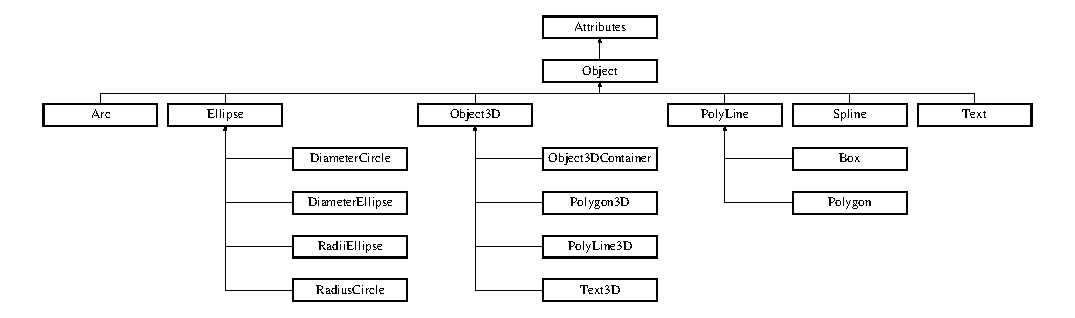
\includegraphics[height=3.82812cm]{classObject}
\end{center}
\end{figure}
\subsection*{Public Types}
\begin{CompactItemize}
\item 
enum {\bf Object\-Codes} \{ {\bf Pseudo\-Color\-Code} =  0, 
{\bf Arc\-Code} =  5, 
{\bf Compound\-Code} =  6, 
{\bf Ellipse\-Code} =  1, 
{\bf Poly\-Line\-Code} =  2, 
{\bf Spline\-Code} =  3, 
{\bf Text\-Code} =  4
 \}
\end{CompactItemize}
\subsection*{Public Methods}
\begin{CompactItemize}
\item 
{\bf Object} ()
\item 
virtual {\bf $\sim$Object} ()
\item 
{\bf Object\-Codes} {\bf get\-Code} ()
\item 
virtual void {\bf write} (std::ostream \&stream) const
\end{CompactItemize}
\subsection*{Protected Methods}
\begin{CompactItemize}
\item 
void {\bf set\-Code} ({\bf Object\-Codes} {\bf code})
\end{CompactItemize}
\subsection*{Protected Attributes}
\begin{CompactItemize}
\item 
{\bf Object\-Codes} {\bf code}
\end{CompactItemize}


\subsection{Detailed Description}
This generic class handles objects. This class is derived from {\bf Attributes} {\rm (p.\,\pageref{classAttributes})}. \begin{Desc}
\item[Author: ]\par
Anthony Liekens \end{Desc}




\subsection{Member Enumeration Documentation}
\index{Object@{Object}!ObjectCodes@{ObjectCodes}}
\index{ObjectCodes@{ObjectCodes}!Object@{Object}}
\subsubsection{\setlength{\rightskip}{0pt plus 5cm}enum Object::Object\-Codes}\label{classObject_s7}


Enumeration of object codes. The following object codes can be used to set the code of an object : \{$\backslash$tt Pseudo\-Color, {\bf Arc} {\rm (p.\,\pageref{classArc})}, Compound, Ellips, {\bf Poly\-Line} {\rm (p.\,\pageref{classPolyLine})}, {\bf Spline} {\rm (p.\,\pageref{classSpline})}, {\bf Text} {\rm (p.\,\pageref{classText})}\} \begin{Desc}
\item[Enumeration values: ]\par
\begin{description}
\index{PseudoColorCode@{PseudoColorCode}!Object@{Object}}\index{Object@{Object}!PseudoColorCode@{PseudoColorCode}}\item[{\em 
{\em Pseudo\-Color\-Code}\label{classObject_s7s0}
}]\index{ArcCode@{ArcCode}!Object@{Object}}\index{Object@{Object}!ArcCode@{ArcCode}}\item[{\em 
{\em Arc\-Code}\label{classObject_s7s1}
}]\index{CompoundCode@{CompoundCode}!Object@{Object}}\index{Object@{Object}!CompoundCode@{CompoundCode}}\item[{\em 
{\em Compound\-Code}\label{classObject_s7s2}
}]\index{EllipseCode@{EllipseCode}!Object@{Object}}\index{Object@{Object}!EllipseCode@{EllipseCode}}\item[{\em 
{\em Ellipse\-Code}\label{classObject_s7s3}
}]\index{PolyLineCode@{PolyLineCode}!Object@{Object}}\index{Object@{Object}!PolyLineCode@{PolyLineCode}}\item[{\em 
{\em Poly\-Line\-Code}\label{classObject_s7s4}
}]\index{SplineCode@{SplineCode}!Object@{Object}}\index{Object@{Object}!SplineCode@{SplineCode}}\item[{\em 
{\em Spline\-Code}\label{classObject_s7s5}
}]\index{TextCode@{TextCode}!Object@{Object}}\index{Object@{Object}!TextCode@{TextCode}}\item[{\em 
{\em Text\-Code}\label{classObject_s7s6}
}]\end{description}
\end{Desc}



\subsection{Constructor \& Destructor Documentation}
\index{Object@{Object}!Object@{Object}}
\index{Object@{Object}!Object@{Object}}
\subsubsection{\setlength{\rightskip}{0pt plus 5cm}Object::Object ()}\label{classObject_a0}


Constructor. This constructor does nothing special, since this is a generic and abstract class \index{Object@{Object}!~Object@{$\sim$Object}}
\index{~Object@{$\sim$Object}!Object@{Object}}
\subsubsection{\setlength{\rightskip}{0pt plus 5cm}Object::$\sim$Object ()\hspace{0.3cm}{\tt  [virtual]}}\label{classObject_a1}


Destructor. 

\subsection{Member Function Documentation}
\index{Object@{Object}!getCode@{getCode}}
\index{getCode@{getCode}!Object@{Object}}
\subsubsection{\setlength{\rightskip}{0pt plus 5cm}{\bf Object\-Codes} Object::get\-Code ()\hspace{0.3cm}{\tt  [inline]}}\label{classObject_a2}


Returns the code of an object \index{Object@{Object}!setCode@{setCode}}
\index{setCode@{setCode}!Object@{Object}}
\subsubsection{\setlength{\rightskip}{0pt plus 5cm}void Object::set\-Code ({\bf Object\-Codes} {\em code})\hspace{0.3cm}{\tt  [inline, protected]}}\label{classObject_b0}


Sets the code of an object. This method can only be called by instances of Object \begin{Desc}
\item[Parameters: ]\par
\begin{description}
\item[{\em 
code}]integer value \end{description}
\end{Desc}
\begin{Desc}
\item[Returns: ]\par
void \end{Desc}
\index{Object@{Object}!write@{write}}
\index{write@{write}!Object@{Object}}
\subsubsection{\setlength{\rightskip}{0pt plus 5cm}virtual void Object::write (std::ostream \& {\em stream}) const\hspace{0.3cm}{\tt  [inline, virtual]}}\label{classObject_a3}


Write the object to a given outstream. All inherited classes of object should provide this method, since it's called by {\bf Figure} {\rm (p.\,\pageref{classFigure})} (the object container) to output objects to a given stream. \begin{Desc}
\item[Parameters: ]\par
\begin{description}
\item[{\em 
stream}]output stream \end{description}
\end{Desc}
\begin{Desc}
\item[Returns: ]\par
void \end{Desc}


Reimplemented in {\bf Arc} {\rm (p.\,\pageref{classArc_a6})}, {\bf Ellipse} {\rm (p.\,\pageref{classEllipse_a13})}, {\bf Polygon3D} {\rm (p.\,\pageref{classPolygon3D_a8})}, {\bf Poly\-Line} {\rm (p.\,\pageref{classPolyLine_a4})}, {\bf Poly\-Line3D} {\rm (p.\,\pageref{classPolyLine3D_a8})}, {\bf Spline} {\rm (p.\,\pageref{classSpline_a5})}, {\bf Text} {\rm (p.\,\pageref{classText_a5})}, and {\bf Text3D} {\rm (p.\,\pageref{classText3D_a9})}.

\subsection{Member Data Documentation}
\index{Object@{Object}!code@{code}}
\index{code@{code}!Object@{Object}}
\subsubsection{\setlength{\rightskip}{0pt plus 5cm}{\bf Object\-Codes} Object::code\hspace{0.3cm}{\tt  [protected]}}\label{classObject_n0}




The documentation for this class was generated from the following files:\begin{CompactItemize}
\item 
{\bf object.h}\item 
{\bf object.cpp}\end{CompactItemize}

\section{Object3D Class Reference}
\label{classObject3D}\index{Object3D@{Object3D}}
{\tt \#include $<$object3d.h$>$}

Inheritance diagram for Object3D::\begin{figure}[H]
\begin{center}
\leavevmode
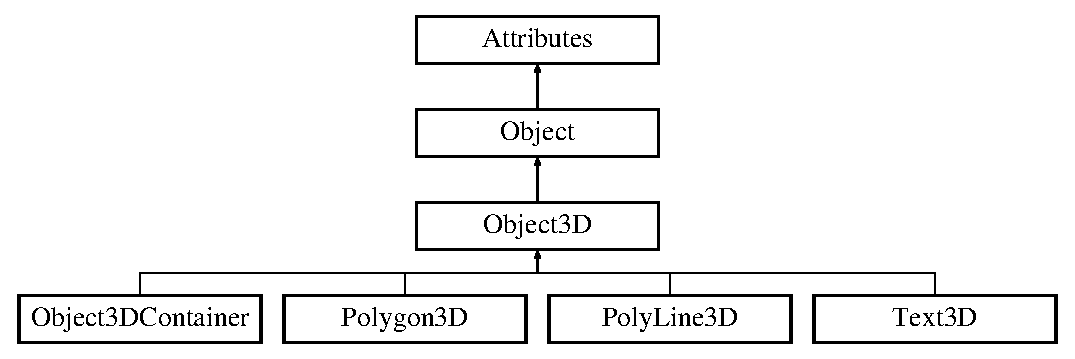
\includegraphics[height=4cm]{classObject3D}
\end{center}
\end{figure}
\subsection*{Public Methods}
\begin{CompactItemize}
\item 
virtual std::pair$<$ double, double $>$ {\bf get\-Depth\-Range} ()=0
\item 
virtual void {\bf render} ({\bf Figure} $\ast$, double x\-Offset, double y\-Offset, double scale, double distance, double min\-Depth, double max\-Depth, int min\-Fig\-Depth=0, int max\-Fig\-Depth=999)=0
\item 
virtual void {\bf apply\-Matrix} ({\bf Matrix}$<$ double $>$ $\ast$)=0
\item 
virtual void {\bf translate} ({\bf Coordinate3D} $\ast$)=0
\end{CompactItemize}


\subsection{Member Function Documentation}
\index{Object3D@{Object3D}!applyMatrix@{applyMatrix}}
\index{applyMatrix@{applyMatrix}!Object3D@{Object3D}}
\subsubsection{\setlength{\rightskip}{0pt plus 5cm}virtual void Object3D::apply\-Matrix ({\bf Matrix}$<$ double $>$ $\ast$)\hspace{0.3cm}{\tt  [pure virtual]}}\label{classObject3D_a2}




Implemented in {\bf Object3DContainer} {\rm (p.\,\pageref{classObject3DContainer_a2})}, {\bf Polygon3D} {\rm (p.\,\pageref{classPolygon3D_a6})}, {\bf Poly\-Line3D} {\rm (p.\,\pageref{classPolyLine3D_a5})}, and {\bf Text3D} {\rm (p.\,\pageref{classText3D_a7})}.\index{Object3D@{Object3D}!getDepthRange@{getDepthRange}}
\index{getDepthRange@{getDepthRange}!Object3D@{Object3D}}
\subsubsection{\setlength{\rightskip}{0pt plus 5cm}virtual std::pair$<$ double, double$>$ Object3D::get\-Depth\-Range ()\hspace{0.3cm}{\tt  [pure virtual]}}\label{classObject3D_a0}




Implemented in {\bf Object3DContainer} {\rm (p.\,\pageref{classObject3DContainer_a0})}, {\bf Polygon3D} {\rm (p.\,\pageref{classPolygon3D_a4})}, {\bf Poly\-Line3D} {\rm (p.\,\pageref{classPolyLine3D_a4})}, and {\bf Text3D} {\rm (p.\,\pageref{classText3D_a5})}.\index{Object3D@{Object3D}!render@{render}}
\index{render@{render}!Object3D@{Object3D}}
\subsubsection{\setlength{\rightskip}{0pt plus 5cm}virtual void Object3D::render ({\bf Figure} $\ast$, double {\em x\-Offset}, double {\em y\-Offset}, double {\em scale}, double {\em distance}, double {\em min\-Depth}, double {\em max\-Depth}, int {\em min\-Fig\-Depth} = 0, int {\em max\-Fig\-Depth} = 999)\hspace{0.3cm}{\tt  [pure virtual]}}\label{classObject3D_a1}




Implemented in {\bf Object3DContainer} {\rm (p.\,\pageref{classObject3DContainer_a1})}, {\bf Polygon3D} {\rm (p.\,\pageref{classPolygon3D_a5})}, {\bf Poly\-Line3D} {\rm (p.\,\pageref{classPolyLine3D_a6})}, and {\bf Text3D} {\rm (p.\,\pageref{classText3D_a6})}.\index{Object3D@{Object3D}!translate@{translate}}
\index{translate@{translate}!Object3D@{Object3D}}
\subsubsection{\setlength{\rightskip}{0pt plus 5cm}virtual void Object3D::translate ({\bf Coordinate3D} $\ast$)\hspace{0.3cm}{\tt  [pure virtual]}}\label{classObject3D_a3}




Implemented in {\bf Object3DContainer} {\rm (p.\,\pageref{classObject3DContainer_a3})}, {\bf Polygon3D} {\rm (p.\,\pageref{classPolygon3D_a7})}, {\bf Poly\-Line3D} {\rm (p.\,\pageref{classPolyLine3D_a7})}, and {\bf Text3D} {\rm (p.\,\pageref{classText3D_a8})}.

The documentation for this class was generated from the following file:\begin{CompactItemize}
\item 
{\bf object3d.h}\end{CompactItemize}

\section{Object3DContainer Class Reference}
\label{classObject3DContainer}\index{Object3DContainer@{Object3DContainer}}
{\tt \#include $<$object3dcontainer.h$>$}

Inheritance diagram for Object3DContainer::\begin{figure}[H]
\begin{center}
\leavevmode
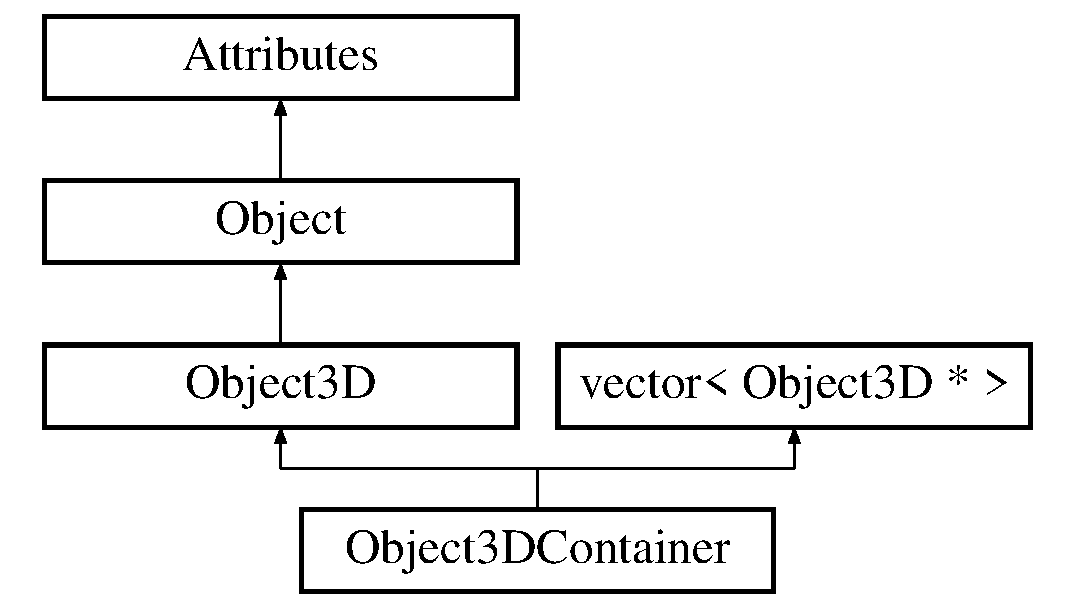
\includegraphics[height=4cm]{classObject3DContainer}
\end{center}
\end{figure}
\subsection*{Public Methods}
\begin{CompactItemize}
\item 
std::pair$<$ double, double $>$ {\bf get\-Depth\-Range} ()
\item 
void {\bf render} ({\bf Figure} $\ast$, double x\-Offset, double y\-Offset, double scale, double distance, double min\-Range=0, double max\-Range=0, int min\-Fig\-Depth=0, int max\-Fig\-Depth=999)
\item 
void {\bf apply\-Matrix} ({\bf Matrix}$<$ double $>$ $\ast$m)
\item 
void {\bf translate} ({\bf Coordinate3D} $\ast$)
\end{CompactItemize}


\subsection{Member Function Documentation}
\index{Object3DContainer@{Object3DContainer}!applyMatrix@{applyMatrix}}
\index{applyMatrix@{applyMatrix}!Object3DContainer@{Object3DContainer}}
\subsubsection{\setlength{\rightskip}{0pt plus 5cm}void Object3DContainer::apply\-Matrix ({\bf Matrix}$<$ double $>$ $\ast$ {\em m})\hspace{0.3cm}{\tt  [virtual]}}\label{classObject3DContainer_a2}




Implements {\bf Object3D} {\rm (p.\,\pageref{classObject3D_a2})}.\index{Object3DContainer@{Object3DContainer}!getDepthRange@{getDepthRange}}
\index{getDepthRange@{getDepthRange}!Object3DContainer@{Object3DContainer}}
\subsubsection{\setlength{\rightskip}{0pt plus 5cm}std::pair$<$ double, double $>$ Object3DContainer::get\-Depth\-Range ()\hspace{0.3cm}{\tt  [virtual]}}\label{classObject3DContainer_a0}




Implements {\bf Object3D} {\rm (p.\,\pageref{classObject3D_a0})}.\index{Object3DContainer@{Object3DContainer}!render@{render}}
\index{render@{render}!Object3DContainer@{Object3DContainer}}
\subsubsection{\setlength{\rightskip}{0pt plus 5cm}void Object3DContainer::render ({\bf Figure} $\ast$, double {\em x\-Offset}, double {\em y\-Offset}, double {\em scale}, double {\em distance}, double {\em min\-Range} = 0, double {\em max\-Range} = 0, int {\em min\-Fig\-Depth} = 0, int {\em max\-Fig\-Depth} = 999)\hspace{0.3cm}{\tt  [virtual]}}\label{classObject3DContainer_a1}




Implements {\bf Object3D} {\rm (p.\,\pageref{classObject3D_a1})}.\index{Object3DContainer@{Object3DContainer}!translate@{translate}}
\index{translate@{translate}!Object3DContainer@{Object3DContainer}}
\subsubsection{\setlength{\rightskip}{0pt plus 5cm}void Object3DContainer::translate ({\bf Coordinate3D} $\ast$)\hspace{0.3cm}{\tt  [virtual]}}\label{classObject3DContainer_a3}




Implements {\bf Object3D} {\rm (p.\,\pageref{classObject3D_a3})}.

The documentation for this class was generated from the following files:\begin{CompactItemize}
\item 
{\bf object3dcontainer.h}\item 
{\bf object3dcontainer.cpp}\end{CompactItemize}

\section{Polygon Class Reference}
\label{classPolygon}\index{Polygon@{Polygon}}
{\tt \#include $<$polygon.h$>$}

Inheritance diagram for Polygon::\begin{figure}[H]
\begin{center}
\leavevmode
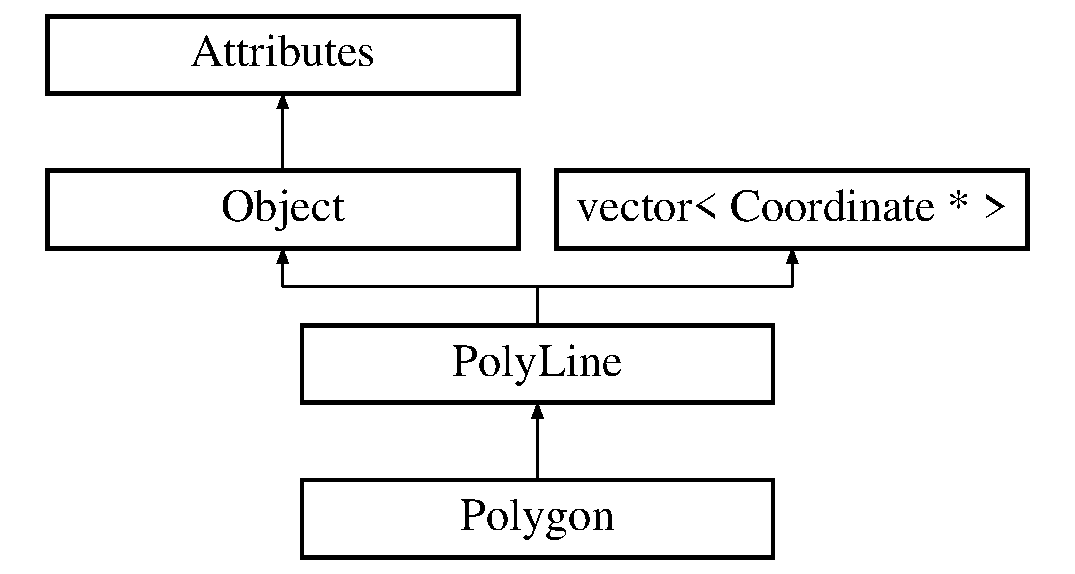
\includegraphics[height=4cm]{classPolygon}
\end{center}
\end{figure}
\subsection*{Public Methods}
\begin{CompactItemize}
\item 
{\bf Polygon} ()
\item 
{\bf Polygon} ({\bf Coordinate} $\ast$, {\bf Coordinate} $\ast$)
\item 
{\bf $\sim$Polygon} ()
\end{CompactItemize}


\subsection{Detailed Description}
This class handles polygons. This class is derived from {\bf Poly\-Line} {\rm (p.\,\pageref{classPolyLine})}. \begin{Desc}
\item[Author: ]\par
Anthony Liekens \end{Desc}




\subsection{Constructor \& Destructor Documentation}
\index{Polygon@{Polygon}!Polygon@{Polygon}}
\index{Polygon@{Polygon}!Polygon@{Polygon}}
\subsubsection{\setlength{\rightskip}{0pt plus 5cm}Polygon::Polygon ()}\label{classPolygon_a0}


\index{Polygon@{Polygon}!Polygon@{Polygon}}
\index{Polygon@{Polygon}!Polygon@{Polygon}}
\subsubsection{\setlength{\rightskip}{0pt plus 5cm}Polygon::Polygon ({\bf Coordinate} $\ast$, {\bf Coordinate} $\ast$)}\label{classPolygon_a1}


\index{Polygon@{Polygon}!~Polygon@{$\sim$Polygon}}
\index{~Polygon@{$\sim$Polygon}!Polygon@{Polygon}}
\subsubsection{\setlength{\rightskip}{0pt plus 5cm}Polygon::$\sim$Polygon ()}\label{classPolygon_a2}




The documentation for this class was generated from the following files:\begin{CompactItemize}
\item 
{\bf polygon.h}\item 
{\bf polygon.cpp}\end{CompactItemize}

\section{Polygon3D Class Reference}
\label{classPolygon3D}\index{Polygon3D@{Polygon3D}}
{\tt \#include $<$polygon3d.h$>$}

Inheritance diagram for Polygon3D::\begin{figure}[H]
\begin{center}
\leavevmode
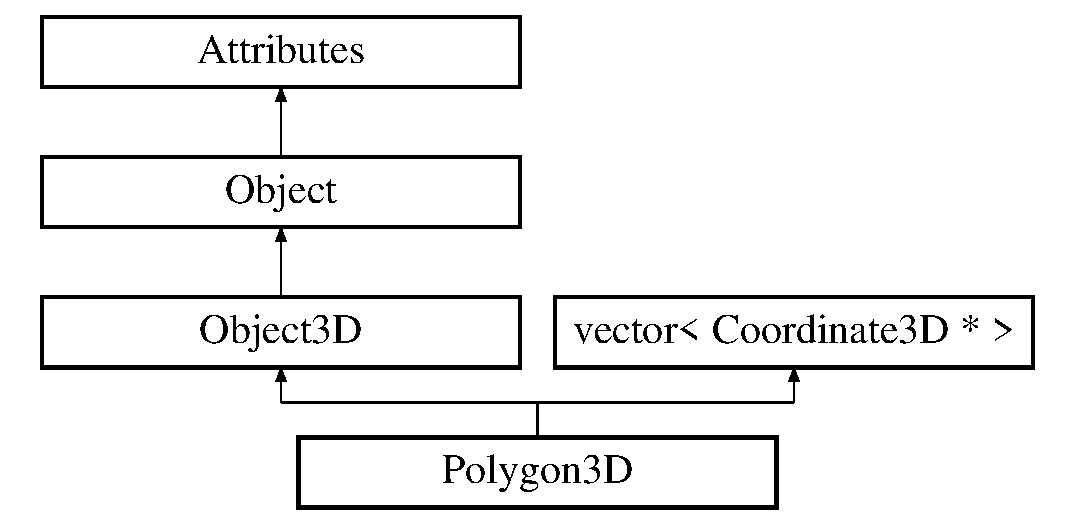
\includegraphics[height=4cm]{classPolygon3D}
\end{center}
\end{figure}
\subsection*{Public Types}
\begin{CompactItemize}
\item 
enum {\bf Sub\-Types} \{ {\bf Poly\-Line3DType} =   1, 
{\bf Box\-Type} =  2, 
{\bf Polygon\-Type} =  3, 
{\bf Arc\-Box\-Type} =  4, 
{\bf Picture\-Type} =  5
 \}
\end{CompactItemize}
\subsection*{Public Methods}
\begin{CompactItemize}
\item 
{\bf Polygon3D} ()
\item 
{\bf Polygon3D} ({\bf Coordinate3D} $\ast$point1, {\bf Coordinate3D} $\ast$point2)
\item 
{\bf $\sim$Polygon3D} ()
\item 
int {\bf get\-Sub\-Type} ()
\item 
std::pair$<$ double, double $>$ {\bf get\-Depth\-Range} ()
\item 
void {\bf render} ({\bf Figure} $\ast$, double x\-Offset, double y\-Offset, double scale, double distance, double min\-Depth, double max\-Depth, int min\-Fig\-Depth=0, int max\-Fig\-Depth=999)
\item 
void {\bf apply\-Matrix} ({\bf Matrix}$<$ double $>$ $\ast$)
\item 
void {\bf translate} ({\bf Coordinate3D} $\ast$)
\item 
void {\bf write} (std::ostream \&stream) const
\end{CompactItemize}
\subsection*{Protected Methods}
\begin{CompactItemize}
\item 
void {\bf set\-Sub\-Type} ({\bf Sub\-Types} {\bf sub\-Type})
\end{CompactItemize}
\subsection*{Private Attributes}
\begin{CompactItemize}
\item 
{\bf Sub\-Types} {\bf sub\-Type}
\end{CompactItemize}


\subsection{Member Enumeration Documentation}
\index{Polygon3D@{Polygon3D}!SubTypes@{SubTypes}}
\index{SubTypes@{SubTypes}!Polygon3D@{Polygon3D}}
\subsubsection{\setlength{\rightskip}{0pt plus 5cm}enum Polygon3D::Sub\-Types}\label{classPolygon3D_s5}


Enumeration of polygon types. The following types can be used to set the type of a polygon object : \{$\backslash$tt Polygon\-Type, Box\-Type, Polygon\-Type, Picture\-Type\}. Inherited polygon classes will set their appropriate type. \begin{Desc}
\item[Enumeration values: ]\par
\begin{description}
\index{PolyLine3DType@{PolyLine3DType}!Polygon3D@{Polygon3D}}\index{Polygon3D@{Polygon3D}!PolyLine3DType@{PolyLine3DType}}\item[{\em 
{\em Poly\-Line3DType}\label{classPolygon3D_s5s0}
}]\index{BoxType@{BoxType}!Polygon3D@{Polygon3D}}\index{Polygon3D@{Polygon3D}!BoxType@{BoxType}}\item[{\em 
{\em Box\-Type}\label{classPolygon3D_s5s1}
}]\index{PolygonType@{PolygonType}!Polygon3D@{Polygon3D}}\index{Polygon3D@{Polygon3D}!PolygonType@{PolygonType}}\item[{\em 
{\em Polygon\-Type}\label{classPolygon3D_s5s2}
}]\index{ArcBoxType@{ArcBoxType}!Polygon3D@{Polygon3D}}\index{Polygon3D@{Polygon3D}!ArcBoxType@{ArcBoxType}}\item[{\em 
{\em Arc\-Box\-Type}\label{classPolygon3D_s5s3}
}]\index{PictureType@{PictureType}!Polygon3D@{Polygon3D}}\index{Polygon3D@{Polygon3D}!PictureType@{PictureType}}\item[{\em 
{\em Picture\-Type}\label{classPolygon3D_s5s4}
}]\end{description}
\end{Desc}



\subsection{Constructor \& Destructor Documentation}
\index{Polygon3D@{Polygon3D}!Polygon3D@{Polygon3D}}
\index{Polygon3D@{Polygon3D}!Polygon3D@{Polygon3D}}
\subsubsection{\setlength{\rightskip}{0pt plus 5cm}Polygon3D::Polygon3D ()}\label{classPolygon3D_a0}


Constructor. Constructs a polygon object \index{Polygon3D@{Polygon3D}!Polygon3D@{Polygon3D}}
\index{Polygon3D@{Polygon3D}!Polygon3D@{Polygon3D}}
\subsubsection{\setlength{\rightskip}{0pt plus 5cm}Polygon3D::Polygon3D ({\bf Coordinate3D} $\ast$ {\em point1}, {\bf Coordinate3D} $\ast$ {\em point2})}\label{classPolygon3D_a1}


Constructor. Constructs a polygon object with 2 points \begin{Desc}
\item[Parameters: ]\par
\begin{description}
\item[{\em 
point1}]- Instance of {\bf Coordinate3D} {\rm (p.\,\pageref{classCoordinate3D})}. {\bf Coordinate3D} {\rm (p.\,\pageref{classCoordinate3D})} of the first point \item[{\em 
point2}]- Instance of {\bf Coordinate3D} {\rm (p.\,\pageref{classCoordinate3D})}. {\bf Coordinate3D} {\rm (p.\,\pageref{classCoordinate3D})} of the second point \end{description}
\end{Desc}
\index{Polygon3D@{Polygon3D}!~Polygon3D@{$\sim$Polygon3D}}
\index{~Polygon3D@{$\sim$Polygon3D}!Polygon3D@{Polygon3D}}
\subsubsection{\setlength{\rightskip}{0pt plus 5cm}Polygon3D::$\sim$Polygon3D ()}\label{classPolygon3D_a2}


Destructor. Destructs a polygon object 

\subsection{Member Function Documentation}
\index{Polygon3D@{Polygon3D}!applyMatrix@{applyMatrix}}
\index{applyMatrix@{applyMatrix}!Polygon3D@{Polygon3D}}
\subsubsection{\setlength{\rightskip}{0pt plus 5cm}void Polygon3D::apply\-Matrix ({\bf Matrix}$<$ double $>$ $\ast$)\hspace{0.3cm}{\tt  [virtual]}}\label{classPolygon3D_a6}




Implements {\bf Object3D} {\rm (p.\,\pageref{classObject3D_a2})}.\index{Polygon3D@{Polygon3D}!getDepthRange@{getDepthRange}}
\index{getDepthRange@{getDepthRange}!Polygon3D@{Polygon3D}}
\subsubsection{\setlength{\rightskip}{0pt plus 5cm}std::pair$<$ double, double $>$ Polygon3D::get\-Depth\-Range ()\hspace{0.3cm}{\tt  [virtual]}}\label{classPolygon3D_a4}




Implements {\bf Object3D} {\rm (p.\,\pageref{classObject3D_a0})}.\index{Polygon3D@{Polygon3D}!getSubType@{getSubType}}
\index{getSubType@{getSubType}!Polygon3D@{Polygon3D}}
\subsubsection{\setlength{\rightskip}{0pt plus 5cm}int Polygon3D::get\-Sub\-Type ()\hspace{0.3cm}{\tt  [inline]}}\label{classPolygon3D_a3}


Returns the polygon sub type \begin{Desc}
\item[Returns: ]\par
Instance of {\bf Sub\-Types} {\rm (p.\,\pageref{classPolygon3D_s5})} \end{Desc}
\index{Polygon3D@{Polygon3D}!render@{render}}
\index{render@{render}!Polygon3D@{Polygon3D}}
\subsubsection{\setlength{\rightskip}{0pt plus 5cm}void Polygon3D::render ({\bf Figure} $\ast$, double {\em x\-Offset}, double {\em y\-Offset}, double {\em scale}, double {\em distance}, double {\em min\-Depth}, double {\em max\-Depth}, int {\em min\-Fig\-Depth} = 0, int {\em max\-Fig\-Depth} = 999)\hspace{0.3cm}{\tt  [virtual]}}\label{classPolygon3D_a5}




Implements {\bf Object3D} {\rm (p.\,\pageref{classObject3D_a1})}.\index{Polygon3D@{Polygon3D}!setSubType@{setSubType}}
\index{setSubType@{setSubType}!Polygon3D@{Polygon3D}}
\subsubsection{\setlength{\rightskip}{0pt plus 5cm}void Polygon3D::set\-Sub\-Type ({\bf Sub\-Types} {\em sub\-Type})\hspace{0.3cm}{\tt  [inline, protected]}}\label{classPolygon3D_b0}


Set the sub type \begin{Desc}
\item[Parameters: ]\par
\begin{description}
\item[{\em 
sub\-Type}]{\bf Sub\-Types} {\rm (p.\,\pageref{classPolygon3D_s5})} \end{description}
\end{Desc}
\begin{Desc}
\item[Returns: ]\par
void \end{Desc}
\index{Polygon3D@{Polygon3D}!translate@{translate}}
\index{translate@{translate}!Polygon3D@{Polygon3D}}
\subsubsection{\setlength{\rightskip}{0pt plus 5cm}void Polygon3D::translate ({\bf Coordinate3D} $\ast$)\hspace{0.3cm}{\tt  [virtual]}}\label{classPolygon3D_a7}




Implements {\bf Object3D} {\rm (p.\,\pageref{classObject3D_a3})}.\index{Polygon3D@{Polygon3D}!write@{write}}
\index{write@{write}!Polygon3D@{Polygon3D}}
\subsubsection{\setlength{\rightskip}{0pt plus 5cm}void Polygon3D::write (std::ostream \& {\em stream}) const\hspace{0.3cm}{\tt  [virtual]}}\label{classPolygon3D_a8}


Write the polygon object to a given outstream. \begin{Desc}
\item[Parameters: ]\par
\begin{description}
\item[{\em 
stream}]output stream \end{description}
\end{Desc}
\begin{Desc}
\item[Returns: ]\par
void \end{Desc}


Reimplemented from {\bf Object} {\rm (p.\,\pageref{classObject_a3})}.

\subsection{Member Data Documentation}
\index{Polygon3D@{Polygon3D}!subType@{subType}}
\index{subType@{subType}!Polygon3D@{Polygon3D}}
\subsubsection{\setlength{\rightskip}{0pt plus 5cm}{\bf Sub\-Types} Polygon3D::sub\-Type\hspace{0.3cm}{\tt  [private]}}\label{classPolygon3D_o0}




The documentation for this class was generated from the following files:\begin{CompactItemize}
\item 
{\bf polygon3d.h}\item 
{\bf polygon3d.cpp}\end{CompactItemize}

\section{Poly\-Line Class Reference}
\label{classPolyLine}\index{PolyLine@{PolyLine}}
{\tt \#include $<$polyline.h$>$}

Inheritance diagram for Poly\-Line::\begin{figure}[H]
\begin{center}
\leavevmode
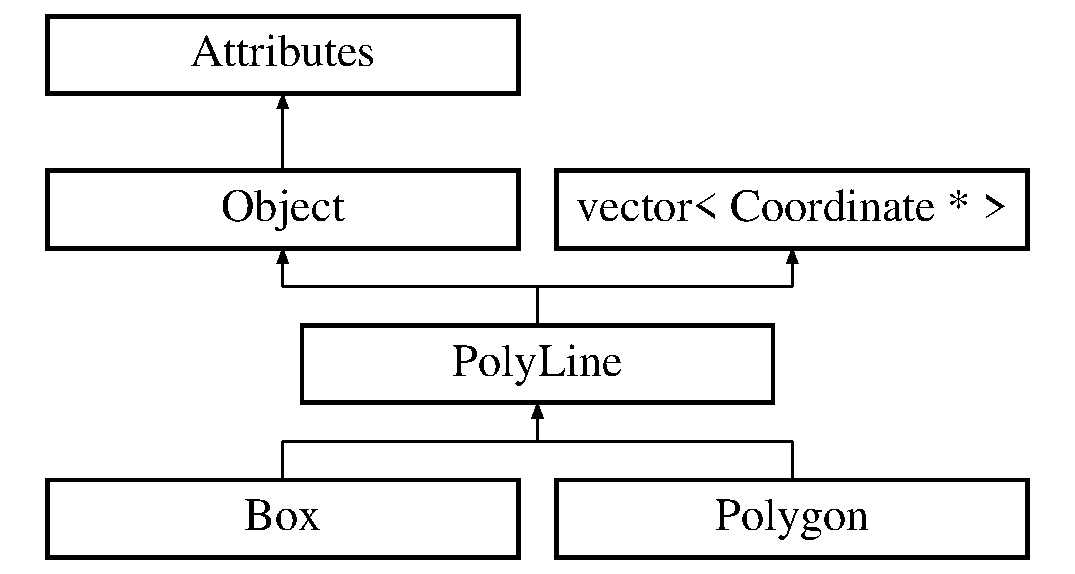
\includegraphics[height=4cm]{classPolyLine}
\end{center}
\end{figure}
\subsection*{Public Types}
\begin{CompactItemize}
\item 
enum {\bf Sub\-Types} \{ {\bf Poly\-Line\-Type} =   1, 
{\bf Box\-Type} =  2, 
{\bf Polygon\-Type} =  3, 
{\bf Arc\-Box\-Type} =  4, 
{\bf Picture\-Type} =  5
 \}
\end{CompactItemize}
\subsection*{Public Methods}
\begin{CompactItemize}
\item 
{\bf Poly\-Line} ()
\item 
{\bf Poly\-Line} ({\bf Coordinate} $\ast$point1, {\bf Coordinate} $\ast$point2)
\item 
{\bf $\sim$Poly\-Line} ()
\item 
int {\bf get\-Sub\-Type} ()
\item 
void {\bf write} (std::ostream \&stream) const
\end{CompactItemize}
\subsection*{Protected Methods}
\begin{CompactItemize}
\item 
void {\bf set\-Sub\-Type} ({\bf Sub\-Types} {\bf sub\-Type})
\end{CompactItemize}
\subsection*{Private Attributes}
\begin{CompactItemize}
\item 
{\bf Sub\-Types} {\bf sub\-Type}
\end{CompactItemize}


\subsection{Detailed Description}
This class handles polyline objects. This class is derived from {\bf Object} {\rm (p.\,\pageref{classObject})}. It acts as a vector (C++ standard library) container for instances of {\bf Coordinate} {\rm (p.\,\pageref{classCoordinate})} \begin{Desc}
\item[Author: ]\par
Anthony Liekens \end{Desc}




\subsection{Member Enumeration Documentation}
\index{PolyLine@{Poly\-Line}!SubTypes@{SubTypes}}
\index{SubTypes@{SubTypes}!PolyLine@{Poly\-Line}}
\subsubsection{\setlength{\rightskip}{0pt plus 5cm}enum Poly\-Line::Sub\-Types}\label{classPolyLine_s5}


Enumeration of polyline types. The following types can be used to set the type of a polyline object : \{$\backslash$tt Poly\-Line\-Type, Box\-Type, Polygon\-Type, Picture\-Type\}. Inherited polyline classes will set their appropriate type. \begin{Desc}
\item[Enumeration values: ]\par
\begin{description}
\index{PolyLineType@{PolyLineType}!PolyLine@{PolyLine}}\index{PolyLine@{PolyLine}!PolyLineType@{PolyLineType}}\item[{\em 
{\em Poly\-Line\-Type}\label{classPolyLine_s5s0}
}]\index{BoxType@{BoxType}!PolyLine@{PolyLine}}\index{PolyLine@{PolyLine}!BoxType@{BoxType}}\item[{\em 
{\em Box\-Type}\label{classPolyLine_s5s1}
}]\index{PolygonType@{PolygonType}!PolyLine@{PolyLine}}\index{PolyLine@{PolyLine}!PolygonType@{PolygonType}}\item[{\em 
{\em Polygon\-Type}\label{classPolyLine_s5s2}
}]\index{ArcBoxType@{ArcBoxType}!PolyLine@{PolyLine}}\index{PolyLine@{PolyLine}!ArcBoxType@{ArcBoxType}}\item[{\em 
{\em Arc\-Box\-Type}\label{classPolyLine_s5s3}
}]\index{PictureType@{PictureType}!PolyLine@{PolyLine}}\index{PolyLine@{PolyLine}!PictureType@{PictureType}}\item[{\em 
{\em Picture\-Type}\label{classPolyLine_s5s4}
}]\end{description}
\end{Desc}



\subsection{Constructor \& Destructor Documentation}
\index{PolyLine@{Poly\-Line}!PolyLine@{PolyLine}}
\index{PolyLine@{PolyLine}!PolyLine@{Poly\-Line}}
\subsubsection{\setlength{\rightskip}{0pt plus 5cm}Poly\-Line::Poly\-Line ()}\label{classPolyLine_a0}


Constructor. Constructs a polyline object \index{PolyLine@{Poly\-Line}!PolyLine@{PolyLine}}
\index{PolyLine@{PolyLine}!PolyLine@{Poly\-Line}}
\subsubsection{\setlength{\rightskip}{0pt plus 5cm}Poly\-Line::Poly\-Line ({\bf Coordinate} $\ast$ {\em point1}, {\bf Coordinate} $\ast$ {\em point2})}\label{classPolyLine_a1}


Constructor. Constructs a polyline object with 2 points \begin{Desc}
\item[Parameters: ]\par
\begin{description}
\item[{\em 
point1}]- Instance of {\bf Coordinate} {\rm (p.\,\pageref{classCoordinate})}. Coordinates of the first point \item[{\em 
point2}]- Instance of {\bf Coordinate} {\rm (p.\,\pageref{classCoordinate})}. Coordinates of the second point \end{description}
\end{Desc}
\index{PolyLine@{Poly\-Line}!~PolyLine@{$\sim$PolyLine}}
\index{~PolyLine@{$\sim$PolyLine}!PolyLine@{Poly\-Line}}
\subsubsection{\setlength{\rightskip}{0pt plus 5cm}Poly\-Line::$\sim$Poly\-Line ()}\label{classPolyLine_a2}


Destructor. Destructs a polyline object 

\subsection{Member Function Documentation}
\index{PolyLine@{Poly\-Line}!getSubType@{getSubType}}
\index{getSubType@{getSubType}!PolyLine@{Poly\-Line}}
\subsubsection{\setlength{\rightskip}{0pt plus 5cm}int Poly\-Line::get\-Sub\-Type ()\hspace{0.3cm}{\tt  [inline]}}\label{classPolyLine_a3}


Returns the polyline sub type \begin{Desc}
\item[Returns: ]\par
Instance of {\bf Sub\-Types} {\rm (p.\,\pageref{classPolyLine_s5})} \end{Desc}
\index{PolyLine@{Poly\-Line}!setSubType@{setSubType}}
\index{setSubType@{setSubType}!PolyLine@{Poly\-Line}}
\subsubsection{\setlength{\rightskip}{0pt plus 5cm}void Poly\-Line::set\-Sub\-Type ({\bf Sub\-Types} {\em sub\-Type})\hspace{0.3cm}{\tt  [inline, protected]}}\label{classPolyLine_b0}


Set the sub type \begin{Desc}
\item[Parameters: ]\par
\begin{description}
\item[{\em 
sub\-Type}]{\bf Sub\-Types} {\rm (p.\,\pageref{classPolyLine_s5})} \end{description}
\end{Desc}
\begin{Desc}
\item[Returns: ]\par
void \end{Desc}
\index{PolyLine@{Poly\-Line}!write@{write}}
\index{write@{write}!PolyLine@{Poly\-Line}}
\subsubsection{\setlength{\rightskip}{0pt plus 5cm}void Poly\-Line::write (std::ostream \& {\em stream}) const\hspace{0.3cm}{\tt  [virtual]}}\label{classPolyLine_a4}


Write the polyline object to a given outstream. \begin{Desc}
\item[Parameters: ]\par
\begin{description}
\item[{\em 
stream}]output stream \end{description}
\end{Desc}
\begin{Desc}
\item[Returns: ]\par
void \end{Desc}


Reimplemented from {\bf Object} {\rm (p.\,\pageref{classObject_a3})}.

\subsection{Member Data Documentation}
\index{PolyLine@{Poly\-Line}!subType@{subType}}
\index{subType@{subType}!PolyLine@{Poly\-Line}}
\subsubsection{\setlength{\rightskip}{0pt plus 5cm}{\bf Sub\-Types} Poly\-Line::sub\-Type\hspace{0.3cm}{\tt  [private]}}\label{classPolyLine_o0}




The documentation for this class was generated from the following files:\begin{CompactItemize}
\item 
{\bf polyline.h}\item 
{\bf polyline.cpp}\end{CompactItemize}

\section{Poly\-Line3D Class Reference}
\label{classPolyLine3D}\index{PolyLine3D@{PolyLine3D}}
{\tt \#include $<$polyline3d.h$>$}

Inheritance diagram for Poly\-Line3D::\begin{figure}[H]
\begin{center}
\leavevmode
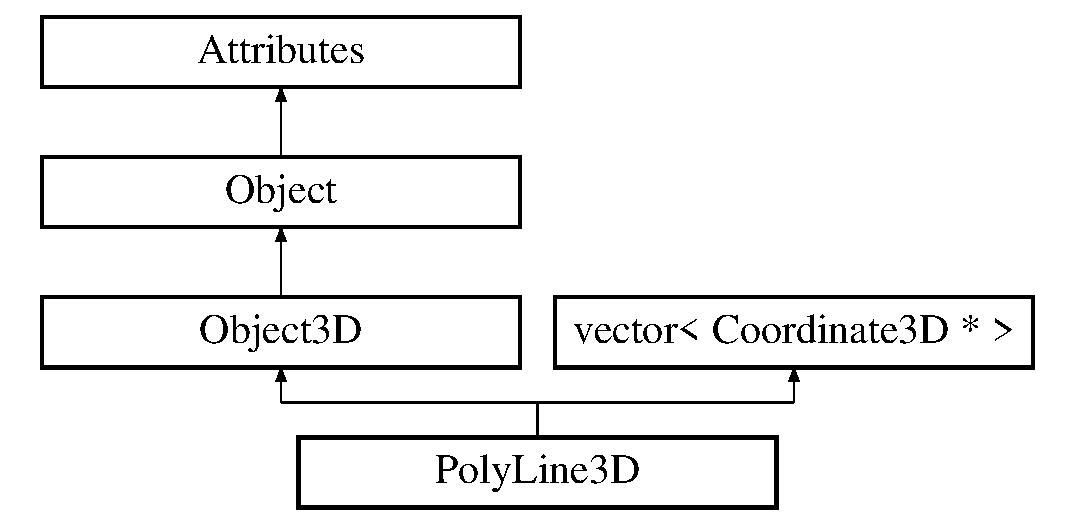
\includegraphics[height=4cm]{classPolyLine3D}
\end{center}
\end{figure}
\subsection*{Public Types}
\begin{CompactItemize}
\item 
enum {\bf Sub\-Types} \{ {\bf Poly\-Line3DType} =   1, 
{\bf Box\-Type} =  2, 
{\bf Polygon\-Type} =  3, 
{\bf Arc\-Box\-Type} =  4, 
{\bf Picture\-Type} =  5
 \}
\end{CompactItemize}
\subsection*{Public Methods}
\begin{CompactItemize}
\item 
{\bf Poly\-Line3D} ()
\item 
{\bf Poly\-Line3D} ({\bf Coordinate3D} $\ast$point1, {\bf Coordinate3D} $\ast$point2)
\item 
{\bf $\sim$Poly\-Line3D} ()
\item 
int {\bf get\-Sub\-Type} ()
\item 
std::pair$<$ double, double $>$ {\bf get\-Depth\-Range} ()
\item 
void {\bf apply\-Matrix} ({\bf Matrix}$<$ double $>$ $\ast$)
\item 
void {\bf render} ({\bf Figure} $\ast$, double x\-Offset, double y\-Offset, double scale, double distance, double min\-Depth, double max\-Depth, int min\-Fig\-Depth=0, int max\-Fig\-Depth=999)
\item 
void {\bf translate} ({\bf Coordinate3D} $\ast$)
\item 
void {\bf write} (std::ostream \&stream) const
\end{CompactItemize}
\subsection*{Protected Methods}
\begin{CompactItemize}
\item 
void {\bf set\-Sub\-Type} ({\bf Sub\-Types} {\bf sub\-Type})
\end{CompactItemize}
\subsection*{Private Attributes}
\begin{CompactItemize}
\item 
{\bf Sub\-Types} {\bf sub\-Type}
\end{CompactItemize}


\subsection{Member Enumeration Documentation}
\index{PolyLine3D@{Poly\-Line3D}!SubTypes@{SubTypes}}
\index{SubTypes@{SubTypes}!PolyLine3D@{Poly\-Line3D}}
\subsubsection{\setlength{\rightskip}{0pt plus 5cm}enum Poly\-Line3D::Sub\-Types}\label{classPolyLine3D_s5}


Enumeration of polyline types. The following types can be used to set the type of a polyline object : \{$\backslash$tt Poly\-Line\-Type, Box\-Type, Polygon\-Type, Picture\-Type\}. Inherited polyline classes will set their appropriate type. \begin{Desc}
\item[Enumeration values: ]\par
\begin{description}
\index{PolyLine3DType@{PolyLine3DType}!PolyLine3D@{PolyLine3D}}\index{PolyLine3D@{PolyLine3D}!PolyLine3DType@{PolyLine3DType}}\item[{\em 
{\em Poly\-Line3DType}\label{classPolyLine3D_s5s0}
}]\index{BoxType@{BoxType}!PolyLine3D@{PolyLine3D}}\index{PolyLine3D@{PolyLine3D}!BoxType@{BoxType}}\item[{\em 
{\em Box\-Type}\label{classPolyLine3D_s5s1}
}]\index{PolygonType@{PolygonType}!PolyLine3D@{PolyLine3D}}\index{PolyLine3D@{PolyLine3D}!PolygonType@{PolygonType}}\item[{\em 
{\em Polygon\-Type}\label{classPolyLine3D_s5s2}
}]\index{ArcBoxType@{ArcBoxType}!PolyLine3D@{PolyLine3D}}\index{PolyLine3D@{PolyLine3D}!ArcBoxType@{ArcBoxType}}\item[{\em 
{\em Arc\-Box\-Type}\label{classPolyLine3D_s5s3}
}]\index{PictureType@{PictureType}!PolyLine3D@{PolyLine3D}}\index{PolyLine3D@{PolyLine3D}!PictureType@{PictureType}}\item[{\em 
{\em Picture\-Type}\label{classPolyLine3D_s5s4}
}]\end{description}
\end{Desc}



\subsection{Constructor \& Destructor Documentation}
\index{PolyLine3D@{Poly\-Line3D}!PolyLine3D@{PolyLine3D}}
\index{PolyLine3D@{PolyLine3D}!PolyLine3D@{Poly\-Line3D}}
\subsubsection{\setlength{\rightskip}{0pt plus 5cm}Poly\-Line3D::Poly\-Line3D ()}\label{classPolyLine3D_a0}


Constructor. Constructs a polyline object \index{PolyLine3D@{Poly\-Line3D}!PolyLine3D@{PolyLine3D}}
\index{PolyLine3D@{PolyLine3D}!PolyLine3D@{Poly\-Line3D}}
\subsubsection{\setlength{\rightskip}{0pt plus 5cm}Poly\-Line3D::Poly\-Line3D ({\bf Coordinate3D} $\ast$ {\em point1}, {\bf Coordinate3D} $\ast$ {\em point2})}\label{classPolyLine3D_a1}


Constructor. Constructs a polyline object with 2 points \begin{Desc}
\item[Parameters: ]\par
\begin{description}
\item[{\em 
point1}]- Instance of {\bf Coordinate3D} {\rm (p.\,\pageref{classCoordinate3D})}. {\bf Coordinate3D} {\rm (p.\,\pageref{classCoordinate3D})} of the first point \item[{\em 
point2}]- Instance of {\bf Coordinate3D} {\rm (p.\,\pageref{classCoordinate3D})}. {\bf Coordinate3D} {\rm (p.\,\pageref{classCoordinate3D})} of the second point \end{description}
\end{Desc}
\index{PolyLine3D@{Poly\-Line3D}!~PolyLine3D@{$\sim$PolyLine3D}}
\index{~PolyLine3D@{$\sim$PolyLine3D}!PolyLine3D@{Poly\-Line3D}}
\subsubsection{\setlength{\rightskip}{0pt plus 5cm}Poly\-Line3D::$\sim$Poly\-Line3D ()}\label{classPolyLine3D_a2}


Destructor. Destructs a polyline object 

\subsection{Member Function Documentation}
\index{PolyLine3D@{Poly\-Line3D}!applyMatrix@{applyMatrix}}
\index{applyMatrix@{applyMatrix}!PolyLine3D@{Poly\-Line3D}}
\subsubsection{\setlength{\rightskip}{0pt plus 5cm}void Poly\-Line3D::apply\-Matrix ({\bf Matrix}$<$ double $>$ $\ast$)\hspace{0.3cm}{\tt  [virtual]}}\label{classPolyLine3D_a5}




Implements {\bf Object3D} {\rm (p.\,\pageref{classObject3D_a2})}.\index{PolyLine3D@{Poly\-Line3D}!getDepthRange@{getDepthRange}}
\index{getDepthRange@{getDepthRange}!PolyLine3D@{Poly\-Line3D}}
\subsubsection{\setlength{\rightskip}{0pt plus 5cm}std::pair$<$ double, double $>$ Poly\-Line3D::get\-Depth\-Range ()\hspace{0.3cm}{\tt  [virtual]}}\label{classPolyLine3D_a4}




Implements {\bf Object3D} {\rm (p.\,\pageref{classObject3D_a0})}.\index{PolyLine3D@{Poly\-Line3D}!getSubType@{getSubType}}
\index{getSubType@{getSubType}!PolyLine3D@{Poly\-Line3D}}
\subsubsection{\setlength{\rightskip}{0pt plus 5cm}int Poly\-Line3D::get\-Sub\-Type ()\hspace{0.3cm}{\tt  [inline]}}\label{classPolyLine3D_a3}


Returns the polyline sub type \begin{Desc}
\item[Returns: ]\par
Instance of {\bf Sub\-Types} {\rm (p.\,\pageref{classPolyLine3D_s5})} \end{Desc}
\index{PolyLine3D@{Poly\-Line3D}!render@{render}}
\index{render@{render}!PolyLine3D@{Poly\-Line3D}}
\subsubsection{\setlength{\rightskip}{0pt plus 5cm}void Poly\-Line3D::render ({\bf Figure} $\ast$, double {\em x\-Offset}, double {\em y\-Offset}, double {\em scale}, double {\em distance}, double {\em min\-Depth}, double {\em max\-Depth}, int {\em min\-Fig\-Depth} = 0, int {\em max\-Fig\-Depth} = 999)\hspace{0.3cm}{\tt  [virtual]}}\label{classPolyLine3D_a6}




Implements {\bf Object3D} {\rm (p.\,\pageref{classObject3D_a1})}.\index{PolyLine3D@{Poly\-Line3D}!setSubType@{setSubType}}
\index{setSubType@{setSubType}!PolyLine3D@{Poly\-Line3D}}
\subsubsection{\setlength{\rightskip}{0pt plus 5cm}void Poly\-Line3D::set\-Sub\-Type ({\bf Sub\-Types} {\em sub\-Type})\hspace{0.3cm}{\tt  [inline, protected]}}\label{classPolyLine3D_b0}


Set the sub type \begin{Desc}
\item[Parameters: ]\par
\begin{description}
\item[{\em 
sub\-Type}]{\bf Sub\-Types} {\rm (p.\,\pageref{classPolyLine3D_s5})} \end{description}
\end{Desc}
\begin{Desc}
\item[Returns: ]\par
void \end{Desc}
\index{PolyLine3D@{Poly\-Line3D}!translate@{translate}}
\index{translate@{translate}!PolyLine3D@{Poly\-Line3D}}
\subsubsection{\setlength{\rightskip}{0pt plus 5cm}void Poly\-Line3D::translate ({\bf Coordinate3D} $\ast$)\hspace{0.3cm}{\tt  [virtual]}}\label{classPolyLine3D_a7}




Implements {\bf Object3D} {\rm (p.\,\pageref{classObject3D_a3})}.\index{PolyLine3D@{Poly\-Line3D}!write@{write}}
\index{write@{write}!PolyLine3D@{Poly\-Line3D}}
\subsubsection{\setlength{\rightskip}{0pt plus 5cm}void Poly\-Line3D::write (std::ostream \& {\em stream}) const\hspace{0.3cm}{\tt  [virtual]}}\label{classPolyLine3D_a8}


Write the polyline object to a given outstream. \begin{Desc}
\item[Parameters: ]\par
\begin{description}
\item[{\em 
stream}]output stream \end{description}
\end{Desc}
\begin{Desc}
\item[Returns: ]\par
void \end{Desc}


Reimplemented from {\bf Object} {\rm (p.\,\pageref{classObject_a3})}.

\subsection{Member Data Documentation}
\index{PolyLine3D@{Poly\-Line3D}!subType@{subType}}
\index{subType@{subType}!PolyLine3D@{Poly\-Line3D}}
\subsubsection{\setlength{\rightskip}{0pt plus 5cm}{\bf Sub\-Types} Poly\-Line3D::sub\-Type\hspace{0.3cm}{\tt  [private]}}\label{classPolyLine3D_o0}




The documentation for this class was generated from the following files:\begin{CompactItemize}
\item 
{\bf polyline3d.h}\item 
{\bf polyline3d.cpp}\end{CompactItemize}

\section{Radii\-Ellipse Class Reference}
\label{classRadiiEllipse}\index{RadiiEllipse@{RadiiEllipse}}
{\tt \#include $<$radiiellipse.h$>$}

Inheritance diagram for Radii\-Ellipse::\begin{figure}[H]
\begin{center}
\leavevmode
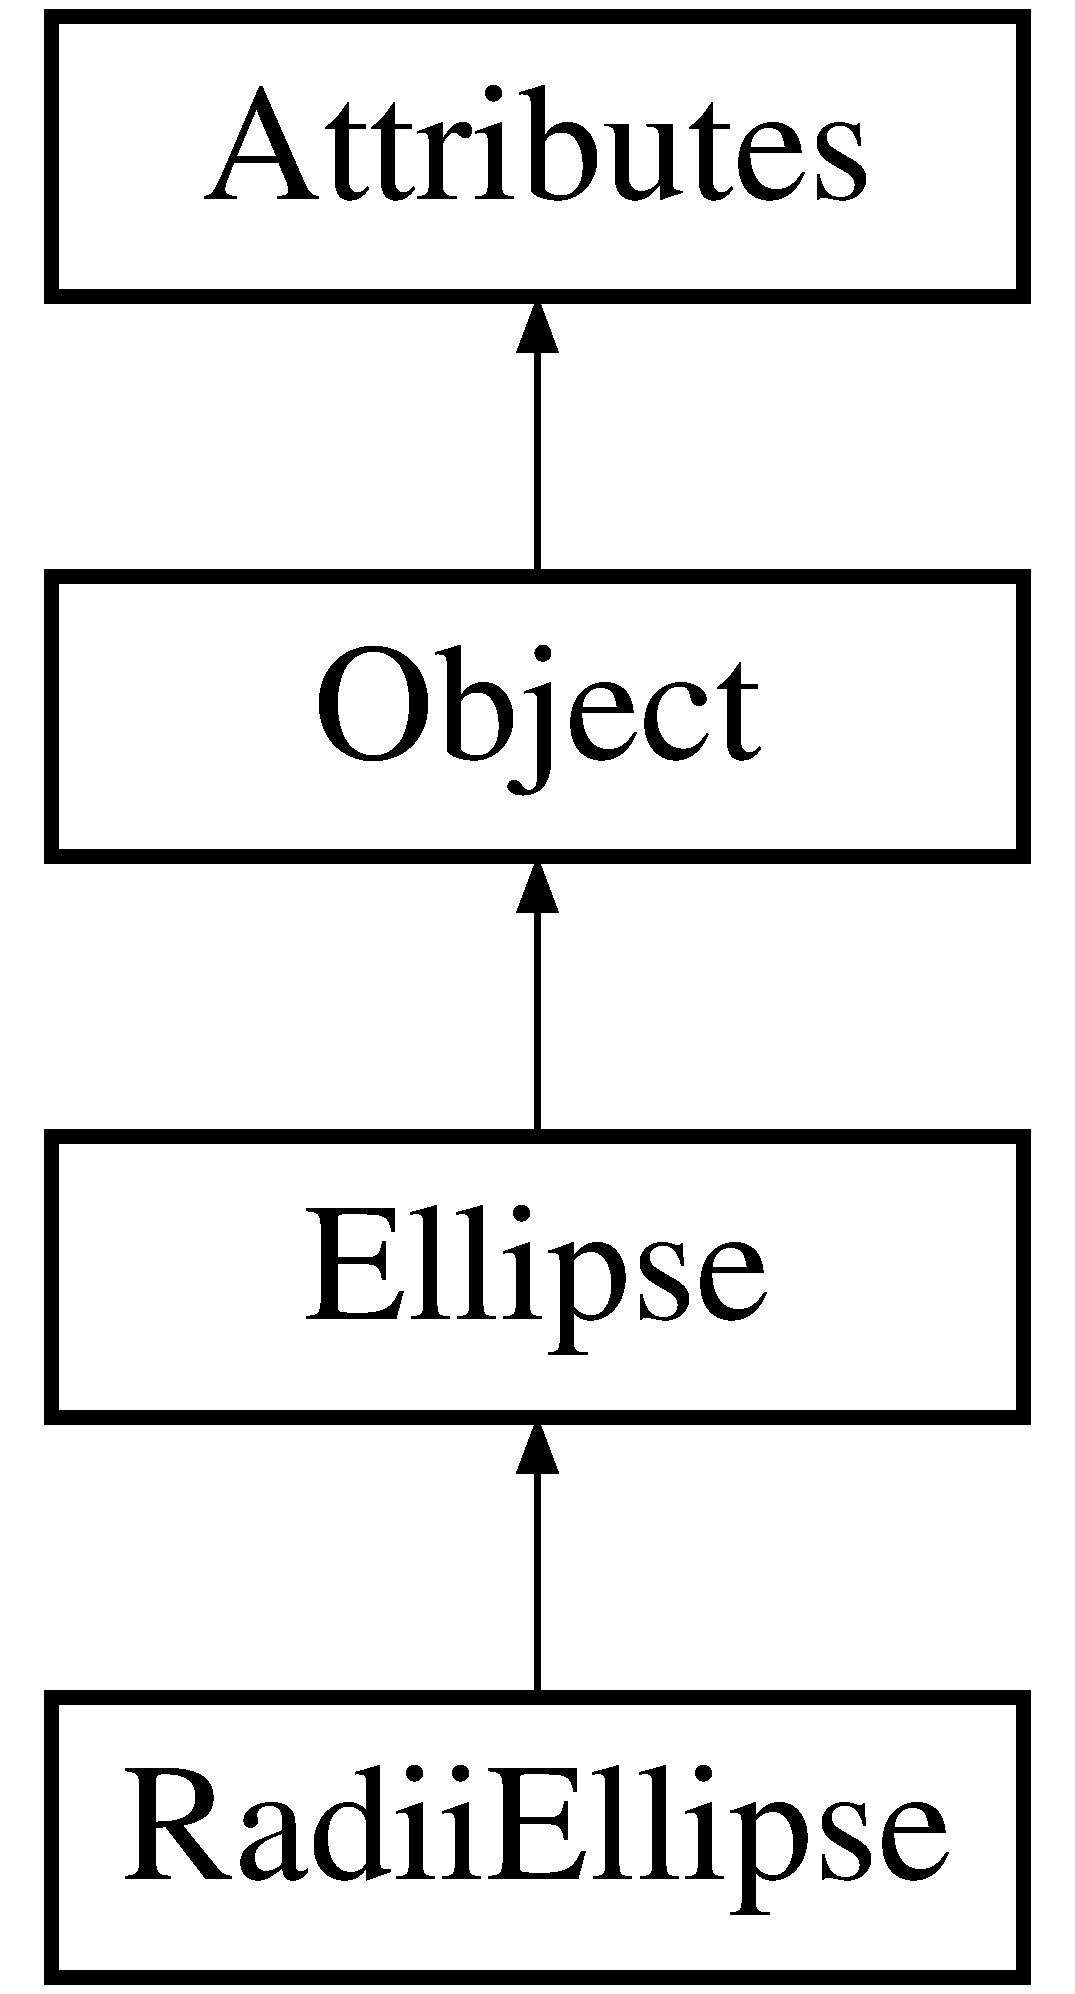
\includegraphics[height=4cm]{classRadiiEllipse}
\end{center}
\end{figure}
\subsection*{Public Methods}
\begin{CompactItemize}
\item 
{\bf Radii\-Ellipse} ()
\item 
{\bf Radii\-Ellipse} ({\bf Coordinate} $\ast$, {\bf Coordinate} $\ast$)
\item 
{\bf $\sim$Radii\-Ellipse} ()
\end{CompactItemize}


\subsection{Detailed Description}
This class handles ellipses defined by their center and radii. This class is derived from {\bf Ellipse} {\rm (p.\,\pageref{classEllipse})}. \begin{Desc}
\item[Author: ]\par
Anthony Liekens \end{Desc}




\subsection{Constructor \& Destructor Documentation}
\index{RadiiEllipse@{Radii\-Ellipse}!RadiiEllipse@{RadiiEllipse}}
\index{RadiiEllipse@{RadiiEllipse}!RadiiEllipse@{Radii\-Ellipse}}
\subsubsection{\setlength{\rightskip}{0pt plus 5cm}Radii\-Ellipse::Radii\-Ellipse ()}\label{classRadiiEllipse_a0}


\index{RadiiEllipse@{Radii\-Ellipse}!RadiiEllipse@{RadiiEllipse}}
\index{RadiiEllipse@{RadiiEllipse}!RadiiEllipse@{Radii\-Ellipse}}
\subsubsection{\setlength{\rightskip}{0pt plus 5cm}Radii\-Ellipse::Radii\-Ellipse ({\bf Coordinate} $\ast$, {\bf Coordinate} $\ast$)}\label{classRadiiEllipse_a1}


\index{RadiiEllipse@{Radii\-Ellipse}!~RadiiEllipse@{$\sim$RadiiEllipse}}
\index{~RadiiEllipse@{$\sim$RadiiEllipse}!RadiiEllipse@{Radii\-Ellipse}}
\subsubsection{\setlength{\rightskip}{0pt plus 5cm}Radii\-Ellipse::$\sim$Radii\-Ellipse ()}\label{classRadiiEllipse_a2}




The documentation for this class was generated from the following files:\begin{CompactItemize}
\item 
{\bf radiiellipse.h}\item 
{\bf radiiellipse.cpp}\end{CompactItemize}

\section{Radius\-Circle Class Reference}
\label{classRadiusCircle}\index{RadiusCircle@{RadiusCircle}}
{\tt \#include $<$radiuscircle.h$>$}

Inheritance diagram for Radius\-Circle::\begin{figure}[H]
\begin{center}
\leavevmode
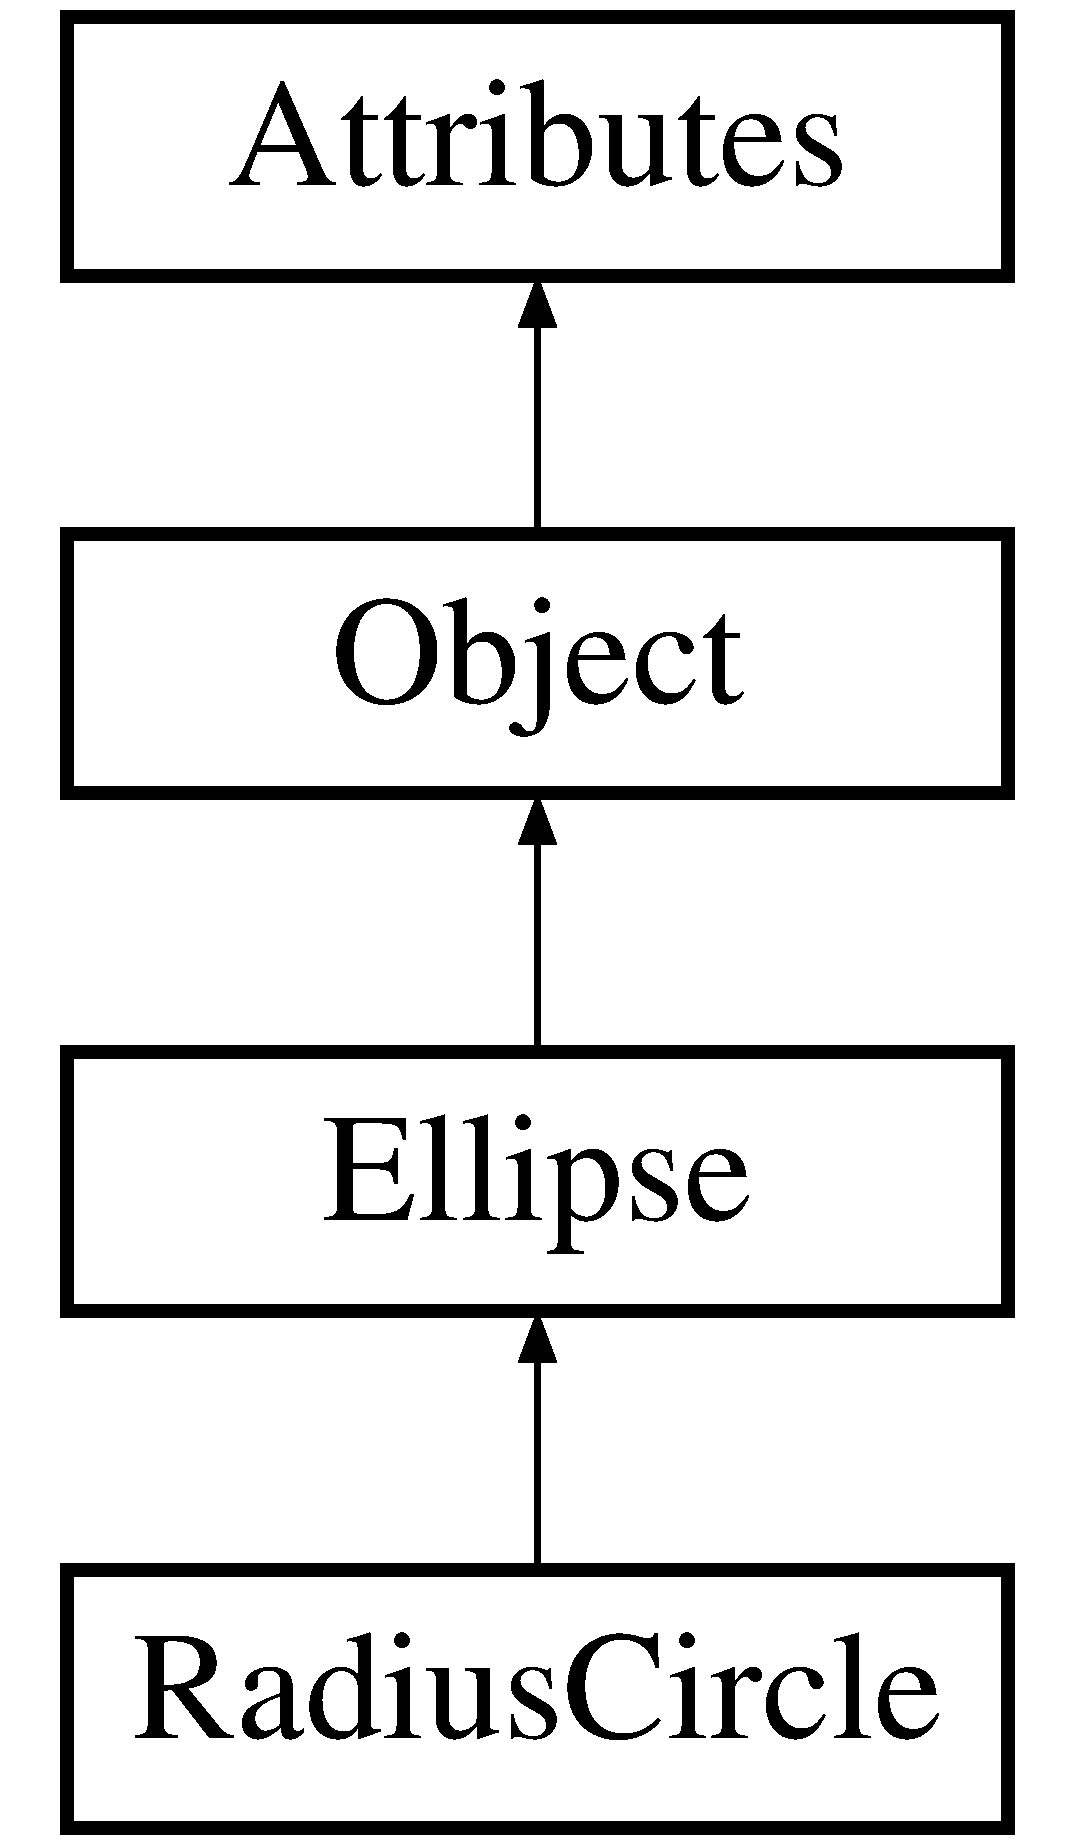
\includegraphics[height=4cm]{classRadiusCircle}
\end{center}
\end{figure}
\subsection*{Public Methods}
\begin{CompactItemize}
\item 
{\bf Radius\-Circle} ()
\item 
{\bf Radius\-Circle} ({\bf Coordinate} $\ast$, int)
\item 
{\bf $\sim$Radius\-Circle} ()
\end{CompactItemize}


\subsection{Detailed Description}
This class handles circles defined by their center and radius. This class is derived from {\bf Ellipse} {\rm (p.\,\pageref{classEllipse})}. \begin{Desc}
\item[Author: ]\par
Anthony Liekens \end{Desc}




\subsection{Constructor \& Destructor Documentation}
\index{RadiusCircle@{Radius\-Circle}!RadiusCircle@{RadiusCircle}}
\index{RadiusCircle@{RadiusCircle}!RadiusCircle@{Radius\-Circle}}
\subsubsection{\setlength{\rightskip}{0pt plus 5cm}Radius\-Circle::Radius\-Circle ()}\label{classRadiusCircle_a0}


\index{RadiusCircle@{Radius\-Circle}!RadiusCircle@{RadiusCircle}}
\index{RadiusCircle@{RadiusCircle}!RadiusCircle@{Radius\-Circle}}
\subsubsection{\setlength{\rightskip}{0pt plus 5cm}Radius\-Circle::Radius\-Circle ({\bf Coordinate} $\ast$, int)}\label{classRadiusCircle_a1}


\index{RadiusCircle@{Radius\-Circle}!~RadiusCircle@{$\sim$RadiusCircle}}
\index{~RadiusCircle@{$\sim$RadiusCircle}!RadiusCircle@{Radius\-Circle}}
\subsubsection{\setlength{\rightskip}{0pt plus 5cm}Radius\-Circle::$\sim$Radius\-Circle ()}\label{classRadiusCircle_a2}




The documentation for this class was generated from the following files:\begin{CompactItemize}
\item 
{\bf radiuscircle.h}\item 
{\bf radiuscircle.cpp}\end{CompactItemize}

\section{Rotation3DMatrix Class Reference}
\label{classRotation3DMatrix}\index{Rotation3DMatrix@{Rotation3DMatrix}}
{\tt \#include $<$rotation3dmatrix.h$>$}

Inheritance diagram for Rotation3DMatrix::\begin{figure}[H]
\begin{center}
\leavevmode
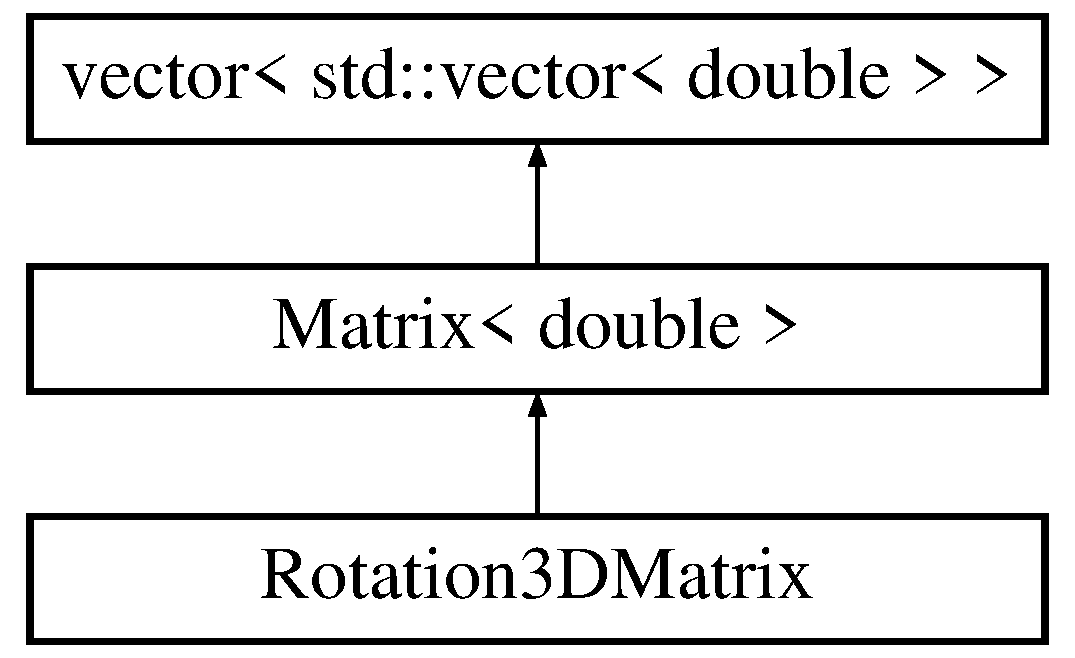
\includegraphics[height=3cm]{classRotation3DMatrix}
\end{center}
\end{figure}
\subsection*{Public Methods}
\begin{CompactItemize}
\item 
{\bf Rotation3DMatrix} (double x\-Corner, double y\-Corner, double z\-Corner)
\end{CompactItemize}


\subsection{Constructor \& Destructor Documentation}
\index{Rotation3DMatrix@{Rotation3DMatrix}!Rotation3DMatrix@{Rotation3DMatrix}}
\index{Rotation3DMatrix@{Rotation3DMatrix}!Rotation3DMatrix@{Rotation3DMatrix}}
\subsubsection{\setlength{\rightskip}{0pt plus 5cm}Rotation3DMatrix::Rotation3DMatrix (double {\em x\-Corner}, double {\em y\-Corner}, double {\em z\-Corner})\hspace{0.3cm}{\tt  [inline]}}\label{classRotation3DMatrix_a0}




The documentation for this class was generated from the following file:\begin{CompactItemize}
\item 
{\bf rotation3dmatrix.h}\end{CompactItemize}

\section{Scale3DMatrix Class Reference}
\label{classScale3DMatrix}\index{Scale3DMatrix@{Scale3DMatrix}}
{\tt \#include $<$scale3dmatrix.h$>$}

Inheritance diagram for Scale3DMatrix::\begin{figure}[H]
\begin{center}
\leavevmode
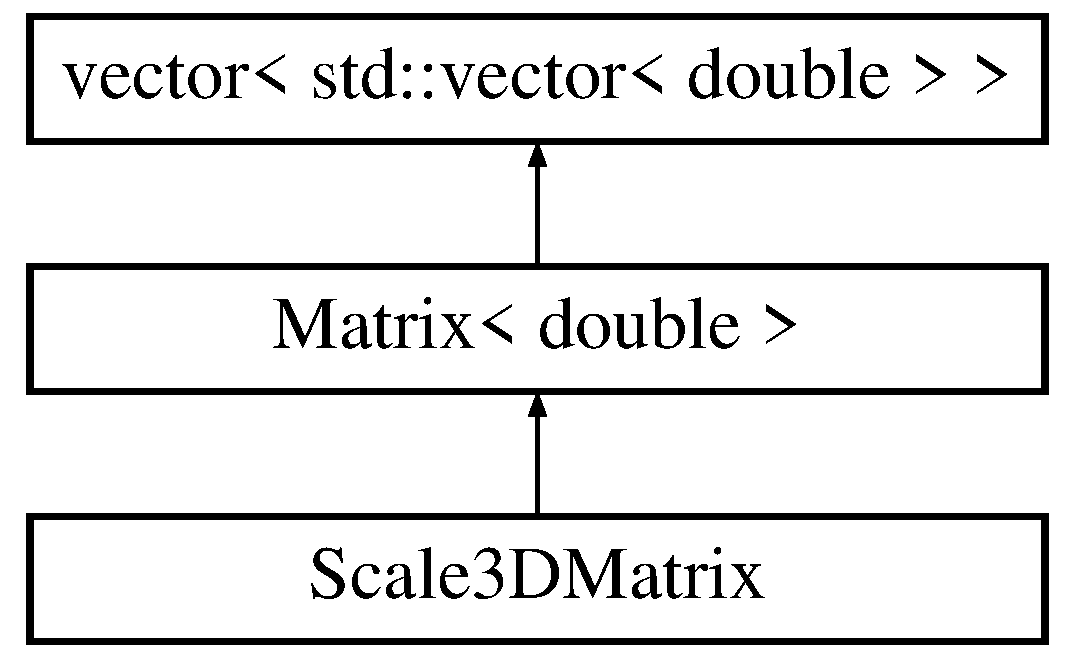
\includegraphics[height=3cm]{classScale3DMatrix}
\end{center}
\end{figure}
\subsection*{Public Methods}
\begin{CompactItemize}
\item 
{\bf Scale3DMatrix} (double x\-Scale, double y\-Scale, double z\-Scale)
\item 
{\bf Scale3DMatrix} (double scale)
\end{CompactItemize}


\subsection{Constructor \& Destructor Documentation}
\index{Scale3DMatrix@{Scale3DMatrix}!Scale3DMatrix@{Scale3DMatrix}}
\index{Scale3DMatrix@{Scale3DMatrix}!Scale3DMatrix@{Scale3DMatrix}}
\subsubsection{\setlength{\rightskip}{0pt plus 5cm}Scale3DMatrix::Scale3DMatrix (double {\em x\-Scale}, double {\em y\-Scale}, double {\em z\-Scale})\hspace{0.3cm}{\tt  [inline]}}\label{classScale3DMatrix_a0}


\index{Scale3DMatrix@{Scale3DMatrix}!Scale3DMatrix@{Scale3DMatrix}}
\index{Scale3DMatrix@{Scale3DMatrix}!Scale3DMatrix@{Scale3DMatrix}}
\subsubsection{\setlength{\rightskip}{0pt plus 5cm}Scale3DMatrix::Scale3DMatrix (double {\em scale})\hspace{0.3cm}{\tt  [inline]}}\label{classScale3DMatrix_a1}




The documentation for this class was generated from the following file:\begin{CompactItemize}
\item 
{\bf scale3dmatrix.h}\end{CompactItemize}

\section{Spline Class Reference}
\label{classSpline}\index{Spline@{Spline}}
{\tt \#include $<$spline.h$>$}

Inheritance diagram for Spline::\begin{figure}[H]
\begin{center}
\leavevmode
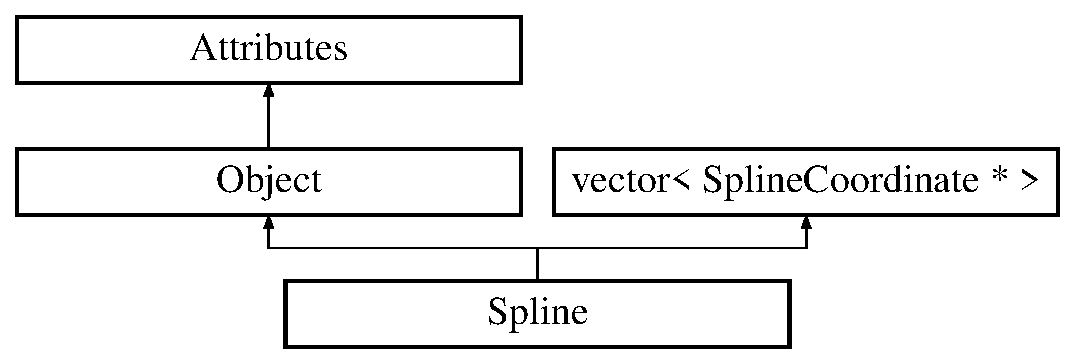
\includegraphics[height=3cm]{classSpline}
\end{center}
\end{figure}
\subsection*{Public Types}
\begin{CompactItemize}
\item 
enum {\bf Sub\-Types} \{ {\bf Opened}, 
{\bf Closed}
 \}
\end{CompactItemize}
\subsection*{Public Methods}
\begin{CompactItemize}
\item 
{\bf Spline} ()
\item 
{\bf Spline} ({\bf Spline\-Coordinate} $\ast$, {\bf Spline\-Coordinate} $\ast$)
\item 
{\bf $\sim$Spline} ()
\item 
void {\bf set\-Sub\-Type} ({\bf Sub\-Types} {\bf sub\-Type})
\item 
{\bf Sub\-Types} {\bf get\-Sub\-Type} ()
\item 
void {\bf write} (std::ostream \&stream) const
\end{CompactItemize}
\subsection*{Private Attributes}
\begin{CompactItemize}
\item 
{\bf Sub\-Types} {\bf sub\-Type}
\end{CompactItemize}


\subsection{Detailed Description}
This class handles spline objects. This class is derived from {\bf Object} {\rm (p.\,\pageref{classObject})}. \begin{Desc}
\item[Author: ]\par
Anthony Liekens \end{Desc}




\subsection{Member Enumeration Documentation}
\index{Spline@{Spline}!SubTypes@{SubTypes}}
\index{SubTypes@{SubTypes}!Spline@{Spline}}
\subsubsection{\setlength{\rightskip}{0pt plus 5cm}enum Spline::Sub\-Types}\label{classSpline_s2}


\begin{Desc}
\item[Enumeration values: ]\par
\begin{description}
\index{Opened@{Opened}!Spline@{Spline}}\index{Spline@{Spline}!Opened@{Opened}}\item[{\em 
{\em Opened}\label{classSpline_s2s0}
}]\index{Closed@{Closed}!Spline@{Spline}}\index{Spline@{Spline}!Closed@{Closed}}\item[{\em 
{\em Closed}\label{classSpline_s2s1}
}]\end{description}
\end{Desc}



\subsection{Constructor \& Destructor Documentation}
\index{Spline@{Spline}!Spline@{Spline}}
\index{Spline@{Spline}!Spline@{Spline}}
\subsubsection{\setlength{\rightskip}{0pt plus 5cm}Spline::Spline ()}\label{classSpline_a0}


\index{Spline@{Spline}!Spline@{Spline}}
\index{Spline@{Spline}!Spline@{Spline}}
\subsubsection{\setlength{\rightskip}{0pt plus 5cm}Spline::Spline ({\bf Spline\-Coordinate} $\ast$, {\bf Spline\-Coordinate} $\ast$)}\label{classSpline_a1}


\index{Spline@{Spline}!~Spline@{$\sim$Spline}}
\index{~Spline@{$\sim$Spline}!Spline@{Spline}}
\subsubsection{\setlength{\rightskip}{0pt plus 5cm}Spline::$\sim$Spline ()}\label{classSpline_a2}




\subsection{Member Function Documentation}
\index{Spline@{Spline}!getSubType@{getSubType}}
\index{getSubType@{getSubType}!Spline@{Spline}}
\subsubsection{\setlength{\rightskip}{0pt plus 5cm}{\bf Sub\-Types} Spline::get\-Sub\-Type ()\hspace{0.3cm}{\tt  [inline]}}\label{classSpline_a4}


\index{Spline@{Spline}!setSubType@{setSubType}}
\index{setSubType@{setSubType}!Spline@{Spline}}
\subsubsection{\setlength{\rightskip}{0pt plus 5cm}void Spline::set\-Sub\-Type ({\bf Sub\-Types} {\em sub\-Type})\hspace{0.3cm}{\tt  [inline]}}\label{classSpline_a3}


\index{Spline@{Spline}!write@{write}}
\index{write@{write}!Spline@{Spline}}
\subsubsection{\setlength{\rightskip}{0pt plus 5cm}void Spline::write (std::ostream \& {\em stream}) const\hspace{0.3cm}{\tt  [virtual]}}\label{classSpline_a5}


Write the object to a given outstream. All inherited classes of object should provide this method, since it's called by {\bf Figure} {\rm (p.\,\pageref{classFigure})} (the object container) to output objects to a given stream. \begin{Desc}
\item[Parameters: ]\par
\begin{description}
\item[{\em 
stream}]output stream \end{description}
\end{Desc}
\begin{Desc}
\item[Returns: ]\par
void \end{Desc}


Reimplemented from {\bf Object} {\rm (p.\,\pageref{classObject_a3})}.

\subsection{Member Data Documentation}
\index{Spline@{Spline}!subType@{subType}}
\index{subType@{subType}!Spline@{Spline}}
\subsubsection{\setlength{\rightskip}{0pt plus 5cm}{\bf Sub\-Types} Spline::sub\-Type\hspace{0.3cm}{\tt  [private]}}\label{classSpline_o0}




The documentation for this class was generated from the following files:\begin{CompactItemize}
\item 
{\bf spline.h}\item 
{\bf spline.cpp}\end{CompactItemize}

\section{Spline\-Coordinate Class Reference}
\label{classSplineCoordinate}\index{SplineCoordinate@{SplineCoordinate}}
{\tt \#include $<$splinecoordinate.h$>$}

Inheritance diagram for Spline\-Coordinate::\begin{figure}[H]
\begin{center}
\leavevmode
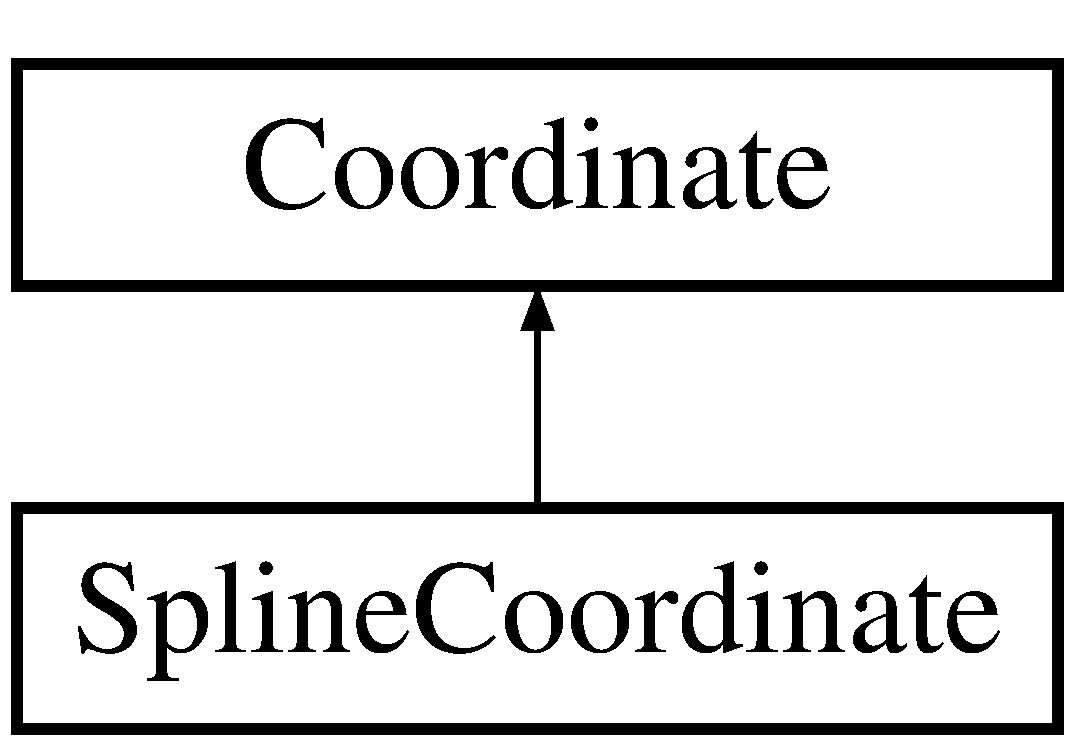
\includegraphics[height=2cm]{classSplineCoordinate}
\end{center}
\end{figure}
\subsection*{Public Methods}
\begin{CompactItemize}
\item 
{\bf Spline\-Coordinate} ()
\item 
{\bf Spline\-Coordinate} (int {\bf x}, int {\bf y}, float {\bf shape\-Factor})
\item 
{\bf Spline\-Coordinate} ({\bf Coordinate} $\ast$c, float shapefactor)
\item 
{\bf $\sim$Spline\-Coordinate} ()
\item 
void {\bf set\-Shape\-Factor} (float {\bf shape\-Factor})
\item 
float {\bf get\-Shape\-Factor} ()
\end{CompactItemize}
\subsection*{Private Attributes}
\begin{CompactItemize}
\item 
float {\bf shape\-Factor}
\end{CompactItemize}


\subsection{Detailed Description}
This class handles coordinates to be used in splines. This class is derived from {\bf Coordinate} {\rm (p.\,\pageref{classCoordinate})}. \begin{Desc}
\item[Author: ]\par
Anthony Liekens \end{Desc}




\subsection{Constructor \& Destructor Documentation}
\index{SplineCoordinate@{Spline\-Coordinate}!SplineCoordinate@{SplineCoordinate}}
\index{SplineCoordinate@{SplineCoordinate}!SplineCoordinate@{Spline\-Coordinate}}
\subsubsection{\setlength{\rightskip}{0pt plus 5cm}Spline\-Coordinate::Spline\-Coordinate ()}\label{classSplineCoordinate_a0}


Constructor. Constructs a spline coordinate. \index{SplineCoordinate@{Spline\-Coordinate}!SplineCoordinate@{SplineCoordinate}}
\index{SplineCoordinate@{SplineCoordinate}!SplineCoordinate@{Spline\-Coordinate}}
\subsubsection{\setlength{\rightskip}{0pt plus 5cm}Spline\-Coordinate::Spline\-Coordinate (int {\em x}, int {\em y}, float {\em shape\-Factor})}\label{classSplineCoordinate_a1}


Constructor. Constructs a spline coordinate. \begin{Desc}
\item[Parameters: ]\par
\begin{description}
\item[{\em 
x}]X-axis value of the coordinate \item[{\em 
y}]Y-axis value of the coordinate \item[{\em 
shape\-Factor}]The value of this factor must be between -1 (which means that the spline is interpolated at this point) and 1 (which means that the spline is approximated at this point). The spline is always smooth in the neighbourhood of a control point, except when the value of the factor is 0 for which there is a first-order discontinuity (i.e. angular point). \end{description}
\end{Desc}
\index{SplineCoordinate@{Spline\-Coordinate}!SplineCoordinate@{SplineCoordinate}}
\index{SplineCoordinate@{SplineCoordinate}!SplineCoordinate@{Spline\-Coordinate}}
\subsubsection{\setlength{\rightskip}{0pt plus 5cm}Spline\-Coordinate::Spline\-Coordinate ({\bf Coordinate} $\ast$ {\em c}, float {\em shapefactor})}\label{classSplineCoordinate_a2}


Constructor. Constructs a spline coordinate. \begin{Desc}
\item[Parameters: ]\par
\begin{description}
\item[{\em 
c}]{\bf Coordinate} {\rm (p.\,\pageref{classCoordinate})} of the spline coordinate \item[{\em 
shape\-Factor}]The value of this factor must be between -1 (which means that the spline is interpolated at this point) and 1 (which means that the spline is approximated at this point). The spline is always smooth in the neighbourhood of a control point, except when the value of the factor is 0 for which there is a first-order discontinuity (i.e. angular point). \end{description}
\end{Desc}
\index{SplineCoordinate@{Spline\-Coordinate}!~SplineCoordinate@{$\sim$SplineCoordinate}}
\index{~SplineCoordinate@{$\sim$SplineCoordinate}!SplineCoordinate@{Spline\-Coordinate}}
\subsubsection{\setlength{\rightskip}{0pt plus 5cm}Spline\-Coordinate::$\sim$Spline\-Coordinate ()}\label{classSplineCoordinate_a3}


Destructor. Destructs a spline coordinate. 

\subsection{Member Function Documentation}
\index{SplineCoordinate@{Spline\-Coordinate}!getShapeFactor@{getShapeFactor}}
\index{getShapeFactor@{getShapeFactor}!SplineCoordinate@{Spline\-Coordinate}}
\subsubsection{\setlength{\rightskip}{0pt plus 5cm}float Spline\-Coordinate::get\-Shape\-Factor ()\hspace{0.3cm}{\tt  [inline]}}\label{classSplineCoordinate_a5}


Returns the shape factor. \begin{Desc}
\item[Returns: ]\par
float \end{Desc}
\index{SplineCoordinate@{Spline\-Coordinate}!setShapeFactor@{setShapeFactor}}
\index{setShapeFactor@{setShapeFactor}!SplineCoordinate@{Spline\-Coordinate}}
\subsubsection{\setlength{\rightskip}{0pt plus 5cm}void Spline\-Coordinate::set\-Shape\-Factor (float {\em shape\-Factor})\hspace{0.3cm}{\tt  [inline]}}\label{classSplineCoordinate_a4}


Set the shape factor \begin{Desc}
\item[Parameters: ]\par
\begin{description}
\item[{\em 
shape\-Factor}]The value of this factor must be between -1 (which means that the spline is interpolated at this point) and 1 (which means that the spline is approximated at this point). The spline is always smooth in the neighbourhood of a control point, except when the value of the factor is 0 for which there is a first-order discontinuity (i.e. angular point). \end{description}
\end{Desc}
\begin{Desc}
\item[Returns: ]\par
void \end{Desc}


\subsection{Member Data Documentation}
\index{SplineCoordinate@{Spline\-Coordinate}!shapeFactor@{shapeFactor}}
\index{shapeFactor@{shapeFactor}!SplineCoordinate@{Spline\-Coordinate}}
\subsubsection{\setlength{\rightskip}{0pt plus 5cm}float Spline\-Coordinate::shape\-Factor\hspace{0.3cm}{\tt  [private]}}\label{classSplineCoordinate_o0}




The documentation for this class was generated from the following files:\begin{CompactItemize}
\item 
{\bf splinecoordinate.h}\item 
{\bf splinecoordinate.cpp}\end{CompactItemize}

\section{Text Class Reference}
\label{classText}\index{Text@{Text}}
{\tt \#include $<$text.h$>$}

Inheritance diagram for Text::\begin{figure}[H]
\begin{center}
\leavevmode
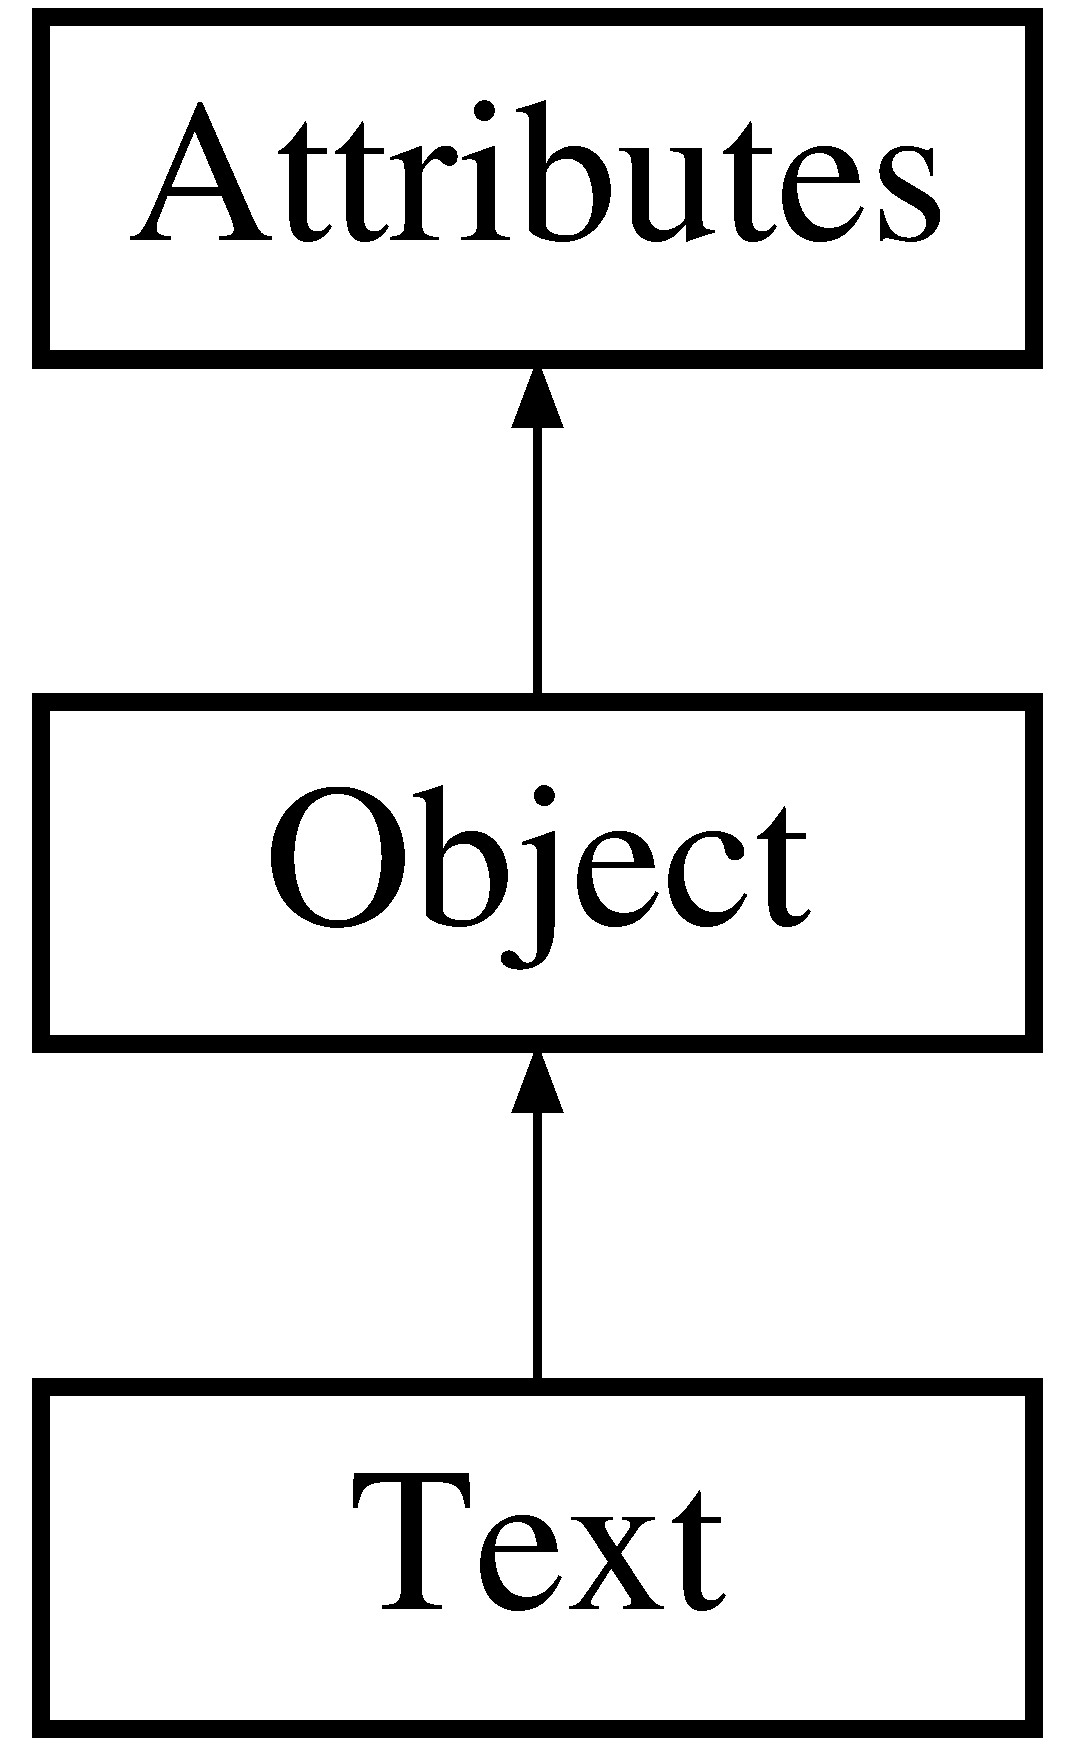
\includegraphics[height=3cm]{classText}
\end{center}
\end{figure}
\subsection*{Public Types}
\begin{CompactItemize}
\item 
enum {\bf Text\-Justifications} \{ {\bf Left\-Justified} =  0, 
{\bf Center\-Justified} =  1, 
{\bf Right\-Justified} =  2
 \}
\end{CompactItemize}
\subsection*{Public Methods}
\begin{CompactItemize}
\item 
{\bf Text} ()
\item 
{\bf Text} ({\bf Coordinate} $\ast${\bf place}, std::string {\bf contents})
\item 
{\bf $\sim$Text} ()
\item 
void {\bf set\-Justification} ({\bf Text\-Justifications} {\bf justification})
\item 
{\bf Text\-Justifications} {\bf get\-Justification} ()
\item 
void {\bf write} (std::ostream \&stream) const
\end{CompactItemize}
\subsection*{Protected Attributes}
\begin{CompactItemize}
\item 
{\bf Text\-Justifications} {\bf justification}
\item 
{\bf Coordinate} $\ast$ {\bf place}
\item 
std::string {\bf contents}
\end{CompactItemize}


\subsection{Detailed Description}
This class handles text objects. This class is derived from {\bf Object} {\rm (p.\,\pageref{classObject})}. \begin{Desc}
\item[Author: ]\par
Anthony Liekens \end{Desc}




\subsection{Member Enumeration Documentation}
\index{Text@{Text}!TextJustifications@{TextJustifications}}
\index{TextJustifications@{TextJustifications}!Text@{Text}}
\subsubsection{\setlength{\rightskip}{0pt plus 5cm}enum Text::Text\-Justifications}\label{classText_s3}


Enumeration of text justifications. The following justifications can be used to set the justification of a text object : \{$\backslash$tt Left\-Justified, Center\-Justified, Right\-Justified\} \begin{Desc}
\item[Enumeration values: ]\par
\begin{description}
\index{LeftJustified@{LeftJustified}!Text@{Text}}\index{Text@{Text}!LeftJustified@{LeftJustified}}\item[{\em 
{\em Left\-Justified}\label{classText_s3s0}
}]\index{CenterJustified@{CenterJustified}!Text@{Text}}\index{Text@{Text}!CenterJustified@{CenterJustified}}\item[{\em 
{\em Center\-Justified}\label{classText_s3s1}
}]\index{RightJustified@{RightJustified}!Text@{Text}}\index{Text@{Text}!RightJustified@{RightJustified}}\item[{\em 
{\em Right\-Justified}\label{classText_s3s2}
}]\end{description}
\end{Desc}



\subsection{Constructor \& Destructor Documentation}
\index{Text@{Text}!Text@{Text}}
\index{Text@{Text}!Text@{Text}}
\subsubsection{\setlength{\rightskip}{0pt plus 5cm}Text::Text ()}\label{classText_a0}


Constructor. Constructs a text object \index{Text@{Text}!Text@{Text}}
\index{Text@{Text}!Text@{Text}}
\subsubsection{\setlength{\rightskip}{0pt plus 5cm}Text::Text ({\bf Coordinate} $\ast$ {\em place}, std::string {\em contents})}\label{classText_a1}


Constructor. Constructs a text object \begin{Desc}
\item[Parameters: ]\par
\begin{description}
\item[{\em 
place}]- Instance of {\bf Coordinate} {\rm (p.\,\pageref{classCoordinate})}. Coordinates where the text object will be placed. \item[{\em 
contents}]- string \end{description}
\end{Desc}
\index{Text@{Text}!~Text@{$\sim$Text}}
\index{~Text@{$\sim$Text}!Text@{Text}}
\subsubsection{\setlength{\rightskip}{0pt plus 5cm}Text::$\sim$Text ()}\label{classText_a2}




\subsection{Member Function Documentation}
\index{Text@{Text}!getJustification@{getJustification}}
\index{getJustification@{getJustification}!Text@{Text}}
\subsubsection{\setlength{\rightskip}{0pt plus 5cm}{\bf Text\-Justifications} Text::get\-Justification ()\hspace{0.3cm}{\tt  [inline]}}\label{classText_a4}


Returns the text justification \begin{Desc}
\item[Returns: ]\par
Instance of {\bf Text\-Justifications} {\rm (p.\,\pageref{classText_s3})} \end{Desc}
\index{Text@{Text}!setJustification@{setJustification}}
\index{setJustification@{setJustification}!Text@{Text}}
\subsubsection{\setlength{\rightskip}{0pt plus 5cm}void Text::set\-Justification ({\bf Text\-Justifications} {\em justification})\hspace{0.3cm}{\tt  [inline]}}\label{classText_a3}


Set the text justification \begin{Desc}
\item[Parameters: ]\par
\begin{description}
\item[{\em 
justification}]{\bf Text\-Justifications} {\rm (p.\,\pageref{classText_s3})} \end{description}
\end{Desc}
\begin{Desc}
\item[Returns: ]\par
void \end{Desc}
\index{Text@{Text}!write@{write}}
\index{write@{write}!Text@{Text}}
\subsubsection{\setlength{\rightskip}{0pt plus 5cm}void Text::write (std::ostream \& {\em stream}) const\hspace{0.3cm}{\tt  [virtual]}}\label{classText_a5}


Write the text object to a given outstream. \begin{Desc}
\item[Parameters: ]\par
\begin{description}
\item[{\em 
stream}]output stream \end{description}
\end{Desc}
\begin{Desc}
\item[Returns: ]\par
void \end{Desc}


Reimplemented from {\bf Object} {\rm (p.\,\pageref{classObject_a3})}.

\subsection{Member Data Documentation}
\index{Text@{Text}!contents@{contents}}
\index{contents@{contents}!Text@{Text}}
\subsubsection{\setlength{\rightskip}{0pt plus 5cm}std::string Text::contents\hspace{0.3cm}{\tt  [protected]}}\label{classText_n2}


\index{Text@{Text}!justification@{justification}}
\index{justification@{justification}!Text@{Text}}
\subsubsection{\setlength{\rightskip}{0pt plus 5cm}{\bf Text\-Justifications} Text::justification\hspace{0.3cm}{\tt  [protected]}}\label{classText_n0}


\index{Text@{Text}!place@{place}}
\index{place@{place}!Text@{Text}}
\subsubsection{\setlength{\rightskip}{0pt plus 5cm}{\bf Coordinate}$\ast$ Text::place\hspace{0.3cm}{\tt  [protected]}}\label{classText_n1}




The documentation for this class was generated from the following files:\begin{CompactItemize}
\item 
{\bf text.h}\item 
{\bf text.cpp}\end{CompactItemize}

\section{Text3D Class Reference}
\label{classText3D}\index{Text3D@{Text3D}}
{\tt \#include $<$text3d.h$>$}

Inheritance diagram for Text3D::\begin{figure}[H]
\begin{center}
\leavevmode
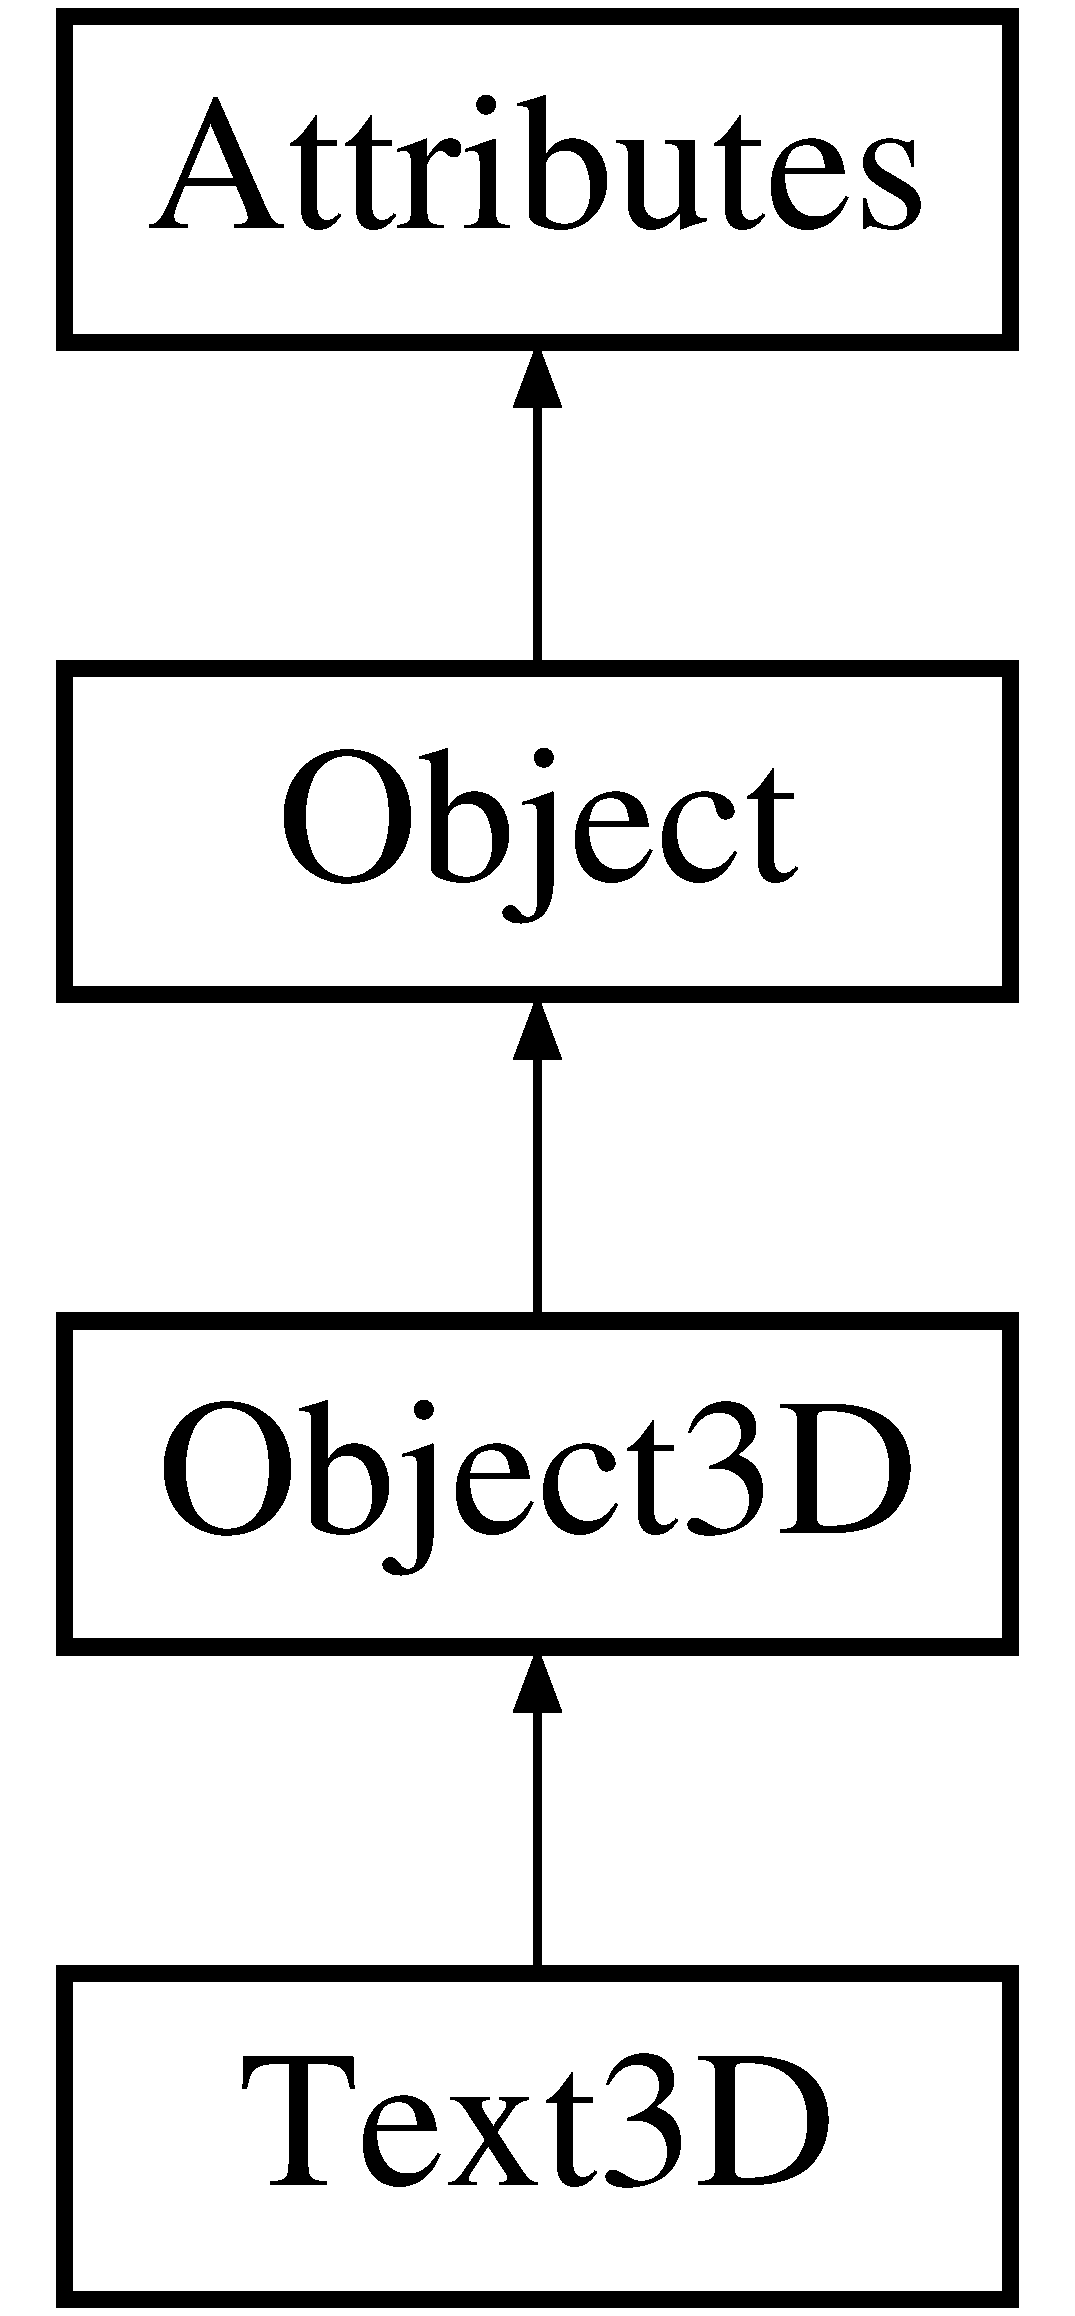
\includegraphics[height=4cm]{classText3D}
\end{center}
\end{figure}
\subsection*{Public Methods}
\begin{CompactItemize}
\item 
{\bf Text3D} ()
\item 
{\bf Text3D} ({\bf Coordinate3D} $\ast${\bf place}, std::string {\bf contents})
\item 
{\bf $\sim$Text3D} ()
\item 
void {\bf set\-Justification} ({\bf Text::Text\-Justifications} {\bf justification})
\item 
{\bf Text::Text\-Justifications} {\bf get\-Justification} ()
\item 
std::pair$<$ double, double $>$ {\bf get\-Depth\-Range} ()
\item 
void {\bf render} ({\bf Figure} $\ast$, double x\-Offset, double y\-Offset, double scale, double distance, double min\-Depth, double max\-Depth, int min\-Fig\-Depth=0, int max\-Fig\-Depth=999)
\item 
void {\bf apply\-Matrix} ({\bf Matrix}$<$ double $>$ $\ast$)
\item 
void {\bf translate} ({\bf Coordinate3D} $\ast$)
\item 
void {\bf write} (std::ostream \&stream) const
\end{CompactItemize}
\subsection*{Protected Attributes}
\begin{CompactItemize}
\item 
{\bf Text::Text\-Justifications} {\bf justification}
\item 
{\bf Coordinate3D} $\ast$ {\bf place}
\item 
std::string {\bf contents}
\end{CompactItemize}


\subsection{Detailed Description}
This class handles text objects. This class is derived from {\bf Object} {\rm (p.\,\pageref{classObject})}. \begin{Desc}
\item[Author: ]\par
Anthony Liekens \end{Desc}




\subsection{Constructor \& Destructor Documentation}
\index{Text3D@{Text3D}!Text3D@{Text3D}}
\index{Text3D@{Text3D}!Text3D@{Text3D}}
\subsubsection{\setlength{\rightskip}{0pt plus 5cm}Text3D::Text3D ()}\label{classText3D_a0}


Constructor. Constructs a text object \index{Text3D@{Text3D}!Text3D@{Text3D}}
\index{Text3D@{Text3D}!Text3D@{Text3D}}
\subsubsection{\setlength{\rightskip}{0pt plus 5cm}Text3D::Text3D ({\bf Coordinate3D} $\ast$ {\em place}, std::string {\em contents})}\label{classText3D_a1}


Constructor. Constructs a text object \begin{Desc}
\item[Parameters: ]\par
\begin{description}
\item[{\em 
place}]- Instance of {\bf Coordinate} {\rm (p.\,\pageref{classCoordinate})}. Coordinates where the text object will be placed. \item[{\em 
contents}]- string \end{description}
\end{Desc}
\index{Text3D@{Text3D}!~Text3D@{$\sim$Text3D}}
\index{~Text3D@{$\sim$Text3D}!Text3D@{Text3D}}
\subsubsection{\setlength{\rightskip}{0pt plus 5cm}Text3D::$\sim$Text3D ()}\label{classText3D_a2}




\subsection{Member Function Documentation}
\index{Text3D@{Text3D}!applyMatrix@{applyMatrix}}
\index{applyMatrix@{applyMatrix}!Text3D@{Text3D}}
\subsubsection{\setlength{\rightskip}{0pt plus 5cm}void Text3D::apply\-Matrix ({\bf Matrix}$<$ double $>$ $\ast$)\hspace{0.3cm}{\tt  [virtual]}}\label{classText3D_a7}




Implements {\bf Object3D} {\rm (p.\,\pageref{classObject3D_a2})}.\index{Text3D@{Text3D}!getDepthRange@{getDepthRange}}
\index{getDepthRange@{getDepthRange}!Text3D@{Text3D}}
\subsubsection{\setlength{\rightskip}{0pt plus 5cm}std::pair$<$ double, double $>$ Text3D::get\-Depth\-Range ()\hspace{0.3cm}{\tt  [virtual]}}\label{classText3D_a5}




Implements {\bf Object3D} {\rm (p.\,\pageref{classObject3D_a0})}.\index{Text3D@{Text3D}!getJustification@{getJustification}}
\index{getJustification@{getJustification}!Text3D@{Text3D}}
\subsubsection{\setlength{\rightskip}{0pt plus 5cm}{\bf Text::Text\-Justifications} Text3D::get\-Justification ()\hspace{0.3cm}{\tt  [inline]}}\label{classText3D_a4}


Returns the text justification \begin{Desc}
\item[Returns: ]\par
Instance of Text\-Justifications \end{Desc}
\index{Text3D@{Text3D}!render@{render}}
\index{render@{render}!Text3D@{Text3D}}
\subsubsection{\setlength{\rightskip}{0pt plus 5cm}void Text3D::render ({\bf Figure} $\ast$, double {\em x\-Offset}, double {\em y\-Offset}, double {\em scale}, double {\em distance}, double {\em min\-Depth}, double {\em max\-Depth}, int {\em min\-Fig\-Depth} = 0, int {\em max\-Fig\-Depth} = 999)\hspace{0.3cm}{\tt  [virtual]}}\label{classText3D_a6}




Implements {\bf Object3D} {\rm (p.\,\pageref{classObject3D_a1})}.\index{Text3D@{Text3D}!setJustification@{setJustification}}
\index{setJustification@{setJustification}!Text3D@{Text3D}}
\subsubsection{\setlength{\rightskip}{0pt plus 5cm}void Text3D::set\-Justification ({\bf Text::Text\-Justifications} {\em justification})\hspace{0.3cm}{\tt  [inline]}}\label{classText3D_a3}


Set the text justification \begin{Desc}
\item[Parameters: ]\par
\begin{description}
\item[{\em 
justification}]Text\-Justifications \end{description}
\end{Desc}
\begin{Desc}
\item[Returns: ]\par
void \end{Desc}
\index{Text3D@{Text3D}!translate@{translate}}
\index{translate@{translate}!Text3D@{Text3D}}
\subsubsection{\setlength{\rightskip}{0pt plus 5cm}void Text3D::translate ({\bf Coordinate3D} $\ast$)\hspace{0.3cm}{\tt  [virtual]}}\label{classText3D_a8}




Implements {\bf Object3D} {\rm (p.\,\pageref{classObject3D_a3})}.\index{Text3D@{Text3D}!write@{write}}
\index{write@{write}!Text3D@{Text3D}}
\subsubsection{\setlength{\rightskip}{0pt plus 5cm}void Text3D::write (std::ostream \& {\em stream}) const\hspace{0.3cm}{\tt  [virtual]}}\label{classText3D_a9}


Write the text object to a given outstream. \begin{Desc}
\item[Parameters: ]\par
\begin{description}
\item[{\em 
stream}]output stream \end{description}
\end{Desc}
\begin{Desc}
\item[Returns: ]\par
void \end{Desc}


Reimplemented from {\bf Object} {\rm (p.\,\pageref{classObject_a3})}.

\subsection{Member Data Documentation}
\index{Text3D@{Text3D}!contents@{contents}}
\index{contents@{contents}!Text3D@{Text3D}}
\subsubsection{\setlength{\rightskip}{0pt plus 5cm}std::string Text3D::contents\hspace{0.3cm}{\tt  [protected]}}\label{classText3D_n2}


\index{Text3D@{Text3D}!justification@{justification}}
\index{justification@{justification}!Text3D@{Text3D}}
\subsubsection{\setlength{\rightskip}{0pt plus 5cm}{\bf Text::Text\-Justifications} Text3D::justification\hspace{0.3cm}{\tt  [protected]}}\label{classText3D_n0}


\index{Text3D@{Text3D}!place@{place}}
\index{place@{place}!Text3D@{Text3D}}
\subsubsection{\setlength{\rightskip}{0pt plus 5cm}{\bf Coordinate3D}$\ast$ Text3D::place\hspace{0.3cm}{\tt  [protected]}}\label{classText3D_n1}




The documentation for this class was generated from the following files:\begin{CompactItemize}
\item 
{\bf text3d.h}\item 
{\bf text3d.cpp}\end{CompactItemize}

\section{vector Class Reference}
\label{classstd_1_1vector}\index{std::vector@{std::vector}}
Inheritance diagram for vector::\begin{figure}[H]
\begin{center}
\leavevmode
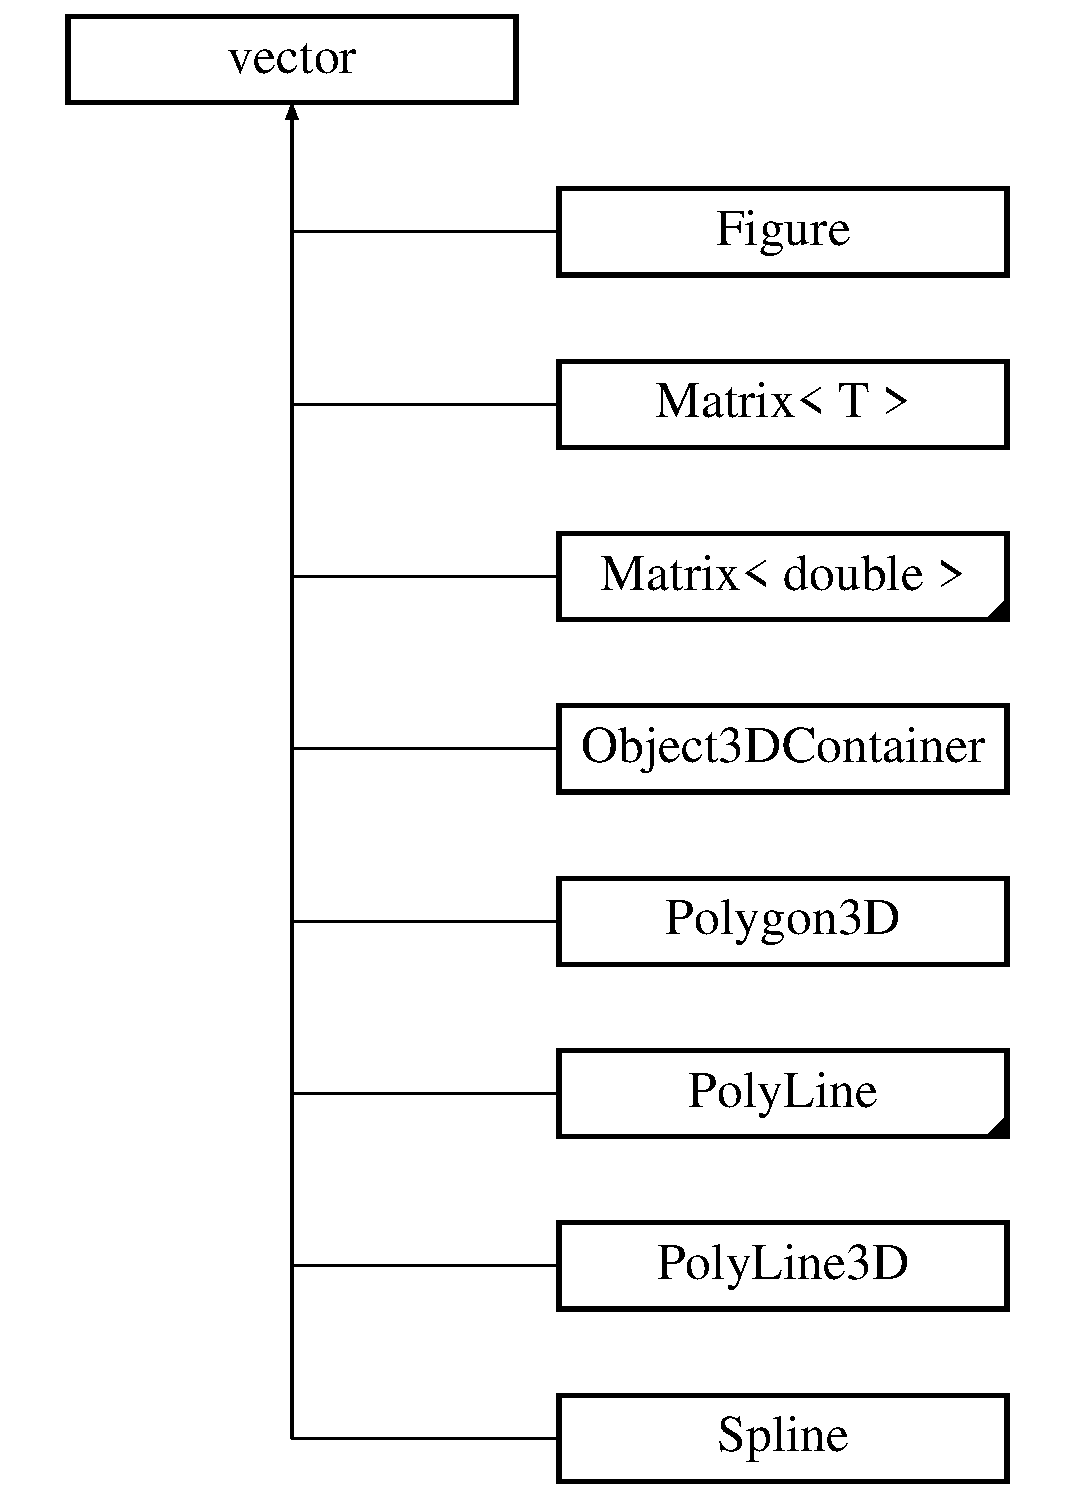
\includegraphics[height=9cm]{classstd_1_1vector}
\end{center}
\end{figure}


The documentation for this class was generated from the following file:\begin{CompactItemize}
\item 
{\bf matrix.h}\end{CompactItemize}

\chapter{Fig++ File Documentation}
\section{arc.cpp File Reference}
\label{arc_8cpp}\index{arc.cpp@{arc.cpp}}
{\tt \#include \char`\"{}arc.h\char`\"{}}\par

\section{arc.h File Reference}
\label{arc_8h}\index{arc.h@{arc.h}}
{\tt \#include \char`\"{}object.h\char`\"{}}\par
{\tt \#include \char`\"{}coordinate.h\char`\"{}}\par
\subsection*{Compounds}
\begin{CompactItemize}
\item 
class {\bf Arc}
\end{CompactItemize}
\subsection*{Functions}
\begin{CompactItemize}
\item 
std::ostream \& {\bf operator$<$$<$} (std::ostream \&stream, const {\bf Arc} \&a)
\end{CompactItemize}


\subsection{Function Documentation}
\index{arc.h@{arc.h}!operator<<@{operator$<$$<$}}
\index{operator<<@{operator$<$$<$}!arc.h@{arc.h}}
\subsubsection{\setlength{\rightskip}{0pt plus 5cm}std::ostream\& operator$<$$<$ (std::ostream \& {\em stream}, const {\bf Arc} \& {\em a})\hspace{0.3cm}{\tt  [inline]}}\label{arc_8h_a0}



\section{arrow.cpp File Reference}
\label{arrow_8cpp}\index{arrow.cpp@{arrow.cpp}}
{\tt \#include \char`\"{}arrow.h\char`\"{}}\par

\section{arrow.h File Reference}
\label{arrow_8h}\index{arrow.h@{arrow.h}}
{\tt \#include $<$iostream$>$}\par
\subsection*{Compounds}
\begin{CompactItemize}
\item 
class {\bf Arrow}
\end{CompactItemize}
\subsection*{Functions}
\begin{CompactItemize}
\item 
std::ostream \& {\bf operator$<$$<$} (std::ostream \&stream, const {\bf Arrow} \&a)
\end{CompactItemize}


\subsection{Function Documentation}
\index{arrow.h@{arrow.h}!operator<<@{operator$<$$<$}}
\index{operator<<@{operator$<$$<$}!arrow.h@{arrow.h}}
\subsubsection{\setlength{\rightskip}{0pt plus 5cm}std::ostream\& operator$<$$<$ (std::ostream \& {\em stream}, const {\bf Arrow} \& {\em a})\hspace{0.3cm}{\tt  [inline]}}\label{arrow_8h_a0}



\section{attributes.cpp File Reference}
\label{attributes_8cpp}\index{attributes.cpp@{attributes.cpp}}
{\tt \#include \char`\"{}attributes.h\char`\"{}}\par

\section{attributes.h File Reference}
\label{attributes_8h}\index{attributes.h@{attributes.h}}
{\tt \#include \char`\"{}arrow.h\char`\"{}}\par
\subsection*{Compounds}
\begin{CompactItemize}
\item 
class {\bf Attributes}
\end{CompactItemize}

\section{box.cpp File Reference}
\label{box_8cpp}\index{box.cpp@{box.cpp}}
{\tt \#include \char`\"{}box.h\char`\"{}}\par

\section{box.h File Reference}
\label{box_8h}\index{box.h@{box.h}}
{\tt \#include \char`\"{}polyline.h\char`\"{}}\par
\subsection*{Compounds}
\begin{CompactItemize}
\item 
class {\bf Box}
\end{CompactItemize}

\section{coordinate.cpp File Reference}
\label{coordinate_8cpp}\index{coordinate.cpp@{coordinate.cpp}}
{\tt \#include \char`\"{}coordinate.h\char`\"{}}\par

\section{coordinate.h File Reference}
\label{coordinate_8h}\index{coordinate.h@{coordinate.h}}
{\tt \#include $<$math.h$>$}\par
{\tt \#include $<$iostream$>$}\par
\subsection*{Compounds}
\begin{CompactItemize}
\item 
class {\bf Coordinate}
\end{CompactItemize}
\subsection*{Functions}
\begin{CompactItemize}
\item 
std::ostream \& {\bf operator$<$$<$} (std::ostream \&stream, const {\bf Coordinate} \&c)
\end{CompactItemize}


\subsection{Function Documentation}
\index{coordinate.h@{coordinate.h}!operator<<@{operator$<$$<$}}
\index{operator<<@{operator$<$$<$}!coordinate.h@{coordinate.h}}
\subsubsection{\setlength{\rightskip}{0pt plus 5cm}std::ostream\& operator$<$$<$ (std::ostream \& {\em stream}, const {\bf Coordinate} \& {\em c})\hspace{0.3cm}{\tt  [inline]}}\label{coordinate_8h_a0}



\section{coordinate3d.cpp File Reference}
\label{coordinate3d_8cpp}\index{coordinate3d.cpp@{coordinate3d.cpp}}
{\tt \#include \char`\"{}coordinate3d.h\char`\"{}}\par

\section{coordinate3d.h File Reference}
\label{coordinate3d_8h}\index{coordinate3d.h@{coordinate3d.h}}
{\tt \#include $<$math.h$>$}\par
{\tt \#include $<$iostream$>$}\par
{\tt \#include \char`\"{}coordinate.h\char`\"{}}\par
{\tt \#include \char`\"{}matrix.h\char`\"{}}\par
\subsection*{Compounds}
\begin{CompactItemize}
\item 
class {\bf Coordinate3D}
\end{CompactItemize}
\subsection*{Functions}
\begin{CompactItemize}
\item 
std::ostream \& {\bf operator$<$$<$} (std::ostream \&stream, const {\bf Coordinate3D} \&c)
\end{CompactItemize}


\subsection{Function Documentation}
\index{coordinate3d.h@{coordinate3d.h}!operator<<@{operator$<$$<$}}
\index{operator<<@{operator$<$$<$}!coordinate3d.h@{coordinate3d.h}}
\subsubsection{\setlength{\rightskip}{0pt plus 5cm}std::ostream\& operator$<$$<$ (std::ostream \& {\em stream}, const {\bf Coordinate3D} \& {\em c})\hspace{0.3cm}{\tt  [inline]}}\label{coordinate3d_8h_a0}



\section{diametercircle.cpp File Reference}
\label{diametercircle_8cpp}\index{diametercircle.cpp@{diametercircle.cpp}}
{\tt \#include \char`\"{}diametercircle.h\char`\"{}}\par

\section{diametercircle.h File Reference}
\label{diametercircle_8h}\index{diametercircle.h@{diametercircle.h}}
{\tt \#include \char`\"{}ellipse.h\char`\"{}}\par
\subsection*{Compounds}
\begin{CompactItemize}
\item 
class {\bf Diameter\-Circle}
\end{CompactItemize}

\section{diameterellipse.cpp File Reference}
\label{diameterellipse_8cpp}\index{diameterellipse.cpp@{diameterellipse.cpp}}
{\tt \#include \char`\"{}diameterellipse.h\char`\"{}}\par

\section{diameterellipse.h File Reference}
\label{diameterellipse_8h}\index{diameterellipse.h@{diameterellipse.h}}
{\tt \#include $<$math.h$>$}\par
{\tt \#include \char`\"{}ellipse.h\char`\"{}}\par
\subsection*{Compounds}
\begin{CompactItemize}
\item 
class {\bf Diameter\-Ellipse}
\end{CompactItemize}

\section{ellipse.cpp File Reference}
\label{ellipse_8cpp}\index{ellipse.cpp@{ellipse.cpp}}
{\tt \#include \char`\"{}ellipse.h\char`\"{}}\par

\section{ellipse.h File Reference}
\label{ellipse_8h}\index{ellipse.h@{ellipse.h}}
{\tt \#include \char`\"{}object.h\char`\"{}}\par
{\tt \#include \char`\"{}coordinate.h\char`\"{}}\par
\subsection*{Compounds}
\begin{CompactItemize}
\item 
class {\bf Ellipse}
\end{CompactItemize}
\subsection*{Functions}
\begin{CompactItemize}
\item 
std::ostream \& {\bf operator$<$$<$} (std::ostream \&stream, const {\bf Ellipse} \&o)
\end{CompactItemize}


\subsection{Function Documentation}
\index{ellipse.h@{ellipse.h}!operator<<@{operator$<$$<$}}
\index{operator<<@{operator$<$$<$}!ellipse.h@{ellipse.h}}
\subsubsection{\setlength{\rightskip}{0pt plus 5cm}std::ostream\& operator$<$$<$ (std::ostream \& {\em stream}, const {\bf Ellipse} \& {\em o})\hspace{0.3cm}{\tt  [inline]}}\label{ellipse_8h_a0}



\section{fig.h File Reference}
\label{fig_8h}\index{fig.h@{fig.h}}
{\tt \#include \char`\"{}arc.h\char`\"{}}\par
{\tt \#include \char`\"{}attributes.h\char`\"{}}\par
{\tt \#include \char`\"{}coordinate.h\char`\"{}}\par
{\tt \#include \char`\"{}diameterellipse.h\char`\"{}}\par
{\tt \#include \char`\"{}figure.h\char`\"{}}\par
{\tt \#include \char`\"{}polygon.h\char`\"{}}\par
{\tt \#include \char`\"{}radiiellipse.h\char`\"{}}\par
{\tt \#include \char`\"{}splinecoordinate.h\char`\"{}}\par
{\tt \#include \char`\"{}text.h\char`\"{}}\par
{\tt \#include \char`\"{}arrow.h\char`\"{}}\par
{\tt \#include \char`\"{}box.h\char`\"{}}\par
{\tt \#include \char`\"{}diametercircle.h\char`\"{}}\par
{\tt \#include \char`\"{}ellipse.h\char`\"{}}\par
{\tt \#include \char`\"{}object.h\char`\"{}}\par
{\tt \#include \char`\"{}polyline.h\char`\"{}}\par
{\tt \#include \char`\"{}radiuscircle.h\char`\"{}}\par
{\tt \#include \char`\"{}spline.h\char`\"{}}\par
{\tt \#include \char`\"{}coordinate3d.h\char`\"{}}\par
{\tt \#include \char`\"{}object3dcontainer.h\char`\"{}}\par
{\tt \#include \char`\"{}object3d.h\char`\"{}}\par
{\tt \#include \char`\"{}polygon3d.h\char`\"{}}\par
{\tt \#include \char`\"{}polyline3d.h\char`\"{}}\par
{\tt \#include \char`\"{}rotation3dmatrix.h\char`\"{}}\par
{\tt \#include \char`\"{}scale3dmatrix.h\char`\"{}}\par
{\tt \#include \char`\"{}text3d.h\char`\"{}}\par

\section{figure.cpp File Reference}
\label{figure_8cpp}\index{figure.cpp@{figure.cpp}}
{\tt \#include \char`\"{}figure.h\char`\"{}}\par

\section{figure.h File Reference}
\label{figure_8h}\index{figure.h@{figure.h}}
{\tt \#include \char`\"{}object.h\char`\"{}}\par
{\tt \#include $<$vector$>$}\par
{\tt \#include $<$iostream$>$}\par
\subsection*{Compounds}
\begin{CompactItemize}
\item 
class {\bf Figure}
\end{CompactItemize}
\subsection*{Functions}
\begin{CompactItemize}
\item 
std::ostream \& {\bf operator$<$$<$} (std::ostream \&stream, const {\bf Figure} \&f)
\end{CompactItemize}


\subsection{Function Documentation}
\index{figure.h@{figure.h}!operator<<@{operator$<$$<$}}
\index{operator<<@{operator$<$$<$}!figure.h@{figure.h}}
\subsubsection{\setlength{\rightskip}{0pt plus 5cm}std::ostream\& operator$<$$<$ (std::ostream \& {\em stream}, const {\bf Figure} \& {\em f})\hspace{0.3cm}{\tt  [inline]}}\label{figure_8h_a0}



\section{matrix.cpp File Reference}
\label{matrix_8cpp}\index{matrix.cpp@{matrix.cpp}}
{\tt \#include \char`\"{}matrix.h\char`\"{}}\par

\section{matrix.h File Reference}
\label{matrix_8h}\index{matrix.h@{matrix.h}}
{\tt \#include $<$vector$>$}\par
\subsection*{Compounds}
\begin{CompactItemize}
\item 
class {\bf Matrix}
\end{CompactItemize}

\section{object.cpp File Reference}
\label{object_8cpp}\index{object.cpp@{object.cpp}}
{\tt \#include \char`\"{}object.h\char`\"{}}\par

\section{object.h File Reference}
\label{object_8h}\index{object.h@{object.h}}
{\tt \#include $<$iostream$>$}\par
{\tt \#include \char`\"{}attributes.h\char`\"{}}\par
\subsection*{Compounds}
\begin{CompactItemize}
\item 
class {\bf Object}
\end{CompactItemize}
\subsection*{Functions}
\begin{CompactItemize}
\item 
std::ostream \& {\bf operator$<$$<$} (std::ostream \&stream, const {\bf Object} \&o)
\end{CompactItemize}


\subsection{Function Documentation}
\index{object.h@{object.h}!operator<<@{operator$<$$<$}}
\index{operator<<@{operator$<$$<$}!object.h@{object.h}}
\subsubsection{\setlength{\rightskip}{0pt plus 5cm}std::ostream\& operator$<$$<$ (std::ostream \& {\em stream}, const {\bf Object} \& {\em o})\hspace{0.3cm}{\tt  [inline]}}\label{object_8h_a0}



\section{object3d.cpp File Reference}
\label{object3d_8cpp}\index{object3d.cpp@{object3d.cpp}}
{\tt \#include \char`\"{}object3d.h\char`\"{}}\par

\section{object3d.h File Reference}
\label{object3d_8h}\index{object3d.h@{object3d.h}}
{\tt \#include \char`\"{}object.h\char`\"{}}\par
{\tt \#include \char`\"{}figure.h\char`\"{}}\par
{\tt \#include \char`\"{}matrix.h\char`\"{}}\par
{\tt \#include \char`\"{}coordinate3d.h\char`\"{}}\par
{\tt \#include $<$map$>$}\par
\subsection*{Compounds}
\begin{CompactItemize}
\item 
class {\bf Object3D}
\end{CompactItemize}

\section{object3dcontainer.cpp File Reference}
\label{object3dcontainer_8cpp}\index{object3dcontainer.cpp@{object3dcontainer.cpp}}
{\tt \#include \char`\"{}object3dcontainer.h\char`\"{}}\par
{\tt \#include $<$map$>$}\par

\section{object3dcontainer.h File Reference}
\label{object3dcontainer_8h}\index{object3dcontainer.h@{object3dcontainer.h}}
{\tt \#include \char`\"{}object3d.h\char`\"{}}\par
{\tt \#include \char`\"{}coordinate3d.h\char`\"{}}\par
{\tt \#include \char`\"{}figure.h\char`\"{}}\par
{\tt \#include \char`\"{}matrix.h\char`\"{}}\par
{\tt \#include $<$vector$>$}\par
\subsection*{Compounds}
\begin{CompactItemize}
\item 
class {\bf Object3DContainer}
\end{CompactItemize}

\section{polygon.cpp File Reference}
\label{polygon_8cpp}\index{polygon.cpp@{polygon.cpp}}
{\tt \#include \char`\"{}polygon.h\char`\"{}}\par

\section{polygon.h File Reference}
\label{polygon_8h}\index{polygon.h@{polygon.h}}
{\tt \#include \char`\"{}polyline.h\char`\"{}}\par
\subsection*{Compounds}
\begin{CompactItemize}
\item 
class {\bf Polygon}
\end{CompactItemize}

\section{polygon3d.cpp File Reference}
\label{polygon3d_8cpp}\index{polygon3d.cpp@{polygon3d.cpp}}
{\tt \#include \char`\"{}polygon3d.h\char`\"{}}\par
{\tt \#include \char`\"{}polygon.h\char`\"{}}\par

\section{polygon3d.h File Reference}
\label{polygon3d_8h}\index{polygon3d.h@{polygon3d.h}}
{\tt \#include $<$vector$>$}\par
{\tt \#include \char`\"{}polygon.h\char`\"{}}\par
{\tt \#include \char`\"{}object3d.h\char`\"{}}\par
{\tt \#include \char`\"{}coordinate3d.h\char`\"{}}\par
{\tt \#include $<$map$>$}\par
\subsection*{Compounds}
\begin{CompactItemize}
\item 
class {\bf Polygon3D}
\end{CompactItemize}
\subsection*{Functions}
\begin{CompactItemize}
\item 
std::ostream \& {\bf operator$<$$<$} (std::ostream \&stream, const {\bf Polygon3D} \&p)
\end{CompactItemize}


\subsection{Function Documentation}
\index{polygon3d.h@{polygon3d.h}!operator<<@{operator$<$$<$}}
\index{operator<<@{operator$<$$<$}!polygon3d.h@{polygon3d.h}}
\subsubsection{\setlength{\rightskip}{0pt plus 5cm}std::ostream\& operator$<$$<$ (std::ostream \& {\em stream}, const {\bf Polygon3D} \& {\em p})\hspace{0.3cm}{\tt  [inline]}}\label{polygon3d_8h_a0}



\section{polyline.cpp File Reference}
\label{polyline_8cpp}\index{polyline.cpp@{polyline.cpp}}
{\tt \#include \char`\"{}polyline.h\char`\"{}}\par

\section{polyline.h File Reference}
\label{polyline_8h}\index{polyline.h@{polyline.h}}
{\tt \#include $<$vector$>$}\par
{\tt \#include $<$iostream$>$}\par
{\tt \#include \char`\"{}object.h\char`\"{}}\par
{\tt \#include \char`\"{}coordinate.h\char`\"{}}\par
\subsection*{Compounds}
\begin{CompactItemize}
\item 
class {\bf Poly\-Line}
\end{CompactItemize}
\subsection*{Functions}
\begin{CompactItemize}
\item 
std::ostream \& {\bf operator$<$$<$} (std::ostream \&stream, const {\bf Poly\-Line} \&p)
\end{CompactItemize}


\subsection{Function Documentation}
\index{polyline.h@{polyline.h}!operator<<@{operator$<$$<$}}
\index{operator<<@{operator$<$$<$}!polyline.h@{polyline.h}}
\subsubsection{\setlength{\rightskip}{0pt plus 5cm}std::ostream\& operator$<$$<$ (std::ostream \& {\em stream}, const {\bf Poly\-Line} \& {\em p})\hspace{0.3cm}{\tt  [inline]}}\label{polyline_8h_a0}



\section{polyline3d.cpp File Reference}
\label{polyline3d_8cpp}\index{polyline3d.cpp@{polyline3d.cpp}}
{\tt \#include \char`\"{}polyline3d.h\char`\"{}}\par
{\tt \#include \char`\"{}polyline.h\char`\"{}}\par

\section{polyline3d.h File Reference}
\label{polyline3d_8h}\index{polyline3d.h@{polyline3d.h}}
{\tt \#include $<$vector$>$}\par
{\tt \#include \char`\"{}polyline.h\char`\"{}}\par
{\tt \#include \char`\"{}object3d.h\char`\"{}}\par
{\tt \#include \char`\"{}coordinate3d.h\char`\"{}}\par
{\tt \#include $<$map$>$}\par
\subsection*{Compounds}
\begin{CompactItemize}
\item 
class {\bf Poly\-Line3D}
\end{CompactItemize}
\subsection*{Functions}
\begin{CompactItemize}
\item 
std::ostream \& {\bf operator$<$$<$} (std::ostream \&stream, const {\bf Poly\-Line3D} \&p)
\end{CompactItemize}


\subsection{Function Documentation}
\index{polyline3d.h@{polyline3d.h}!operator<<@{operator$<$$<$}}
\index{operator<<@{operator$<$$<$}!polyline3d.h@{polyline3d.h}}
\subsubsection{\setlength{\rightskip}{0pt plus 5cm}std::ostream\& operator$<$$<$ (std::ostream \& {\em stream}, const {\bf Poly\-Line3D} \& {\em p})\hspace{0.3cm}{\tt  [inline]}}\label{polyline3d_8h_a0}



\section{radiiellipse.cpp File Reference}
\label{radiiellipse_8cpp}\index{radiiellipse.cpp@{radiiellipse.cpp}}
{\tt \#include \char`\"{}radiiellipse.h\char`\"{}}\par

\section{radiiellipse.h File Reference}
\label{radiiellipse_8h}\index{radiiellipse.h@{radiiellipse.h}}
{\tt \#include \char`\"{}ellipse.h\char`\"{}}\par
\subsection*{Compounds}
\begin{CompactItemize}
\item 
class {\bf Radii\-Ellipse}
\end{CompactItemize}

\section{radiuscircle.cpp File Reference}
\label{radiuscircle_8cpp}\index{radiuscircle.cpp@{radiuscircle.cpp}}
{\tt \#include \char`\"{}radiuscircle.h\char`\"{}}\par

\section{radiuscircle.h File Reference}
\label{radiuscircle_8h}\index{radiuscircle.h@{radiuscircle.h}}
{\tt \#include \char`\"{}ellipse.h\char`\"{}}\par
\subsection*{Compounds}
\begin{CompactItemize}
\item 
class {\bf Radius\-Circle}
\end{CompactItemize}

\section{rotation3dmatrix.cpp File Reference}
\label{rotation3dmatrix_8cpp}\index{rotation3dmatrix.cpp@{rotation3dmatrix.cpp}}
{\tt \#include \char`\"{}rotation3dmatrix.h\char`\"{}}\par

\section{rotation3dmatrix.h File Reference}
\label{rotation3dmatrix_8h}\index{rotation3dmatrix.h@{rotation3dmatrix.h}}
{\tt \#include \char`\"{}matrix.h\char`\"{}}\par
{\tt \#include $<$math.h$>$}\par
\subsection*{Compounds}
\begin{CompactItemize}
\item 
class {\bf Rotation3DMatrix}
\end{CompactItemize}

\section{scale3dmatrix.cpp File Reference}
\label{scale3dmatrix_8cpp}\index{scale3dmatrix.cpp@{scale3dmatrix.cpp}}
{\tt \#include \char`\"{}scale3dmatrix.h\char`\"{}}\par

\section{scale3dmatrix.h File Reference}
\label{scale3dmatrix_8h}\index{scale3dmatrix.h@{scale3dmatrix.h}}
{\tt \#include \char`\"{}matrix.h\char`\"{}}\par
{\tt \#include $<$math.h$>$}\par
\subsection*{Compounds}
\begin{CompactItemize}
\item 
class {\bf Scale3DMatrix}
\end{CompactItemize}

\section{spline.cpp File Reference}
\label{spline_8cpp}\index{spline.cpp@{spline.cpp}}
{\tt \#include \char`\"{}spline.h\char`\"{}}\par

\section{spline.h File Reference}
\label{spline_8h}\index{spline.h@{spline.h}}
{\tt \#include $<$vector$>$}\par
{\tt \#include \char`\"{}object.h\char`\"{}}\par
{\tt \#include \char`\"{}splinecoordinate.h\char`\"{}}\par
\subsection*{Compounds}
\begin{CompactItemize}
\item 
class {\bf Spline}
\end{CompactItemize}
\subsection*{Functions}
\begin{CompactItemize}
\item 
std::ostream \& {\bf operator$<$$<$} (std::ostream \&stream, const {\bf Spline} \&s)
\end{CompactItemize}


\subsection{Function Documentation}
\index{spline.h@{spline.h}!operator<<@{operator$<$$<$}}
\index{operator<<@{operator$<$$<$}!spline.h@{spline.h}}
\subsubsection{\setlength{\rightskip}{0pt plus 5cm}std::ostream\& operator$<$$<$ (std::ostream \& {\em stream}, const {\bf Spline} \& {\em s})\hspace{0.3cm}{\tt  [inline]}}\label{spline_8h_a0}



\section{splinecoordinate.cpp File Reference}
\label{splinecoordinate_8cpp}\index{splinecoordinate.cpp@{splinecoordinate.cpp}}
{\tt \#include \char`\"{}splinecoordinate.h\char`\"{}}\par

\section{splinecoordinate.h File Reference}
\label{splinecoordinate_8h}\index{splinecoordinate.h@{splinecoordinate.h}}
{\tt \#include \char`\"{}coordinate.h\char`\"{}}\par
\subsection*{Compounds}
\begin{CompactItemize}
\item 
class {\bf Spline\-Coordinate}
\end{CompactItemize}

\section{text.cpp File Reference}
\label{text_8cpp}\index{text.cpp@{text.cpp}}
{\tt \#include \char`\"{}text.h\char`\"{}}\par

\section{text.h File Reference}
\label{text_8h}\index{text.h@{text.h}}
{\tt \#include $<$string$>$}\par
{\tt \#include \char`\"{}object.h\char`\"{}}\par
{\tt \#include \char`\"{}coordinate.h\char`\"{}}\par
\subsection*{Compounds}
\begin{CompactItemize}
\item 
class {\bf Text}
\end{CompactItemize}
\subsection*{Functions}
\begin{CompactItemize}
\item 
std::ostream \& {\bf operator$<$$<$} (std::ostream \&stream, const {\bf Text} \&o)
\end{CompactItemize}


\subsection{Function Documentation}
\index{text.h@{text.h}!operator<<@{operator$<$$<$}}
\index{operator<<@{operator$<$$<$}!text.h@{text.h}}
\subsubsection{\setlength{\rightskip}{0pt plus 5cm}std::ostream\& operator$<$$<$ (std::ostream \& {\em stream}, const {\bf Text} \& {\em o})\hspace{0.3cm}{\tt  [inline]}}\label{text_8h_a0}



\section{text3d.cpp File Reference}
\label{text3d_8cpp}\index{text3d.cpp@{text3d.cpp}}
{\tt \#include \char`\"{}text3d.h\char`\"{}}\par

\section{text3d.h File Reference}
\label{text3d_8h}\index{text3d.h@{text3d.h}}
{\tt \#include $<$string$>$}\par
{\tt \#include \char`\"{}text.h\char`\"{}}\par
{\tt \#include \char`\"{}object3d.h\char`\"{}}\par
{\tt \#include \char`\"{}coordinate3d.h\char`\"{}}\par
\subsection*{Compounds}
\begin{CompactItemize}
\item 
class {\bf Text3D}
\end{CompactItemize}
\subsection*{Functions}
\begin{CompactItemize}
\item 
std::ostream \& {\bf operator$<$$<$} (std::ostream \&stream, const {\bf Text3D} \&o)
\end{CompactItemize}


\subsection{Function Documentation}
\index{text3d.h@{text3d.h}!operator<<@{operator$<$$<$}}
\index{operator<<@{operator$<$$<$}!text3d.h@{text3d.h}}
\subsubsection{\setlength{\rightskip}{0pt plus 5cm}std::ostream\& operator$<$$<$ (std::ostream \& {\em stream}, const {\bf Text3D} \& {\em o})\hspace{0.3cm}{\tt  [inline]}}\label{text3d_8h_a0}



\printindex
\end{document}
